% !TeX program = lualatex
% !TeX encoding = utf8
% !TeX spellcheck = english
% !TeX version = 2020
%
% **************************************************
% Document Class Definition
% **************************************************
\documentclass[%
    paper=A4,               % paper size --> A4 is default in Germany
    twoside=false,          % onesite or twoside printing TODO: true
    openright,              % doublepage cleaning ends up right side
    parskip=half,           % spacing value / method for paragraphs
    chapterprefix=true,     % prefix for chapter marks
    11pt,                   % font size
    headings=normal,        % size of headings
    bibliography=totoc,     % include bib in toc
    listof=totoc,           % include listof entries in toc
    titlepage=on,           % own page for each title page
    captions=tableabove,    % display table captions above the float env
    chapterprefix=false,    % do not display a prefix for chapters
    appendixprefix=false,   % but display a prefix for appendix chapter
    draft=false,            % value for draft version
]{scrreprt}%
%
%
% **************************************************
% Setup YOUR thesis document in this file !
% **************************************************
% !TEX root = thesis.tex
%
\usepackage{iftex}
% **************************************************
% Files' Character Encoding
% **************************************************
\ifPDFTeX
    \usepackage[utf8]{inputenc}
\fi
%
% **************************************************
% Information and Commands for Reuse
% **************************************************
\newcommand{\thesisTitle}{Nerve Fiber Modelling and 3D-PLI Simulations:\\ A Fiber Architect Simulation Toolbox} %Modelling of 3D Nerve Fibers and their Applications in 3D-PLI
\newcommand{\thesisName}{Felix Matuschke}
\newcommand{\thesisSubject}{Documentation}
\newcommand{\thesisDate}{\today}
\newcommand{\thesisVersion}{My First Draft}
%
\newcommand{\thesisFirstReviewer}{Prof. Dr. Gunnar Schr\"{o}der}
\newcommand{\thesisFirstReviewerUniversity}{\protect{IBI-7}}
\newcommand{\thesisFirstReviewerDepartment}{Forschungszentrum J\"{u}lich}
%
\newcommand{\thesisSecondReviewer}{Prof. Dr. Katrin Amunts}
\newcommand{\thesisSecondReviewerUniversity}{\protect{INM-1}}
\newcommand{\thesisSecondReviewerDepartment}{Forschungszentrum J\"{u}lich}
%
\newcommand{\thesisFirstSupervisor}{Prof. Dr. Markus Axer}
\newcommand{\thesisFirstSupervisorUniversity}{\protect{INM-1}}
\newcommand{\thesisFirstSupervisorDepartment}{Forschungszentrum J\"{u}lich}
%
\newcommand{\thesisUniversity}{\protect{Heinrich-Heine-Universit\"{a}t D\"{u}sseldorf}}
\newcommand{\thesisUniversityDepartment}{Math.-Nat. Fakult\"{a}t}
\newcommand{\thesisUniversityInstitute}{}
\newcommand{\thesisUniversityGroup}{}
\newcommand{\thesisUniversityCity}{D\"{u}sseldorf}
\newcommand{\thesisUniversityStreetAddress}{Universitt\"{a}sstra{\ss}e 1}
\newcommand{\thesisUniversityPostalCode}{40225 D\"{u}sseldorf}
% 
\newcommand{\thesisInstitute}{\protect{Forschungszentrum J\"{u}lich}}
\newcommand{\thesisInstituteDepartment}{Institut für Neurowissenschaften und Medizin}
\newcommand{\thesisInstituteInstitute}{Strukturelle und funktionelle Organisation des Gehirns (INM-1)}
\newcommand{\thesisInstituteGroup}{Faserbahnarchitektur}
\newcommand{\thesisInstituteCity}{J\"{u}lich}
\newcommand{\thesisInstituteStreetAddress}{Wilhelm-Johnen-Stra{\ss}e}
\newcommand{\thesisInstitutePostalCode}{52428 J\"{u}lich}
%
% **************************************************
% Debug LaTeX Information
% **************************************************
\usepackage{silence}
% \WarningFilter[references]{latex} {There were undefined references}
\WarningFilter[references]{latex} {Reference }
% \listfiles
% 
% **************************************************
% User Commands
% **************************************************
% 
% \makeatletter
% \renewcommand\listoftables{%
%         \@starttoc{lot}%
% }
% \makeatother
% % 
% \makeatletter
% \renewcommand\listoffigures{%
%         \@starttoc{lof}%
% }
% \makeatother
% % 
% \makeatletter
% \renewcommand\lstlistoflistings{%
%         \@starttoc{lof}%
% }
% \makeatother
%
%
% **************************************************
% Pre cleanthesis imports
% **************************************************
\RequirePackage[dvipsnames]{xcolor}
\usepackage{tikz}
% 
% **************************************************
% Load and Configure Packages
% **************************************************
\usepackage[english]{babel} % babel system, adjust the language of the content
\PassOptionsToPackage{% setup clean thesis style
    figuresep=colon,%
    hangfigurecaption=false,%
    hangsection=true,%
    hangsubsection=true,%
    sansserif=true,%
    configurelistings=true,%
    colorize=full,%
    colortheme=bluemagenta,%
    configurebiblatex=true,%
    bibsys=biber,%
    bibfile=bib-refs,%
    bibstyle=alphabetic,%
    bibsorting=nty,%
}{cleanthesis}
\usepackage{cleanthesis}
%
% \colorlet{citeColor}{green!50!black}
% \colorlet{linkColor}{green!75!black>wheel,1,2}
% \colorlet{urlColor}{green!75!black>twheel,1,2}
\colorlet{citeColor}{violet>twheel,2,3}
\colorlet{linkColor}{violet}
\colorlet{urlColor}{violet>twheel,1,3}
% 
\hypersetup{% setup the hyperref-package options
    pdftitle={\thesisTitle},    %   - title (PDF meta)
    pdfsubject={\thesisSubject},%   - subject (PDF meta)
    pdfauthor={\thesisName},    %   - author (PDF meta)
    plainpages=false,           %   -
    colorlinks=true,            %   - colorize links?
    pdfborder={0 0 0},          %   -
    breaklinks=true,            %   - allow line break inside links
    bookmarksnumbered=true,     %
    bookmarksopen=true,         %
    citecolor=citeColor,        %
    linkcolor=linkColor,        %
    urlcolor=urlColor,          %
}
%
% **************************************************
%  Packages
% **************************************************
\usepackage{scrhack}
\usepackage{float}              % [H]
\usepackage{graphicx}           % (pdf, png, jpg, eps)
\usepackage[export]{adjustbox}
\usepackage{pdfpages}
\usepackage{subcaption}
\usepackage{minitoc}
\usepackage{tcolorbox}
\usepackage{enumitem}
% 
\usepackage{amsmath, amssymb, amsthm, mathtools}
\ifPDFTeX
    % \usepackage{newtxsf} ???
    \usepackage{newtxmath} % new math fonts\usepackage[libertine, vvarbb]{newtxmath}
    
\else
    \usepackage{fontspec}
    \usepackage[warnings-off={mathtools-colon,mathtools-overbracket}]{unicode-math}
    \usepackage{lualatex-math}
    \setmathfont{Latin Modern Math}
\fi
% 
\usepackage{dirtree}
\usepackage[bottom]{footmisc}
% 
\usepackage{siunitx} 
\usepackage{upgreek}
\sisetup{
        detect-mode=true,detect-family=false,
        detect-display-math=false,detect-shape=false,
        list-units=brackets, range-units=brackets,
        list-final-separator = {,},
        list-pair-separator={,},
        % list-pair-separator={\text{~and~}},
        range-phrase = {\text{~to~}},
        math-micro=µ,
        binary-units = true
        } %\mathrm{\mu}} %math-micro=\muup,
% \DeclareSIUnit{\arbitraryunit}{\mathit{arb. unit}}
% \DeclareSIUnit\steps{steps}
% \DeclareSIUnit\cpus{cpus}
% \AtBeginDocument{\sisetup{math-rm=\mathrm, text-rm=\sffamily}}
% 
% \usepackage{caption}
\usepackage[nameinlink]{cleveref}
% \usepackage{esvect} % see \let\vv\mathbf
% 
\usepackage{currfile}
\usepackage{blindtext}
%\usepackage{ifplatform}
\usepackage{mwe}
\usepackage{acro}
\usepackage{dirtytalk}
% \usepackage{stackengine}    % for double sided floats
\usepackage{pdflscape}
\usepackage{rotating}         
\newsavebox{\largestimage}    
\newsavebox{\newtable}
% 
\acsetup{barriers/use=true,barriers/reset = true}
% 
% \crefname{figure}{fig.}{fig.}
% \Crefname{figure}{Fig.}{Fig.}
% 
\makeatletter
\def\convertto#1#2{\strip@pt\dimexpr #2*65536/\number\dimexpr 1#1}
\makeatother
% 
\newcommand{\fakesection}[1]{%
  \par\refstepcounter{section}% Increase section counter
  \sectionmark{#1}% Add section mark (header)
  \addcontentsline{toc}{section}{\protect\numberline{\thesection}#1}% Add section to ToC
  % Add more content here, if needed.
}
% 
% **************************************************
%  Minitoc
% **************************************************
\renewcommand*{\partheadstartvskip}{%
  \null\vskip20pt
}
\renewcommand*{\partheadendvskip}{%
  \vskip2pt
}
\renewcommand\beforeparttoc{}
\let\oldparttoc\parttoc
\renewcommand*{\parttoc}{{\hypersetup{hidelinks}\oldparttoc}}
% 
% **************************************************
%  Math
% **************************************************
% \AtBeginDocument{\renewcommand{\minus}{\scalebox{0.75}[1.0]{$-$}}} % different height than -
\AtBeginDocument{\renewcommand{\vec}[1]{\mathbf{#1}}}
\newcommand{\mat}[1]{\mathcal{#1}}
\newcommand{\topbar}[1]{\mkern 1.5mu\overline{\mkern-1.5mu#1\mkern-1.5mu}\mkern 1.5mu}
% \usepackage{MnSymbol} defines to many math symbols for pdflatex
\DeclarePairedDelimiter\abs{\lvert}{\rvert}
\DeclarePairedDelimiter\norm{\lVert}{\rVert}
\DeclarePairedDelimiter\ceil{\lceil}{\rceil}
\DeclarePairedDelimiter\floor{\lfloor}{\rfloor}
\DeclareMathOperator{\atantwo}{atan2}
\DeclareMathOperator{\divergence}{div}
\DeclareMathOperator{\gauss}{normal}
\AtBeginDocument{\newcommand{\integer}[1]{\textnormal{$\mathrm{int}$}}}
\AtBeginDocument{\newcommand{\round}[1]{\textnormal{$\mathrm{round}$}}}
%
% **************************************************
% Syntax Highlighting
% **************************************************
\usepackage{listings}
% 
\newfloat{lstfloat}{htbp}{lop}
\floatname{lstfloat}{Alg.}
\crefname{lstfloat}{alg.}{alg.}
\Crefname{lstfloat}{Alg.}{Alg.}
\crefname{pluralequation}{eqs.}{eqs.}
\renewcommand{\lstlistingname}{Alg.}
\renewcommand{\lstlistlistingname}{List of Algorithm}
% 
\definecolor{syntax_red}{RGB}{160,0,0}
\definecolor{syntax_green}{RGB}{0,160,0}
\definecolor{syntax_blue}{RGB}{0,0,210}
\definecolor{syntax_mauve}{RGB}{150,0,210}
\definecolor{syntax_keywords}{RGB}{255,0,90}
\definecolor{syntax_comments}{RGB}{0,0,113}
%
% 
\lstdefinestyle{common}{
    basicstyle=\footnotesize\ttfamily,
    showstringspaces=false,
    breaklines=false,
    captionpos=b,
    frame=tb,
    xleftmargin=\parindent,
}
% 
\lstdefinestyle{cpp}{
    language=C++,
    style=common,
    keywordstyle=\color{syntax_blue},
    commentstyle=\color{syntax_green},
    stringstyle=\color{syntax_red},
    % identifierstyle=\color{syntax_mauve},
    tabsize=2,
}
%  
\lstdefinestyle{python}{
    language=Python, 
    style=common,
    keywordstyle=\color{syntax_blue},
    commentstyle=\color{syntax_green},
    stringstyle=\color{syntax_red},
    % identifierstyle=\color{syntax_green},
    % procnamekeys={def,class},
	tabsize=3,
}
% 
% Hyphenate code
\usepackage[htt]{hyphenat}
% 
\newcommand{\breakingperiod}{%
  \penalty0 % allow a break before the period
  .\nobreak\hspace{0pt}%
}
% 
\ExplSyntaxOn
% 
\NewDocumentCommand{\code}{m}
 {
  \texttt
   {
    \seq_set_split:Nnn \l_michael_lw_seq { . } { #1 }
    \seq_use:Nn \l_michael_lw_seq { \breakingperiod }
   }
 }
% 
\ExplSyntaxOff
%
% **************************************************
% Tikz & PGFplots
% **************************************************
\usepackage{shellesc}
% \usepackage{tikz} before hyperref
\usepackage{tikz-3dplot}
\usetikzlibrary{math}
\usetikzlibrary{shapes, arrows}
\usetikzlibrary{mindmap, backgrounds}
\usetikzlibrary{calc}
\usetikzlibrary{intersections}
\usetikzlibrary{perspective}
\usetikzlibrary{3d}
\usetikzlibrary{arrows.meta}
\usetikzlibrary{patterns}
\usetikzlibrary{bending} % bend arrow heads
\usetikzlibrary{decorations.pathreplacing}
\tikzset{>=latex}
% 
% \usepackage{pdftexcmds} % for hased externalized names
% \makeatletter
% \ifx\pdf@filemdfivesum\undefined\def\pdf@filemdfivesum#{\mdfivesum file}\fi
% \let\filesum\pdf@filemdfivesum
% \makeatother
%
\usepackage{pgfplots}
\pgfplotsset{compat=1.17}
\usepgfplotslibrary{polar}
\usepgfplotslibrary{colorbrewer}
\usepgfplotslibrary{statistics}
\usepgfplotslibrary{groupplots}
\usepgfplotslibrary{patchplots}
\usepgfplotslibrary{colormaps}
\usepgfplotslibrary{fillbetween}
\usepackage{booktabs,colortbl}
\usepackage{multirow}
%
% 3d canvis
\makeatletter
\tikzoption{canvas is plane}[]{\@setOxy#1}
\def\@setOxy O(#1,#2,#3)x(#4,#5,#6)y(#7,#8,#9)%
  {\def\tikz@plane@origin{\pgfpointxyz{#1}{#2}{#3}}%
   \def\tikz@plane@x{\pgfpointxyz{#4}{#5}{#6}}%
   \def\tikz@plane@y{\pgfpointxyz{#7}{#8}{#9}}%
   \tikz@canvas@is@plane
  }
\makeatother 
% 
\newlength{\tikzwidth}
\newlength{\tikzheight}
\setlength{\tikzwidth}{\textwidth} %13.87303cm
\setlength{\tikzheight}{\textheight} %22.37076cm
% 
\makeatletter
\newcommand{\inputtikzext}[1]{%
	% \IfFileExists{#1.tikz}{
		\input{#1.tikz}
	% }{
  %   \@latex@warning{.....#1.tikz..... not found. Using example-image.}
	% 	\noindent\includegraphics[width=\tikzwidth]{example-image}
	% }
}
\makeatother
% 
\makeatletter
\newcommand{\inputtikz}[2][false]{%
    % \ifthenelse{\boolean{#1}}{
        \inputtikzext{#2}
%     }{
% 	\IfFileExists{tikz/#2.pdf}{% check if pdf tikz/.../*.pdf exists
% 		\includegraphics{tikz/#2.pdf}
% 	}{ % build ext tikz
% 		\inputtikzext{#2}
% 	}}
}
\makeatother
% 
\usepackage{environ}
\makeatletter
\newsavebox{\measure@tikzpicture}
\NewEnviron{tikzsize}[3][true]{%
	\def\tikzscale{1}%
	\ifthenelse{\boolean{#1}}{
	\tikzifexternalizingnext{%
		\begin{lrbox}{\measure@tikzpicture}%
		\tikzset{external/export next=false,external/optimize=false}% force translation of this BODY (and do not optimize it away as it would usually do):
		\BODY
		\end{lrbox}%
		\expandafter\pgfmathparse{#2/\wd\measure@tikzpicture}%
		\edef\tikzscalewidth{\pgfmathresult}%
		\expandafter\pgfmathparse{#3/\ht\measure@tikzpicture}%
		\edef\tikzscaleheight{\pgfmathresult}%
		\pgfmathparse{min(\tikzscalewidth, \tikzscaleheight)}%
		\edef\tikzscale{\pgfmathresult}%
		\BODY
	}{% this will re-use an existing external graphics:
		\BODY
	}}{
	    \begin{lrbox}{\measure@tikzpicture}%
		\tikzset{external/export next=false,external/optimize=false}% force translation of this BODY (and do not optimize it away as it would usually do):
		\BODY
		\end{lrbox}%
		\expandafter\pgfmathparse{#2/\wd\measure@tikzpicture}%
		\edef\tikzscalewidth{\pgfmathresult}%
		\expandafter\pgfmathparse{#3/\ht\measure@tikzpicture}%
		\edef\tikzscaleheight{\pgfmathresult}%
		\pgfmathparse{min(\tikzscalewidth, \tikzscaleheight)}%
		\edef\tikzscale{\pgfmathresult}%
		\BODY
	}
}
\makeatother
% 
% **************************************************
% PGFplotsTable
% **************************************************
\usepackage{pgfplotstable}
\usepackage{array,multirow,makecell}
\newcolumntype{R}[1]{>{\raggedleft\arraybackslash }b{#1}}
\newcolumntype{L}[1]{>{\raggedright\arraybackslash }b{#1}}
\newcolumntype{C}[1]{>{\centering\arraybackslash }b{#1}}
% 
% \captionsetup[table]{textfont=it, parskip=10em} % skip does not work for table
\pgfplotstableset{thesisTableStyle/.style={
    every even row/.style={before row={\rowcolor[gray]{0.90}}},
    % empty cells with={--}, % replace empty cells with '--'
    every head row/.style={before row=\toprule,after row=\midrule},
    every last row/.style={after row=\bottomrule},
}}
% 
\pgfplotstableset{
    rowbf/.style={
        postproc cell content/.append code={
          \count0=\pgfplotstablerow
            \advance\count0 by1
            \ifnum\count0=#1
              \pgfkeysalso{@cell content=\textbf{##1}}%
            \fi
        },
    },
}
\pgfplotstableset{
    rowem/.style={
        postproc cell content/.append code={
          \count0=\pgfplotstablerow
            \advance\count0 by1
            \ifnum\count0=#1
              \pgfkeysalso{@cell content=\emph{##1}}%
            \fi
        },
    },
}
% 
% every row 3 column 3/.style={postproc cell content/.style=
%         {@cell content=\textbf{##1}}}
% 
% **************************************************
% User Macros
% **************************************************
\newcommand{\tu}{\textunderscore}
\newcommand{\note}[1]{\textcolor{gray}{\textit{#1}}}
\newcommand{\dummy}[2][...]{\textcolor{blue!75!white}{\textbf{\{#1\}}}}
% 
\usepackage[colorinlistoftodos,prependcaption,textsize=footnotesize]{todonotes}
\newlength{\itodolength}
\setlength{\itodolength}{\textwidth minus 2.1411pt}
\presetkeys%
    {todonotes}%
    {backgroundcolor=ProcessBlue,
     linecolor=ProcessBlue,
     inlinewidth=\itodolength,
     tickmarkheight=1ex}{} %
\makeatletter
\renewcommand{\todo}[2][]{%
  {\tikzset{external/export=false}\@todo[#1]{#2}}%
}
\makeatother
\reversemarginpar
\setlength{\marginparwidth}{4cm}
\newcommand{\itodo}[2][]{\todo[inline, #1]{#2}}
\newcommand{\TODO}[2][]{\todo[color=red, #1]{#2}}
\newcommand{\ITODO}[2][]{\todo[inline, color=red, #1]{#2}}
\newcommand{\markus}[1]{\textcolor{orange!90!black}{#1}}
\newcommand{\fixme}[1]{\textcolor{red!75!black}{\textbf{#1}}}
% \newcommand{\markus}[1]{\todo[color=orange]{#1}}
% \newcommand{\imarkus}[1]{\todo[inline, color=orange]{#1}}
% 
% **************************************************
% Debug LaTeX Information
% **************************************************
% \usepackage{showframe}
% 
% **************************************************
% Custom Colors
% **************************************************
%  from colorbrewer
\pgfplotsset{cycle list/Dark2}
% 
\definecolor{set11}{HTML}{e41a1c}
\definecolor{set12}{HTML}{377eb8}
\definecolor{set13}{HTML}{4daf4a}
\definecolor{set14}{HTML}{984ea3}
\definecolor{set15}{HTML}{ff7f00}
\definecolor{set16}{HTML}{ffff33}
\definecolor{set17}{HTML}{a65628}
\definecolor{set18}{HTML}{f781bf}
% 
\definecolor{set21}{HTML}{66c2a5}
\definecolor{set22}{HTML}{fc8d62}
\definecolor{set23}{HTML}{8da0cb}
\definecolor{set24}{HTML}{e78ac3}
\definecolor{set25}{HTML}{a6d854}
\definecolor{set26}{HTML}{ffd92f}
\definecolor{set27}{HTML}{e5c494}
\definecolor{set28}{HTML}{b3b3b3}
% 
\definecolor{dark21}{HTML}{1b9e77}
\definecolor{dark22}{HTML}{d95f02}
\definecolor{dark23}{HTML}{7570b3}
\definecolor{dark24}{HTML}{e7298a}
\definecolor{dark25}{HTML}{66a61e}
\definecolor{dark26}{HTML}{e6ab02}
\definecolor{dark27}{HTML}{a6761d}
\definecolor{dark28}{HTML}{666666}
% 
\colorlet{sred}{set11}
\colorlet{sgreen}{set13}
\colorlet{sblue}{set12}
% 
\colorlet{dred}{dark22}
\colorlet{dgreen}{dark21}
\colorlet{dblue}{dark23} 
% 
\colorlet{RED}{dark22}
\colorlet{GREEN}{dark21}
\colorlet{BLUE}{dark23} 
% 
% \makeatletter
% \definecolor{cc21}{HTML}{A6CEE3}
% \definecolor{cc22}{HTML}{1F78B4}
% \pgfplotscreateplotcyclelist{cc2}{cc21, cc22}
% \makeatother
% 
\pgfplotsset{
   /pgfplots/colormap={cividis}{%
      rgb=(0.00000000, 0.13511200, 0.30475100)
      rgb=(0.00000000, 0.13806800, 0.31110500)
      rgb=(0.00000000, 0.14101300, 0.31757900)
      rgb=(0.00000000, 0.14395100, 0.32398200)
      rgb=(0.00000000, 0.14687700, 0.33047900)
      rgb=(0.00000000, 0.14979100, 0.33706500)
      rgb=(0.00000000, 0.15267300, 0.34370400)
      rgb=(0.00000000, 0.15537700, 0.35050000)
      rgb=(0.00000000, 0.15793200, 0.35752100)
      rgb=(0.00000000, 0.16049500, 0.36453400)
      rgb=(0.00000000, 0.16305800, 0.37160800)
      rgb=(0.00000000, 0.16562100, 0.37876900)
      rgb=(0.00000000, 0.16820400, 0.38590200)
      rgb=(0.00000000, 0.17080000, 0.39310000)
      rgb=(0.00000000, 0.17342000, 0.40035300)
      rgb=(0.00000000, 0.17608200, 0.40757700)
      rgb=(0.00000000, 0.17880200, 0.41476400)
      rgb=(0.00000000, 0.18161000, 0.42185900)
      rgb=(0.00000000, 0.18455000, 0.42880200)
      rgb=(0.00000000, 0.18691500, 0.43553200)
      rgb=(0.00000000, 0.18876900, 0.43956300)
      rgb=(0.00000000, 0.19095000, 0.44108500)
      rgb=(0.00000000, 0.19336600, 0.44156100)
      rgb=(0.00360200, 0.19591100, 0.44156400)
      rgb=(0.01785200, 0.19852800, 0.44124800)
      rgb=(0.03211000, 0.20119900, 0.44078500)
      rgb=(0.04620500, 0.20390300, 0.44019600)
      rgb=(0.05837800, 0.20662900, 0.43953100)
      rgb=(0.06896800, 0.20937200, 0.43886300)
      rgb=(0.07862400, 0.21212200, 0.43810500)
      rgb=(0.08746500, 0.21487900, 0.43734200)
      rgb=(0.09564500, 0.21764300, 0.43659300)
      rgb=(0.10340100, 0.22040600, 0.43579000)
      rgb=(0.11065800, 0.22317000, 0.43506700)
      rgb=(0.11761200, 0.22593500, 0.43430800)
      rgb=(0.12429100, 0.22869700, 0.43354700)
      rgb=(0.13066900, 0.23145800, 0.43284000)
      rgb=(0.13683000, 0.23421600, 0.43214800)
      rgb=(0.14285200, 0.23697200, 0.43140400)
      rgb=(0.14863800, 0.23972400, 0.43075200)
      rgb=(0.15426100, 0.24247500, 0.43012000)
      rgb=(0.15973300, 0.24522100, 0.42952800)
      rgb=(0.16511300, 0.24796500, 0.42890800)
      rgb=(0.17036200, 0.25070700, 0.42832500)
      rgb=(0.17549000, 0.25344400, 0.42779000)
      rgb=(0.18050300, 0.25618000, 0.42729900)
      rgb=(0.18545300, 0.25891400, 0.42678800)
      rgb=(0.19030300, 0.26164400, 0.42632900)
      rgb=(0.19505700, 0.26437200, 0.42592400)
      rgb=(0.19976400, 0.26709900, 0.42549700)
      rgb=(0.20438500, 0.26982300, 0.42512600)
      rgb=(0.20892600, 0.27254600, 0.42480900)
      rgb=(0.21343100, 0.27526600, 0.42448000)
      rgb=(0.21786300, 0.27798500, 0.42420600)
      rgb=(0.22226400, 0.28070200, 0.42391400)
      rgb=(0.22659800, 0.28341900, 0.42367800)
      rgb=(0.23087100, 0.28613400, 0.42349800)
      rgb=(0.23512000, 0.28884800, 0.42330400)
      rgb=(0.23931200, 0.29156200, 0.42316700)
      rgb=(0.24348500, 0.29427400, 0.42301400)
      rgb=(0.24760500, 0.29698600, 0.42291700)
      rgb=(0.25167500, 0.29969800, 0.42287300)
      rgb=(0.25573100, 0.30240900, 0.42281400)
      rgb=(0.25974000, 0.30512000, 0.42281000)
      rgb=(0.26373800, 0.30783100, 0.42278900)
      rgb=(0.26769300, 0.31054200, 0.42282100)
      rgb=(0.27163900, 0.31325300, 0.42283700)
      rgb=(0.27551300, 0.31596500, 0.42297900)
      rgb=(0.27941100, 0.31867700, 0.42303100)
      rgb=(0.28324000, 0.32139000, 0.42321100)
      rgb=(0.28706500, 0.32410300, 0.42337300)
      rgb=(0.29088400, 0.32681600, 0.42351700)
      rgb=(0.29466900, 0.32953100, 0.42371600)
      rgb=(0.29842100, 0.33224700, 0.42397300)
      rgb=(0.30216900, 0.33496300, 0.42421300)
      rgb=(0.30588600, 0.33768100, 0.42451200)
      rgb=(0.30960100, 0.34039900, 0.42479000)
      rgb=(0.31328700, 0.34312000, 0.42512000)
      rgb=(0.31694100, 0.34584200, 0.42551200)
      rgb=(0.32059500, 0.34856500, 0.42588900)
      rgb=(0.32425000, 0.35128900, 0.42625000)
      rgb=(0.32787500, 0.35401600, 0.42667000)
      rgb=(0.33147400, 0.35674400, 0.42714400)
      rgb=(0.33507300, 0.35947400, 0.42760500)
      rgb=(0.33867300, 0.36220600, 0.42805300)
      rgb=(0.34224600, 0.36493900, 0.42855900)
      rgb=(0.34579300, 0.36767600, 0.42912700)
      rgb=(0.34934100, 0.37041400, 0.42968500)
      rgb=(0.35289200, 0.37315300, 0.43022600)
      rgb=(0.35641800, 0.37589600, 0.43082300)
      rgb=(0.35991600, 0.37864100, 0.43150100)
      rgb=(0.36344600, 0.38138800, 0.43207500)
      rgb=(0.36692300, 0.38413900, 0.43279600)
      rgb=(0.37043000, 0.38689000, 0.43342800)
      rgb=(0.37388400, 0.38964600, 0.43420900)
      rgb=(0.37737100, 0.39240400, 0.43489000)
      rgb=(0.38083000, 0.39516400, 0.43565300)
      rgb=(0.38426800, 0.39792800, 0.43647500)
      rgb=(0.38770500, 0.40069400, 0.43730500)
      rgb=(0.39115100, 0.40346400, 0.43809600)
      rgb=(0.39456800, 0.40623600, 0.43898600)
      rgb=(0.39799100, 0.40901100, 0.43984800)
      rgb=(0.40141800, 0.41179000, 0.44070800)
      rgb=(0.40482000, 0.41457200, 0.44164200)
      rgb=(0.40822600, 0.41735700, 0.44257000)
      rgb=(0.41160700, 0.42014500, 0.44357700)
      rgb=(0.41499200, 0.42293700, 0.44457800)
      rgb=(0.41838300, 0.42573300, 0.44556000)
      rgb=(0.42174800, 0.42853100, 0.44664000)
      rgb=(0.42512000, 0.43133400, 0.44769200)
      rgb=(0.42846200, 0.43414000, 0.44886400)
      rgb=(0.43181700, 0.43695000, 0.44998200)
      rgb=(0.43516800, 0.43976300, 0.45113400)
      rgb=(0.43850400, 0.44258000, 0.45234100)
      rgb=(0.44181000, 0.44540200, 0.45365900)
      rgb=(0.44514800, 0.44822600, 0.45488500)
      rgb=(0.44844700, 0.45105300, 0.45626400)
      rgb=(0.45175900, 0.45388700, 0.45758200)
      rgb=(0.45507200, 0.45671800, 0.45897600)
      rgb=(0.45836600, 0.45955200, 0.46045700)
      rgb=(0.46161600, 0.46240500, 0.46196900)
      rgb=(0.46494700, 0.46524100, 0.46339500)
      rgb=(0.46825400, 0.46808300, 0.46490800)
      rgb=(0.47150100, 0.47096000, 0.46635700)
      rgb=(0.47481200, 0.47383200, 0.46768100)
      rgb=(0.47818600, 0.47669900, 0.46884500)
      rgb=(0.48162200, 0.47957300, 0.46976700)
      rgb=(0.48514100, 0.48245100, 0.47038400)
      rgb=(0.48869700, 0.48531800, 0.47100800)
      rgb=(0.49227800, 0.48819800, 0.47145300)
      rgb=(0.49591300, 0.49107600, 0.47175100)
      rgb=(0.49955200, 0.49396000, 0.47203200)
      rgb=(0.50318500, 0.49685100, 0.47230500)
      rgb=(0.50686600, 0.49974300, 0.47243200)
      rgb=(0.51054000, 0.50264300, 0.47255000)
      rgb=(0.51422600, 0.50554600, 0.47264000)
      rgb=(0.51792000, 0.50845400, 0.47270700)
      rgb=(0.52164300, 0.51136700, 0.47263900)
      rgb=(0.52534800, 0.51428500, 0.47266000)
      rgb=(0.52908600, 0.51720700, 0.47254300)
      rgb=(0.53282900, 0.52013500, 0.47240100)
      rgb=(0.53655300, 0.52306700, 0.47235200)
      rgb=(0.54030700, 0.52600500, 0.47216300)
      rgb=(0.54406900, 0.52894800, 0.47194700)
      rgb=(0.54784000, 0.53189500, 0.47170400)
      rgb=(0.55161200, 0.53484900, 0.47143900)
      rgb=(0.55539300, 0.53780700, 0.47114700)
      rgb=(0.55918100, 0.54077100, 0.47082900)
      rgb=(0.56297200, 0.54374100, 0.47048800)
      rgb=(0.56680200, 0.54671500, 0.46998800)
      rgb=(0.57060700, 0.54969500, 0.46959300)
      rgb=(0.57441700, 0.55268200, 0.46917200)
      rgb=(0.57823600, 0.55567300, 0.46872400)
      rgb=(0.58208700, 0.55867000, 0.46811800)
      rgb=(0.58591600, 0.56167400, 0.46761800)
      rgb=(0.58975300, 0.56468200, 0.46709000)
      rgb=(0.59362200, 0.56769700, 0.46640100)
      rgb=(0.59746900, 0.57071800, 0.46582100)
      rgb=(0.60135400, 0.57374300, 0.46507400)
      rgb=(0.60521100, 0.57677700, 0.46444100)
      rgb=(0.60910500, 0.57981600, 0.46363800)
      rgb=(0.61297700, 0.58286100, 0.46295000)
      rgb=(0.61685200, 0.58591300, 0.46223700)
      rgb=(0.62076500, 0.58897000, 0.46135100)
      rgb=(0.62465400, 0.59203400, 0.46058300)
      rgb=(0.62857600, 0.59510400, 0.45964100)
      rgb=(0.63250600, 0.59818000, 0.45866800)
      rgb=(0.63641200, 0.60126400, 0.45781800)
      rgb=(0.64035200, 0.60435400, 0.45679100)
      rgb=(0.64427000, 0.60745000, 0.45588600)
      rgb=(0.64822200, 0.61055300, 0.45480100)
      rgb=(0.65217800, 0.61366400, 0.45368900)
      rgb=(0.65611400, 0.61678000, 0.45270200)
      rgb=(0.66008200, 0.61990400, 0.45153400)
      rgb=(0.66405500, 0.62303400, 0.45033800)
      rgb=(0.66800800, 0.62617100, 0.44927000)
      rgb=(0.67199100, 0.62931600, 0.44801800)
      rgb=(0.67598100, 0.63246800, 0.44673600)
      rgb=(0.67997900, 0.63562600, 0.44542400)
      rgb=(0.68395000, 0.63879300, 0.44425100)
      rgb=(0.68795700, 0.64196600, 0.44288600)
      rgb=(0.69197100, 0.64514500, 0.44149100)
      rgb=(0.69598500, 0.64833400, 0.44007200)
      rgb=(0.70000800, 0.65152900, 0.43862400)
      rgb=(0.70403700, 0.65473100, 0.43714700)
      rgb=(0.70806700, 0.65794200, 0.43564700)
      rgb=(0.71210500, 0.66116000, 0.43411700)
      rgb=(0.71617700, 0.66438400, 0.43238600)
      rgb=(0.72022200, 0.66761800, 0.43080500)
      rgb=(0.72427400, 0.67085900, 0.42919400)
      rgb=(0.72833400, 0.67410700, 0.42755400)
      rgb=(0.73242200, 0.67736400, 0.42571700)
      rgb=(0.73648800, 0.68062900, 0.42402800)
      rgb=(0.74058900, 0.68390000, 0.42213100)
      rgb=(0.74466400, 0.68718100, 0.42039300)
      rgb=(0.74877200, 0.69047000, 0.41844800)
      rgb=(0.75288600, 0.69376600, 0.41647200)
      rgb=(0.75697500, 0.69707100, 0.41465900)
      rgb=(0.76109600, 0.70038400, 0.41263800)
      rgb=(0.76522300, 0.70370500, 0.41058700)
      rgb=(0.76935300, 0.70703500, 0.40851600)
      rgb=(0.77348600, 0.71037300, 0.40642200)
      rgb=(0.77765100, 0.71371900, 0.40411200)
      rgb=(0.78179500, 0.71707400, 0.40196600)
      rgb=(0.78596500, 0.72043800, 0.39961300)
      rgb=(0.79011600, 0.72381000, 0.39742300)
      rgb=(0.79429800, 0.72719000, 0.39501600)
      rgb=(0.79848000, 0.73058000, 0.39259700)
      rgb=(0.80266700, 0.73397800, 0.39015300)
      rgb=(0.80685900, 0.73738500, 0.38768400)
      rgb=(0.81105400, 0.74080100, 0.38519800)
      rgb=(0.81527400, 0.74422600, 0.38250400)
      rgb=(0.81949900, 0.74765900, 0.37978500)
      rgb=(0.82372900, 0.75110100, 0.37704300)
      rgb=(0.82795900, 0.75455300, 0.37429200)
      rgb=(0.83219200, 0.75801400, 0.37152900)
      rgb=(0.83642900, 0.76148300, 0.36874700)
      rgb=(0.84069300, 0.76496200, 0.36574600)
      rgb=(0.84495700, 0.76845000, 0.36274100)
      rgb=(0.84922300, 0.77194700, 0.35972900)
      rgb=(0.85351500, 0.77545400, 0.35650000)
      rgb=(0.85780900, 0.77896900, 0.35325900)
      rgb=(0.86210500, 0.78249400, 0.35001100)
      rgb=(0.86642100, 0.78602800, 0.34657100)
      rgb=(0.87071700, 0.78957200, 0.34333300)
      rgb=(0.87505700, 0.79312500, 0.33968500)
      rgb=(0.87937800, 0.79668700, 0.33624100)
      rgb=(0.88372000, 0.80025800, 0.33259900)
      rgb=(0.88808100, 0.80383900, 0.32877000)
      rgb=(0.89244000, 0.80743000, 0.32496800)
      rgb=(0.89681800, 0.81103000, 0.32098200)
      rgb=(0.90119500, 0.81463900, 0.31702100)
      rgb=(0.90558900, 0.81825700, 0.31288900)
      rgb=(0.91000000, 0.82188500, 0.30859400)
      rgb=(0.91440700, 0.82552200, 0.30434800)
      rgb=(0.91882800, 0.82916800, 0.29996000)
      rgb=(0.92327900, 0.83282200, 0.29524400)
      rgb=(0.92772400, 0.83648600, 0.29061100)
      rgb=(0.93218000, 0.84015900, 0.28588000)
      rgb=(0.93666000, 0.84384100, 0.28087600)
      rgb=(0.94114700, 0.84753000, 0.27581500)
      rgb=(0.94565400, 0.85122800, 0.27053200)
      rgb=(0.95017800, 0.85493300, 0.26508500)
      rgb=(0.95472500, 0.85864600, 0.25936500)
      rgb=(0.95928400, 0.86236500, 0.25356300)
      rgb=(0.96387200, 0.86608900, 0.24744500)
      rgb=(0.96846900, 0.86981900, 0.24131000)
      rgb=(0.97311400, 0.87355000, 0.23467700)
      rgb=(0.97778000, 0.87728100, 0.22795400)
      rgb=(0.98249700, 0.88100800, 0.22087800)
      rgb=(0.98729300, 0.88471800, 0.21333600)
      rgb=(0.99221800, 0.88838500, 0.20546800)
      rgb=(0.99484700, 0.89295400, 0.20344500)
      rgb=(0.99524900, 0.89838400, 0.20756100)
      rgb=(0.99550300, 0.90386600, 0.21237000)
      rgb=(0.99573700, 0.90934400, 0.21777200)
   },
}

\pgfplotsset{
  colormap/twilight/.style={colormap={twilight}{[1pt]
  rgb(0pt)=(0.8857501584075443, 0.8500092494306783, 0.8879736506427196);
  rgb(25pt)=(0.38407269378943537, 0.46139018782416635, 0.7309466543290268);
  rgb(50pt)=(0.18488035509396164, 0.07942573027972388, 0.21307651648984993);
  rgb(75pt)=(0.6980608153581771, 0.3382897632604862, 0.3220747885521809);
  rgb(100pt)=(0.8857115512284565, 0.8500218611585632, 0.8857253899008712);
}},
  colormap/twilight_shifted/.style={colormap={twilight_shifted}{[1pt]
rgb(0pt)=(0.18739228342697645, 0.07710209689958833, 0.21618875376309582);
rgb(25pt)=(0.38407269378943537, 0.46139018782416635, 0.7309466543290268);
rgb(50pt)=(0.8857115512284565, 0.8500218611585632, 0.8857253899008712);
rgb(75pt)=(0.6980608153581771, 0.3382897632604862, 0.3220747885521809);
rgb(100pt)=(0.18488035509396164, 0.07942573027972388, 0.21307651648984993);
}}}

% 
\setcounter{secnumdepth}{3}
\setcounter{minitocdepth}{4}
\mtcsetoffset{minitoc}{-4em}
% 
%\ifshellescape
\usetikzlibrary{external}
\tikzexternalize[%
                 optimize command away=\includepdf,
                 prefix=tikz/,
                 figure name=\thesubsection-,
                %  mode=list and make,
                 ]
% 
\includeonly{
% content/titlepages,
% content/abstract,
% content/acknowledgment,
% content/01-chapter-introduction,
% content/02-chapter-neuroanatomy,
% content/03-chapter-theory,
content/05-chapter-software-model,
content/06-chapter-software-simulation,
content/04-chapter-software,
% content/07-chapter-analysis-model,
% content/08-chapter-analysis-simulation,
% content/09-chapter-discussion,
% content/10-chapter-conclusion,
% content/declaration
% content/appendix,
}
% 
%%%%%%%%%%%%%%%%%%%%%%%%%%%
% Official Acronyms
%%%%%%%%%%%%%%%%%%%%%%%%%%%
\DeclareAcronym{dMRI}{short = dMRI, long = diffusion MRI}
\DeclareAcronym{MRI}{short = MRI, long = Magnetic Resonance Imaging}
\DeclareAcronym{CEA}{short = CEA, long = Alternative Energies and Atomic Energy Commission}
\DeclareAcronym{HBP}{short = HBP, long = Human Brain Project}
\DeclareAcronym{3D-PLI}{short = 3D-PLI, long = 3D-Polarized Light Imaging}
\DeclareAcronym{WM}{short = WM, long = white matter}
\DeclareAcronym{GM}{short = GM, long = gray matter}
\DeclareAcronym{CC}{short = CC, long = conical capsule}
\DeclareAcronym{AABB}{short = AABB, long = axis aligned bounding box}
\DeclareAcronym{VOI}{short = VOI, long = volume of interest}
\DeclareAcronym{LAP}{short = LAP, long = large area polarimeter}
\DeclareAcronym{PM}{short = PM, long = polarization microscop}
\DeclareAcronym{CPU}{short = CPU, long = central processing unit}
\DeclareAcronym{GPU}{short = GPU, long = graphics processing unit}
\DeclareAcronym{RAM}{short = RAM, long = random access memory}
\DeclareAcronym{API}{short = API, long = application programming interface}
\DeclareAcronym{fps}{short = fps, long = frames per second}
% 
\DeclareAcronym{fastPLI}{short = fastPLI, long = fiber architecture simulation toolbox for 3D-PLI, short-format = \itshape}
\DeclareAcronym{HDF5}{short = HDF5, long = Hierarchical Data Format v5, short-format = \itshape}
\DeclareAcronym{MEDUSA}{short = MEDUSA, long = Microstructure Environment Designer with UnifiedSphere Atoms, short-format = \itshape}
\DeclareAcronym{MPI}{short = MPI, long = Message Passing Interface, short-format = \itshape}
\DeclareAcronym{OpenGL}{short = OpenGL, long = Open Graphics Library, short-format = \itshape}
\DeclareAcronym{OpenMP}{short = OpenMP, long = Open Multi-Processing, short-format = \itshape}
\DeclareAcronym{simPLI}{short = simPLI, long = simulation (...) PLI, short-format = \itshape}
%
%
%%%%%%%%%%%%%%%%%%%%%%%%%%%
% Parameter
%%%%%%%%%%%%%%%%%%%%%%%%%%%
\newcommand{\voxelsize}{\textit{voxel\_size}}
\newcommand{\model}{\textit{model}}
\newcommand{\micro}{\textit{micro}}
\newcommand{\macro}{\textit{macro}}
\newcommand{\trel}{$\text{\textit{t}}_{\text{\textit{rel}}}$}
\newcommand{\dn}{$\Delta n$}
\newcommand{\intensity}{$I$}
\newcommand{\pixelsize}{\textit{pixel_size}}
\newcommand{\opticsigma}{$\sigma_{\text{optic}} n$}
\newcommand{\filterrots}{\textit{filter\_rotations}}
\newcommand{\wavelength}{$\lambda$}
% 
% 
%%%%%%%%%%%%%%%%%%%%%%%%%%%
% Modelling
%%%%%%%%%%%%%%%%%%%%%%%%%%%
\newcommand{\fiberRadius}{\textnormal{$r_f$}}
\newcommand{\fiberRadiusMean}{\textnormal{$\langle{r_f}\rangle$}}
\newcommand{\fiberRadiusSig}{\textnormal{$\sigma_{r_f}$}}
\newcommand{\fiberRadiusMu}{\textnormal{$\mu_{r_f}$}}
\newcommand{\segLength}{\textnormal{$\mathit{seg}_{L}$}}
\newcommand{\segRadius}{\textnormal{$\mathit{seg}_{MR}$}}
\newcommand{\segLengthFactor}{\textnormal{$\nu_{l}$}}
\newcommand{\segRadiusFactor}{\textnormal{$\nu_{r}$}}
\newcommand{\modelPsi}{\textnormal{$\Psi$}}
\newcommand{\modelOmega}{\textnormal{$\Omega$}}
\newcommand{\modelDir}{\textnormal{$\varphi$}}
\newcommand{\modelInk}{\textnormal{$\alpha$}}
\newcommand{\modelOri}{\textnormal{$\mathit{O}$}}
% 
% 
%%%%%%%%%%%%%%%%%%%%%%%%%%%
% Other
%%%%%%%%%%%%%%%%%%%%%%%%%%%
\newcommand{\name}[1]{\textit{#1}}
\newcommand{\code}[1]{\texttt{#1}}
\newcommand{\pymodule}[1]{\code{#1}}
% 
\newcommand{\cc}{\name{C}}
\newcommand{\cpp}{\name{C\texttt{++}}}
\newcommand{\ccpp}{\cc/\cpp}
\newcommand{\python}{\name{Python}}
\newcommand{\vcs}{Volume Collision Solver}
% 
\newcommand{\eg}{e.\,g.}
\newcommand{\ie}{i.\,e.}
% 
\newcommand{\openmp}{\ac{OpenMP}}
\newcommand{\mpi}{\ac{MPI}}
\newcommand{\opengl}{\ac{OpenGL}}
\newcommand{\simpli}{\ac{simPLI}}
\newcommand{\fastpli}{\ac{fastPLI}}
\newcommand{\hdf}[1]{\ac{HDF5}}
% 
% 
%%%%%%%%%%%%%%%%%%%%%%%%%%%
% Units
%%%%%%%%%%%%%%%%%%%%%%%%%%%
\DeclareSIUnit{\arbitraryunit}{a.u.}

%
% 
% **************************************************
% Document CONTENT
% **************************************************
\begin{document}
% 
% \dominitoc
\doparttoc[n]
%
% uncomment the following command to fill up pages with
% whitespace instead of aligning the first and last lines
% of a page (see \raggedbottom vs. \flushbottom)
%\raggedbottom
%
% --------------------------
% rename document parts
% --------------------------
%\renewcaptionname{ngerman}{\figurename}{Abb.}
%\renewcaptionname{ngerman}{\tablename}{Tab.}
\renewcaptionname{english}{\figurename}{Fig.}
\renewcaptionname{english}{\tablename}{Tab.}
%
% --------------------------
% Front matter
% --------------------------
\pagenumbering{roman}			% roman page numbing (invisible for empty page style)
\pagestyle{empty}				% no header or footers
% ------------------------------------  --> cover title page
\begin{titlepage}
	\pdfbookmark[0]{Cover}{Cover}
	\flushright
	\hfill
	\vfill
	{\LARGE\thesisTitle \par}
	\rule[5pt]{\textwidth}{.4pt} \par
	{\Large\thesisName}
	\vfill
	\textit{\large\thesisDate} \\
	Version: \thesisVersion
\end{titlepage}
%
%
% ------------------------------------  --> main title page
\begin{titlepage}
	\pdfbookmark[0]{Titlepage}{Titlepage}
	\tgherosfont
	\centering
%
    \phantom{}\\[10mm]
%
    \begin{minipage}[t]{.45\textwidth}
		\includegraphics[width=6cm]{gfx/logo-hhu.pdf} \\[7mm]
		\thesisUniversity\\
        \thesisUniversityDepartment
	\end{minipage}
	\hspace*{25pt}
	\begin{minipage}[t]{.45\textwidth}
	    \includegraphics[width=6cm]{gfx/logo-fzj.pdf} \\[7mm]
		\thesisInstitute\\
        % \thesisInstituteDepartment
        \thesisInstituteInstitute
        % \thesisInstituteGroup
	\end{minipage}
%
	\vfill
	{\large \thesisSubject} \\[5mm]
	{\LARGE \color{ctcolortitle}\textbf{\thesisTitle} \\[10mm]}
	{\Large \thesisName} \\
%
	\vfill
	\begin{minipage}[t]{.27\textwidth}
		\raggedleft
		\textit{1. Reviewer}
	\end{minipage}
	\hspace*{15pt}
	\begin{minipage}[t]{.65\textwidth}
		{\Large \thesisFirstReviewer} \\
	  	{\small \thesisFirstReviewerDepartment} \\[-1mm]
		{\small \thesisFirstReviewerUniversity}
	\end{minipage} \\[5mm]
	\begin{minipage}[t]{.27\textwidth}
		\raggedleft
		\textit{2. Reviewer}
	\end{minipage}
	\hspace*{15pt}
	\begin{minipage}[t]{.65\textwidth}
		{\Large \thesisSecondReviewer} \\
	  	{\small \thesisSecondReviewerDepartment} \\[-1mm]
		{\small \thesisSecondReviewerUniversity}
	\end{minipage} \\[10mm]
	\begin{minipage}[t]{.27\textwidth}
		\raggedleft
		\textit{Supervisor}
	\end{minipage}
	\hspace*{15pt}
	\begin{minipage}[t]{.65\textwidth}
		\thesisFirstSupervisor \\[-1mm]
	  	{\footnotesize \thesisFirstSupervisorDepartment} \\[-1.75mm]
		{\footnotesize \thesisFirstSupervisorUniversity}
	\end{minipage} \\[10mm]
%
	\thesisDate \\
%
\end{titlepage}
%
%
% ------------------------------------  --> lower title back for single page layout
\hfill
\vfill
{
	\small
	\textbf{\thesisName} \\
	\textit{\thesisTitle} \\
	\thesisSubject, \thesisDate \\
	Reviewers: \thesisFirstReviewer\ and \thesisSecondReviewer \\
	Supervisor: \thesisFirstSupervisor \\[1.5em]
% 
    \begin{minipage}[t]{.475\textwidth}
		\textbf{\thesisUniversity} \\
    	\thesisUniversityDepartment \\
    	\thesisUniversityStreetAddress \\
    	\thesisUniversityPostalCode
	\end{minipage}
	\hspace*{5pt}
	\begin{minipage}[t]{.475\textwidth}
	    \textbf{\thesisInstitute} \\
    	\thesisInstituteDepartment \\
    	\thesisInstituteInstitute \\
    	\thesisInstituteGroup \\
    	\thesisInstituteStreetAddress \\
    	\thesisInstitutePostalCode
	\end{minipage}
}
% \cleardoublepage
%
\pagestyle{plain}				% display just page numbers
\pdfbookmark[0]{Abstract}{Abstract}
\addchap*{Abstract}
%
In the Fiber Architecture group of the Institute of Neuroscience and Medicine, Structural and Functional Organization of the Brain (INM-1), 3D Polarized Light Imaging (3D-PLI) microscopy is used to measure the orientation of nerve fibers in unstained brain sections.
However, the measurement of orientation is difficult to interpret in regions where fibers cross or are strongly inclined with respect to the section plane.
To understand the behavior of the measured signal as a function of such structures without further external influences, such as non-ideal optics, simulations are used where each parameter is known.
Thus, in order to perform simulations, two things are essential.
First, virtual tissue models are needed and second, a virtual 3D-PLI microscope must exist that can simulate the influence of the tissue on the light.

In order to design realistic models of dense nerve fiber tissue, care must be taken to ensure that individual nerve fibers do not overlap.
This is especially difficult to design in advance for interwoven structures, such as those that can occur in nerve fiber crossings.
Therefore, in this work a nerve fiber modeling specialized algorithm was designed.
The algorithm will check a given volume for overlaps of single nerve fibers, and then slowly push them apart at the affected locations.
Thus, a collision-free tissue model is created over time without having to waste too much space.
As another focus of this work, the existing simulation algorithm of the 3D-PLI microscope was redesigned.
The algorithm is now able to exploit parallel on multiple CPU cores as well as computational clusters.
Thus, a large number of simulations are possible, allowing for greater statistics in the analyses.
These two algorithms were published in the software package \textit{fiber architecture simulation toolbox of 3D-PLI} (fastPLI). 

Finally, in this thesis, nerve fiber models consisting of two nerve fiber populations, two densely packed crossing nerve fiber bundles, were created and subsequently simulated.
It turned out that especially the orientation of the nerve fiber population, which has a higher proportion in the volume, can be determined.
With the current resolution of the microscopes used, it is not possible to determine both orientations.
The measured orientation seems to follow the circular mean as a function on the proportional volume fraction of the nerve fiber populations, taking into account the decrease of the measured signal due to the increasing tilt angle.
% 
% 
% 
\pdfbookmark[0]{Zusammenfassung}{Zusammenfassung}
\addchap*{Zusammenfassung}
% 
In der Faserbahnarchitektur Gruppe des Instituts für Neurowissenschaften und Medizin für strukturelle und funktionelle Organisation des Gehirns (INM-1) wird die 3D Bildgebung mit polarisiertem Licht (3D-PLI) zur Messung der Orientierung von Nervenfasern in ungefärbten Hirnschnitten eingesetzt.
Die Messung der Orientierung ist allerdings in Regionen wo sich Faser kreuzen oder stark zur Schnittrichtung inkliniert sind schwierig zu interpretieren.
Um das Verhalten des Messsignals in Abhängigkeit von solchen Strukturen ohne weitere äußere Einflüsse, wie z.B. einer nicht idealen Optik, verstehen zu können, werden Simulationen verwendet, bei denen jeder Parameter bekannt ist.
Um Simulationen durchführen zu können, sind somit zwei dinke von entscheidender Bedeutung.
Erstens, es werden virtuelle Gewebemodelle benötigt und zweitens, ein virtuelles 3D-PLI Mikroskop muss existieren, welches den Einfluss des Gewebes auf das Licht simulieren kann. 

Um realistischere Modelle von dichtem Nervenfasergewebe entwerfen zu können, muss jedoch darauf geachtet werden, dass sich die einzelnen Nervenfasern nicht überschneiden.
Dies ist gerade bei verwobenen Strukturen, wie sie in Nervenfaserkreuzungen auftreten können, schwierig im Vorfeld zu Design.
Daher wurde in dieser Arbeit ein auf die Modellierung von Nervenfasern spezialisierter Algorithmus entwickelt.
Der Algorithmus überprüft ein gegebenes Volumen auf Überschneidungen einzelner Nervenfasern und schiebt sie dann an den betroffenen Stellen langsam auseinander.
Somit entsteht über die Zeit ein kollisionsfreies Gewebemodell, ohne zu viel Platz verschwenden zu müssen.
Als weiterer Fokus dieser Arbeit wurde der bestehende Simulationsalgorithmus des 3D-PLI Mikrosops überarbeitet.
Der Algorithmus ist nun in der Lage parallele auf mehreren CPU Kernen als auch Rechenclustern auszunutzen.
Somit sind eine Vielzahl an Simulationen möglich, die für eine grössere Statistik bei den Analysen erlauben.
Diese beiden Algorithmen wurden in dem Softwarepacket \textit{fiber architecture simulation toolbox of 3D-PLI} (fastPLI) veröffentlicht. 

Zuletzt wurde in dieser Arbeit Nervenfasermodelle bestehend aus zwei Nervenfaerpopulationen, zwei dicht gefüllte kreuzende Nervenfaserbündle, erstellt und im Anschluss simuliert.
Es zeigte sich, dass insbesondere die Orientierung der Nervenfaserpopulation, die einen höheren Anteil im Volumen hat, bestimmt werden kann.
Mit der derzeitigen Auflösung der verwendeten Mikroskope ist es nicht möglich, beide Orientierungen zu bestimmen.
Die gemessene Orientierung scheint dem kreisförmigen Mittelwert in Abhängigkeit auf den proportionalen Volumenanteil der Nervenfaserpopulationen zu folgen, wobei die Abnahme des gemessenen Signals aufgrund des zunehmenden Neigungswinkels berücksichtigt wird.		% INCLUDE: the abstracts (english and german)
% \cleardoublepage
%
\pdfbookmark[0]{Acknowledgement}{Acknowledgement}
\addchap*{Acknowledgement}
\label{sec:acknowledgement}
% 
First and foremost, I would like to thank my supervisor, Prof. Dr. Markus Axer.
Without his support and dedicated involvement every step of the way throughout the process, this thesis would never have come to fruition. 
He has given me wonderful support throughout all these years.
I could always count on him no matter what the issues were.

Furthermore, I would like to thank my reviewer, Prof. Dr. Gunnar Schr{\"o}der and Prof. Dr. Katrin Amunts.
I have always enjoyed our insightful discussions and am glad to have been guided through this work by you. 

I would also like to thank Prof. Katrin Amunts in her role as Institute Director of INM-1 and HBP Scientific Director.
I am glad that you gave me the opportunity to participate in both the institute and the HBP.

My special thanks go to my parents and my brother.
I would like to thank my father in particular for instilling in both me and my brother a curiosity about nature and thus science.
My parents have always supported my brother in everything and we could always rely on them.
I would like to thank my brother for always helping me from a very young age.
Without him, I probably would never have dared to tackle a science degree.
We as a family have had to make very difficult decisions in the last few years.
I am very grateful for each and every one of you.

I would like to thank all my colleagues at FZJ.
I felt very welcome from the beginning, and I still enjoy working with each and every one of you.
My particular thanks go to my dear colleague Miriam Menzel.
Without her scientific discussions, I would not have come as far as I have.
Unfortunately, she is leaving our working group, but she can continue to count on me, as I have always been able to count on her.
My further thanks go to Andrea Brandstetter.
She is a true friend and always there when I needed someone to talk to.

Last but not least, I want to thank all of my friends.
I appreciate the various board game sessions and the hikes together.
Being with you guys is always a delight and a welcome diversion from my work when I need to unwind.  % INCLUDE: acknowledgement
% \cleardoublepage
%
\currentpdfbookmark{\contentsname}{toc}
\setcounter{tocdepth}{2}		% define depth of toc
{\hypersetup{hidelinks}
\tableofcontents				% display table of contents
}
% \cleardoublepage
%
% --------------------------
% Body matter
% --------------------------
\pagenumbering{arabic}			% arabic page numbering
\setcounter{page}{1}			% set page counter
\pagestyle{scrheadings}			% header and footer style
%
% --------------------------
% Chapters
% --------------------------
%\part{Example Part}
% 
% \chapter*{TODO}
\cite{Angles2019}\\
\cite{Callaghan2019}\\
% 
twoside = true, BCOR=25mm\\
modelle parameterisieren/charakterisieren
lap model parameter\\
koinfedence intervalle bambi verifizieren?\\
\cleardoublepage
\listoftodos[TODOs]
% 
\cleardoublepage
\chapter{Introduction}
\label{sec:intro}
%
\cleanchapterquote{Inside you is the potential to make yourself better ... and that is what it is to be human. To make yourself more than you are.}{Jean-Luc Picard}{Captain USS Enterprise NCC-1701-E} %Captain USS Enterprise NCC-1701-E

\Blindtext
% 
\cleardoublepage
\part{Theory/Background}
% \acbarrier
\parttoc
\setcounter{chapter}{1}
\chapter{Neuroanatomy}
\label{chap:neuro}
% 
\cleanchapterquote{We are part of the universe that has developed a remarkable ability: We can hold an image of the world in our minds. We are matter contemplating itself.}{Sean Carroll}{The Particle at the End of the Universe}

%
\section{Introduction}
% 
Neuroanatomy is the study of the structure of the brain.
Its task are to investigate the sizes, regions and structure of the nerve system in humans and animals.
This is a quite difficult task since the brain, especially the human brain, is one of the most complex organs with a large viarty of cells, connections, topography and the from this resulting functionalities.
Recently techniques like \ac{dMRI}, fluorescence microscopy, stained microscopy, auto-radiography (too name only a few), were able to investigate more and more structures from different points of views in the brain at different resolutions, modalities and contrasts on different species.
Different species help to understand the evolution of the brain. The brains of rodents and apes are not as large and not as evolved as the human brain, but evolutionary still close.
\par
This chapter provides a tiny and broad overview of the structure of the brain with its major ...
The focus will be on the nerve fiber architecture.
Additionally information can be found \eg{} \dummy{}.
\itodo{literatur}.
%
% 
% 
\section{Brain Architecture}
% 
The human brain (see \cref{fig:headAndBrain}) consist out of three major parts: the cerebellum, which is located at the rear bottom, the cerebrum, located at the top and the brainstem, which is underneath and connects the other parts of the brain with the spinal.
\\
The brainstem is the connection between the different brain areas and the spinal cord.
It can be further divided into the midbrain, the pons and medulla obiongata, which them self are further specialised.
\\
The cerebellum most important task in the human brain is the motor control.
It is highly folded which allows it to have an especially high surface area, which will be important in a later step.
\\
The cerebrum in the human brain is the biggest part.
If is folded as well and has a left and right hemisphere.
Additionally the cerebrum can be separated into 4 visible parts, separated by \dummy{} (\eg{} sulcus centralis.
% 
\begin{figure}[!t]
\centering
\hspace*{\fill}
\subcaptionbox{\label{fig:brainLobes}}[.45\textwidth]{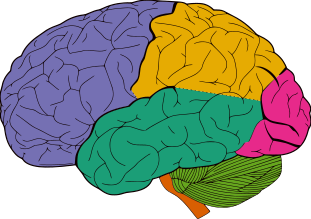
\includegraphics[height=3cm]{dev/wiki/brain_lobes.png}\url{https://en.wikipedia.org/wiki/Frontal_lobe}}
\hspace*{\fill}
\subcaptionbox{\label{fig:nerveFiber}}[.45\textwidth]{
\includegraphics[height=3cm]{dev/wiki/brain_fiber_paths.png}\url{https://en.wikipedia.org/wiki/Association_fiber}}
\hspace*{\fill}
\caption{(a) Illustration of human brain. (b) Illustration of a coronal human brain section. \itodo{a) name brain parts, redo in inkscape}}
\label{fig:human-fiber}
\end{figure}
% 
The frontal, parietal, temporal  and ocipital lobe (see \cref{fig:brainLobes}).
\\
The frontal lobe contains most of the ... functionalities.
The parietal lobe has \dummy{}
The ocipital lobe main function is the signal processing of the visual system.
The temporal lobes contain visual memories as well es auditry functions and language.
\par
The inner part of the brain also include cortival(? -> gm) structures like \dummy{}.
All this structures in the cerebellum and the cerebum contain on thir surfaces (outer as well as inner) a cortical (?) layer, which is filled with cell bodies.
This cells purpase are to process the information of all the signals comming from outside (and inside) the brain.
There are many types of cells involed in this process.
For example some can strengthen a signal or inhibite it.
In the human brain there are several (Billion?) cells which have a high interconnectivity in the local area as well as through the brain to different ...
This high coplex structure is the source of human intelligence, consisnes and much more.
Therefore it is a common goal of humanity to understand the human brain to improve medical treatment as well as \dummy{}.
% 
% \paragraph{Further information}
% This is only a short introduction into the brain architecture.
% It can be further seperated into much more objective parts as well as ...
% This is for example done via cell types and density research like the investigation of cortical layers.
% 
% 
% 
\section{Fiber Architecture} \label{sec:fiberArchitecture}
% 
\begin{figure}[!t]
\centering
\hspace*{\fill}
\tikzset{external/export next=false}
\subcaptionbox{\label{fig:coronalStained}BB 4201: Gray, White Matter, Coronal Section, Stained}[0.6\textwidth]{
\begin{tikzpicture}[]
    \node[inner sep=0pt, anchor = south west] (fig) at (0,0)
    {\includegraphics[width=0.6\textwidth]{dev/brain/BB_4201.png}};
    % \draw[] (0,0) grid (8,5);
    \draw[RED, ultra thick, <-] (5,4) -- ++ (-42:0.75) node[pos=1, anchor=north] {\textbf{WM}};
    \draw[GREEN, ultra thick, <-] (2.4,5) -- ++ (-65:0.75) node[pos=1, anchor=north] {\textbf{GM}};
\end{tikzpicture}
}
\hspace*{\fill}
\subcaptionbox{Cortical layers}[0.3\textwidth]{
\includegraphics[width=0.3\textwidth]{dev/wiki/layers.png}
}
\hspace*{\fill}
% 
\caption[GM, WM, layers]{}
\label{fig:BBrain}
\end{figure}
% 
% 
% 
\begin{figure}[!t]
\centering
% \subcaptionbox{\label{fig:headAndBrain}}[.28\textwidth]{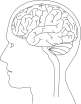
\includegraphics[height=3cm]{gfx/neuroanatomy/human-brain-profile.pdf}}
% \subcaptionbox{}[.42\textwidth]{\includegraphics[height=4cm]{gfx/neuroanatomy/human-brain-section.pdf}}\hfill
% \subcaptionbox{\label{fig:nerveFiber}}[.42\textwidth]{
\includegraphics[angle=90,width=0.75\textwidth,]{gfx/neuroanatomy/neuron-axon_.pdf}
% }
\caption{%(a) Illustration of human brain. 
% (a) Illustration of a coronal human brain section. (b)
Illustration of a neuron with axon and oligodendrocytes. The olegodendrocyte build up a layered lipid structure up, surrounding the axon. The myelin layers are separated along the axon by nodes of Ranvier. \itodo{name parts, ending of axon}}
\label{fig:human-brain}
\end{figure}
% 
Nerve cells are connected via different types of (nerve?) fibers.
A typical nerve cell (see \cref{fig:human-brain}) (if there is such a thing) has a cell body, which processes the incoming information.
The information arrives via dendrites, which are star like tree branches, which will connect to an incoming axon.
The axon is the main (and only) output of the cell.
It travels through the brain to its destination and connects there to a (maybe more or less random) brain cell.
This randomness is also part of the learning process in the brain.
After the brain axons are developed, no new axons are build anymore.
Only the strength of the signals and local structures changes as well as no used connections can be \say{deleted}.
Density of axons \dummy{}.
% Since there are (Billion?) of nerve cells, and there axons need to reach a specific target in a closed volume, the density of nerve fibers is quite high.
There diameter is around $\SI{0.5}{\micro\meter}$ up to several $\si{\micro\meter}$ (see \cref{tag:axonDiameter}).
The axon is surrounded by a myelin sheet, which is a lipid layered structure, build from near by olegodendrides.
These surroundings electric isolates the axon.
This improves the travelling speed of the electric action potential along the axon as well as its signal strength (voltage).
There are many different types of axons.
Some contain a very thick layer of myelin while others have none.
The high density of axons and myelin lets the brain where axons are located, white looking.
Therefore this structure of the brain gets its name \ac{WM}.
The outer cell bodies layer are called \ac{GM}.
In a nissle stained image, where the nerve cells are absorbing light, this is even more visible (see \cref{fig:coronalStained}).
\par
% 
% \begin{figure}[!t]
% 	\centering
% 	\includegraphics{gfx/neuroanatomy/human_wm_after_klinger_dissection.png}
% 	\caption{Electron microscopy image after klinger dissection \cite{destrieux:hal-01261930}. Fiber bundle structures are visible, following the same direction}
% % 	\label{fig:brain_sectioning}
% \end{figure}
% 
\begin{figure}[!t]
	\centering
	\subcaptionbox{}[.49\textwidth]{
	    \includegraphics[width=0.45\textwidth]{dev/brain/auto_seg_axon_0.png}}\hfill
    \subcaptionbox{}[.49\textwidth]{
        \includegraphics[width=0.45\textwidth]{dev/brain/auto_seg_axon_1.png}}
	\caption{Automatic segmentet nerve fiber tissue from an electron microscopy \cite{Abdollahzadeh2019}. }
% 	\label{fig:brain_sectioning}
\end{figure}
% 
Since this \ac{WM} has such a high density of fibers (up to billion in the corpus calosum) it is even under a microscope nearly impossible to investigate single fiber tracts through the brain.
One approach is a myelin staining (see \cref{fig:brainMyelinStain}).
Here nerve fibers which are myelinated are absorbing light (contrast).
Individual nerve fibers can be tracked inside the section.
However already for "smaller" nerve fiber bundles individual nerve fibers are lost.
Especially for dense white matter, no more information can be obtained.
It has also the disadvantage that no 3d orientation information can be easily mapped.
\Cref{fig:brainMyelinStain} shows a section with this technique inside the human thalamus.
It shows different kind of organisations of the nerve fibers.
Nerve fiber bundles are visible (orange) as well as net structures inside the \ac{GM}.
Latter are present to connect the nerve cells with each other inside the \ac{GM}, while the nerve fiber bundles let the axons reach there target area.
\par
% 
\todo{klinger section}
% 
\begin{figure}[!t]
	\centering
	\includegraphics{gfx/neuroanatomy/magic.png}
	\caption{Magic. TPFM auto fluorescence nerve fibers. Origin: \cite{Costantini2020}.}
	\label{fig:brainTPFM}
\end{figure}
% 
\begin{figure}[!t]
	\centering
	\tikzset{external/export next=false}
	\begin{tikzpicture}[]   
     \node[inner sep=0pt, anchor = south west] (fig) at (0,0)
       {\includegraphics[width=\textwidth]{gfx/neuroanatomy/NeuralNet-BrainAtlasDotOrg.png}};
     \draw[Orange, ultra thick] (7.65,6.15) ellipse (1 and 0.5);
     \draw[ProcessBlue, ultra thick] (10,4.5) ellipse (2 and 1);
     \draw[white, ultra thick] (0.5,0.5) -- ++ (0:1) node[pos=0.5, above] {\small $\SI{0}{\micro\meter}$};
    \end{tikzpicture}
% 	\includegraphics[width=\textwidth]{gfx/neuroanatomy/NeuralNet-BrainAtlasDotOrg.png}
	\caption{Myelin Staining. human thalamus, sagital section. \textcolor{Orange}{nerve fiber bundles}. \textcolor{ProcessBlue}{neural net}}
	\label{fig:brainMyelinStain}
\end{figure}
% 
Another tequnique is \ac{TPFM}. 
\cref{fig:brainTPFM} shows a measurement after \ac{3D-PLI} with the \ac{MAGIC} protocol.
This allows fluorescence measurments of the myelin which appears in \ac{3D-PLI} sections after PBS washing \cite{Costantini2021}.
The figure shows the 3d structure of (species, region).
In the lower left part of the volume \ac{WM} is present. 
The border between \ac{WM} and \ac{GM} is in the upper left to the lower right image.
In the upper right corner \ac{GM} is present with individual nerve fibers as well as nerve fiber bundles.
\par
% 
These exemplary data indicate the extreme complexity.
There are a lot more data available.
One comon teqchnique are electorn microscope data.
However the necesarry of a vacuum let the nerve fibers dry out and deform their structure significantly.
\par
% 
For different species with smaller brains, like rodents, imaging techniques like \textit{clearing} have a high potential and could already been used to map an (entire?) brain with axons.
However for a more complex and larger brain, this is up to this point not achieved.
Polarized light imaging, which uses the birefringence property of myelin, is a promising technique, already developed around the 1900, which allows to map the orientation of axons in a brain section.
This technique has, as all microscopic techniques which are using sections, the disadvantage, that the brain has to be cut and measured afterwards.
There are alternative methods like (OCT? \cite{Aumann2019}), which measures the brain section first, and then cuts the upper layer away, and measures the next section afterwards. It uses the reflection of the light than rather the transmitted light through the tissue.
However up to this point no entire large brain like a human brain was measured in its entirety.
Since \ac{3D-PLI} uses the already known sectioning techniques, which are developed since several decades, it can use this knowledge to its advantage.
% 
%
\section{Sectioning}
%
\begin{figure}[!t]
	\centering
    \setlength{\tikzwidth}{0.75\textwidth}
	\inputtikz{gfx/neuroanatomy/brain_sectioning}
	\caption{Illustration of sectioning. a)-b) block with imbedded brain, c) vibrating knife.}
	\label{fig:brain_sectioning}
\end{figure}
% 
For the cutting process, the tissue, \ie{} the brain, has to be frozen and imbedded into a solid material.
One commen material is parafine, however this is not possible for \ac{3D-PLI} \dummy[why?]{}.
For \ac{3D-PLI} it very is important, that the tissue does not build up crystal structures, because these are also birefringence.
Therefore the tissue is first ... into a ... liquid ...
After a time of a few months the tissue will then be frozen into a \SI{-70}{\degree}.
Then the frozen tissue can be fixated with a liquid glue on a cutting plate.
The glue is ...
It is also be used to build up a sourounding fixating material to stabilize the brain in the cutting process.
Additionally markers are fixed which help in the later registration process, which will align the tissue sections in a 3d volume again \cite{Schober2016,Ali2018,Schmitz2018}.
\par
The cutting is done in a microtome (see \cref{fig:brain_sectioning}).
In there the temperature can be held at about \SI{-70}{\degree} and allows no heating of the tissue.
The brain is moved against a vibrating very sharp knife.
This allows for the thin sectioning of about \SI{60}{\micro\meter}.
After the cutting, the tissue is put onto a glass specimen.
Since the tissue is such thin and filigran, it is not always possible to avoid cracks for example.
This also will be as best as possible corrected in the registration process.
The tissue will be ... with a glycerin ... and finally siled with another glass.
To prevent the formation of waves in the tissue, the glass is weighted.
The tissue sections are then stored into a refrigerator at \SI{-70}{\degree\celsius}.
The tissue can then finally be measured in the \ac{3D-PLI} microscopes (see \cref{sec:expSetup} for further techniqule informations).
% 
% 
\section{Axon Literature}
\label{microscopy}
% 
Axon diameter \cite{Liewald2014}:
% 
\begin{table}[!b]
\centering
\pgfplotstabletypeset[
thesisTableStyle,
font=\footnotesize,
col sep=comma,
columns/Name/.style={string type},
columns/Mean/.style={fixed zerofill},
columns/SD/.style={fixed zerofill},
columns/Median/.style={fixed zerofill},
columns/Max/.style={fixed zerofill},
columns/Min/.style={fixed zerofill},
columns/n/.style={dec sep align},
rowbf={1},rowbf={8},rowbf={19},
rowem={2},rowem={5},
rowem={9},rowem={12},rowem={15},
rowem={20},rowem={23},rowem={26},
]{data/axon_distribution.csv}
\caption{axon diameter distribution of the human brain in \si{\micro\meter} \cite{Liewald2014}}
\label{tag:axonDiameter}
\end{table}
% 
\begin{table}[!b]
\centering
\pgfplotstabletypeset[
thesisTableStyle,
font=\footnotesize,
col sep=semicolon,
columns={article,cite,gratio},
columns/article/.style={string type, column name=name, column type = {l}},
columns/cite/.style={string type, column name=cite, column type = {l}},
columns/gratio/.style={string type, column name=$g_{\mathit{ratio}}$},
]{data/gratio.csv}
\caption{human $g_{\mathit{ratio}}$ from invivo mri studies.}
\label{tab:gratio}
\end{table}
% 
axon = 0.5-1.0 diameter (most frequent
thickness of myelin mean = 0.09, median 0.08
-> g-ratio 0.9 (electron microscop, upper boundry)
% 
g-ratio
\cite{Cercignani2017} -> 0.65-0.8 mrt, healty male and female different age, different regions\\
\cite{FitzGibbon2013} -> 0.58-0.84 (Retina), electron microscopy
% 
\itodo{brechungsindex}
% 
% \begin{figure}[!t]
% 	\centering
% 	 \includegraphics[clip, trim=0.65cm 6.25cm 0.4cm 0.5cm]{gfx/neuroanatomy/nature_3d_em_optical_nerve.png}
% 	\caption{\dummy{only show a} Three dimensional electron microscopy reveals changing axonal and myelin morphology along normal and partially injured (*, light green) optic nerves. Origin: \cite{Giacci2018} (reative Commons Attribution 4.0 International License).}
% % 	\label{fig:brain_sectioning}
% \end{figure}
%
% 
\cleardoublepage
\setcounter{chapter}{2}
\chapter{Theory}
\label{sec:theory}
% 
\cleanchapterquote{The first principle is that you must not fool yourself and you are the easiest person to fool.}{Richard P. Feynman}{}%\newline
%
\section{Introduction}
The following section lists the physical theories needed to describe the mathematics behind \ac{3D-PLI}. This includes the basic properties of light with the description of their polarization state, the optical models of the tissue, i.e. the nerve fibers and the mathematical description of the experimental setup of \ac{3D-PLI}. The first part of this chapter was written with the help of \cite{demtroeder2, Fliebach2012}.
% 
% 
% 
\section{Electromagnetic Wave}
% 
Light is an electromagnetic wave. Electromagnetism is first fully described by James Clerk Maxwell. He formulated the Maxwell-Equations \cref{eq::maxwell_general}, generalized from the previous work of Johann Carl Friedrich Gau{\ss}, Michael Faraday and Andr\'{e}-Marie Amp\`{e}re and others. 
% 
% \begin{align} 
% \begin{split} \label{eq::maxwell_macro}
%     \nabla \cdot \vec{D} &= 4\pi\rho_\text{f}\\
%     \nabla \cdot \vec{B} &= 0\\
%     \nabla \times \vec{E} &= -\frac{1}{c} \frac{\partial \vec{B}} {\partial t}\\
%     \nabla \times \vec{H} &= \frac{1}{c} \left(4\pi\vec{J}_\text{f} + \frac{\partial \vec{D}} {\partial t} \right)
% \end{split}
% \end{align}
% 
\begin{align} 
\begin{split} \label{eq::maxwell_general}
    \nabla \cdot \vec{E} &= \frac {\rho} {\varepsilon_0}\\
    \nabla \cdot \vec{B} &= 0\\
    \nabla \times \vec{E} &= -\frac{\partial \vec{B}} {\partial t}\\
    \nabla \times \vec{B} &= \mu_0\left(\vec{j} + \varepsilon_0 \frac{\partial \vec{E}} {\partial t} \right)
\end{split}
\end{align}
% 
with $\nabla \coloneqq \left({\frac{\partial}{\partial x}}, {\frac{\partial}{\partial y}}, {\frac{\partial}{\partial z}} \right)$ as vector differential operator, $\vec{E}$ as eletric field, $\rho$ as electric charge density, $\varepsilon_0$ as permittivity of free space, $\vec{B}$ as magnetic field, $\mu_0$ as permeability of free space and $\vec{j}$ as electric current density.
% 
The first equation states no electric field can be generated without an electric charge (charge conservation).
The second equation states, magnetic monopoles does not exists. The basic entity of an magnetic field is a dipole.
The third and forth equation show the interconnection of the electric and magnetic fields in space and time. A change in the electric field yields to a magnetic field and vice versa. Equation forth additional indicates the creation of a magnetic field from a electric current. The maxwell equation fullfill the continoiut ... $\divergence j + \frac{\partial \rho}{\partial t} = 0$
% 
In a vacuum this simplifies with $\rho = 0$ and $\vec{J} = \vec{0}$ to:
% 
\begin{align}
\begin{split} \label{eq::maxwell_vacuum}
  \nabla \cdot \vec{E} &= 0 \quad\\
  \nabla \cdot \vec{B} &= 0 \quad\\
  \nabla \times \vec{E} &= -\frac{\partial\vec B}{\partial t}\\
  \nabla \times \vec{B} &= \mu_0\varepsilon_0 \frac{\partial\vec E}{\partial t}
  \end{split}
\end{align}
% 
With 
\begin{align}
\begin{split} 
    \nabla \times \nabla \times \vec{E} = -\nabla \times \frac{\partial \vec{B}} {\partial t} &= -\frac{\partial} {\partial t} \left( \nabla \times  \vec{B} \right)\\
    &= -\varepsilon_0 \cdot \mu_0 \frac{\partial^2 \vec{E}}{\partial t^2}
\end{split}
\end{align}
% 
the identity $\nabla \times \left( \nabla \times \vec{A} \right) = \nabla(\nabla \cdot \vec{A}) - \nabla^{2}\vec{A}$ and $\mu_0\varepsilon_0 = \frac{1}{c^2}$, with $c$ as the speed of light\footnote{can be derived from Maxwells equation and Lorentz force in a vacuum}, this further simplifies to:
% 
\begin{align}
\begin{split} \label[pluralequation]{eq::maxwell_wave_equations}
  \frac{1}{c^2} \frac{\partial^2 \vec{E}}{\partial t^2} - \nabla^2 \vec{E} &= 0 \\
  \frac{1}{c^2} \frac{\partial^2 \vec{B}}{\partial t^2} - \nabla^2 \vec{B} &= 0
\end{split}
\end{align}
% 
Another common representation is
% 
\begin{align}
\begin{split} \label{eq::maxwell_wave_equations_box}
  \Box \ \vec{E} &= 0 \\
  \Box \ \vec{B} &= 0
\end{split}
\end{align}
% 
with the help of the d'Alembert operator $\Box \coloneqq \partial^a\partial_a = \nabla^2 - \frac{1}{c^2} \frac{\partial^2}{\partial t^2}$.
% 
This also shows $c^2  \frac{\partial B} {\partial z} = \frac{\partial E}{\partial t} \Rightarrow \vec{E} \cdot \vec{B} = 0$ that the electric and magnetic field components are perpendicular to each other.
% 
\subsection{Solving MW Equ in vacuum}
% 
\Cref{eq::maxwell_wave_equations} have the shape of a wave equation and can therefore as known be solved by
% 
% Using the Maxwell equation in vacuum \ref{eq::maxwell_vacuum}, one can find the most simple solution to the differential equation is a wave:
% 
\begin{align}
\begin{split} \label{eq::dgl_solution}
  \vec{E}( \vec{r}, t ) &= g(\phi( \vec{r}, t )) = g( \omega t - \vec{k} \cdot \vec{r} + \varphi)\\
  \vec{B}( \vec{r}, t ) &= g(\phi( \vec{r}, t )) = g( \omega t - \vec{k} \cdot \vec{r} + \varphi )
\end{split}
\end{align}
% 
where $g$ is any well behaved function and therefore also their superposition.
% 
With the help of
% 
\begin{align}
k = \mathopen| \vec{k} \mathclose| = \frac{\omega}{c} =  \frac{2 \pi}{\lambda}
\end{align}
% 
a planar wave can be descriped by
% 
\begin{align}
\begin{split} \label{eq::plane_wave}
\vec{E}(\vec{r}) &= \vec{E}_0 \cdot e^{ -i \, \vec{k} \cdot \vec{r} }\\
 \vec{B}(\vec{r}) &= \vec{B}_0 \cdot e^{ -i \, \vec{k} \cdot \vec{r} }
\end{split}
\end{align}
% 
% 
% 
\subsection{Polarization}
% 
\begin{figure}[!t]
\centering
\setlength{\tikzwidth}{\textwidth}
\inputtikz{gfx/pli/polarization_state}
\label{fig:polarization_state}
\caption{Illustration of light polarization state.}
\end{figure}
% 
This shows, that the light wave travels in direction of $\vec{k}$ (no it does not, you have to show, that k is perpendicular to E and B).
Therefore the light has a property called polarization.
Polarization is the direction of the, usually, electric field component.
% 
A superposition of x and y wave with z equal to direction of propagation yield to the general form
\begin{align}
\vec{E}(z,t) &= \begin{pmatrix} E_{0x} \cdot e^{ -i \phi_x } \\ E_{0y} \cdot e^{ -i \phi_y } \\ 0 \end{pmatrix}
e^{ -i (kz - \omega t)}
\end{align}
%
\begin{figure}[!t]
\centering
\tikzset{external/export=false}
{
% \captionsetup[sub]{textfont=normalsize}
\captionsetup[sub]{position=top, skip=-14pt}
\tikzset{>=stealth}
\tikzset{cross/.pic={
\draw[->] (-{sqrt(2)},0) -- ({sqrt(2)},0) node[anchor=north]{\footnotesize $E_x$};
\draw[->] (0,-{sqrt(2)}) -- (0,{sqrt(2)}) node[anchor=east]{\footnotesize $E_y$};
}}
% 
\subcaptionbox{}[.3\textwidth]{
\begin{tikzpicture}
\pic at (0,0) {cross};
\draw[] (0, 2) node () {linear, horizontal};
\draw[thick, arrows={Stealth[scale=1]-Stealth[scale=1]}] (-1, 0) -- (1, 0);
\draw[] (0, -2) node () {$\begin{pmatrix} 1&0 \end{pmatrix}$};
\draw[] (0, -3) node () {$\begin{pmatrix} 1&1&0&0 \end{pmatrix}$};
\end{tikzpicture}
}
\subcaptionbox{}[.3\textwidth]{
\begin{tikzpicture}
\pic at (0,0) {cross};
\draw[] (0, 2) node () {linear, vertical};
\draw[thick, arrows={Stealth[scale=1]-Stealth[scale=1]}] (0, -1) -- (0, 1);
\draw[] (0, -2) node () {$\begin{pmatrix} 0&1 \end{pmatrix}$};
\draw[] (0, -3) node () {$\begin{pmatrix} 1&-1&0&0 \end{pmatrix}$};
\end{tikzpicture}
}
\subcaptionbox{}[.3\textwidth]{
\begin{tikzpicture}
\pic at (0,0) {cross};
\draw[] (0, 2) node () {linear, $\pi/4$};
\draw[thick, arrows={Stealth[scale=1]-Stealth[scale=1]}] (-1, -1) -- (1, 1);
\draw[] (0, -2) node () {$\begin{pmatrix} 1&1 \end{pmatrix}$};
\draw[] (0, -3) node () {$\begin{pmatrix} 1&0&1&0 \end{pmatrix}$};
\end{tikzpicture}
}
\\[2em]
\subcaptionbox{}[.3\textwidth]{
\begin{tikzpicture}
\pic at (0,0) {cross};
\draw[] (0, 2) node () {left circular};
\draw[thick] plot[domain=0:360,samples=90,smooth] ({cos(\x)},{sin(\x)});
\draw[thick, arrows={-Stealth[scale=1]}] plot[domain=44:45,samples=1] ({cos(\x)},{sin(\x)});
\draw[thick, arrows={-Stealth[scale=1]}] plot[domain=224:225,samples=1] ({cos(\x)},{sin(\x)});
\draw[] (0, -2) node () {$\begin{pmatrix} 1&i \end{pmatrix}$};
\draw[] (0, -3) node () {$\begin{pmatrix} 1&0&0&-1 \end{pmatrix}$};
\end{tikzpicture}
}
\subcaptionbox{}[.3\textwidth]{
\begin{tikzpicture}
\pic at (0,0) {cross};
\draw[] (0, 2) node () {right circular};
\draw[thick] plot[domain=0:360,samples=90,smooth] ({cos(\x)},{sin(\x)});
\draw[thick, arrows={-Stealth[scale=1]}] plot[domain=46:45,samples=1] ({cos(\x)},{sin(\x)});
\draw[thick, arrows={-Stealth[scale=1]}] plot[domain=226:225,samples=1] ({cos(\x)},{sin(\x)});
\draw[] (0, -2) node () {$\begin{pmatrix} 1&-i \end{pmatrix}$};
\draw[] (0, -3) node () {$\begin{pmatrix} 1&0&0&1 \end{pmatrix}$};
\end{tikzpicture}
}
\subcaptionbox{}[.3\textwidth]{
\begin{tikzpicture}
\pic at (0,0) {cross};
\draw[] (0, 2) node () {unpolarized};
\draw[] (0, -3) node () {$\begin{pmatrix} 1&0&0&0 \end{pmatrix}$};
\end{tikzpicture}
}
}
\caption{polarization states, check vector length,\itodo{test speed}} 
\label{fig:polarization_state_vectors}
\end{figure}
%
\Cref{fig:polarization_state_vectors} shows another representation of the polarization sate of a light wave.
It show the component perpendicular to the travelling direction.
Therefore the time variation can be shown on the xy-plane.
Additionally the states can be describe by the Jones or Stokes calculus, later described in \cref{sec:jones,,sec:mueller_stokes}.
% 
% 
% 
\subsection{Light in medium}
% 
The maxwell equations in ... are described above. They can be solved analog to ... . This yields to some special behavier, \eg{} the magnetic and electic field component get out of phase.
However here only the two properties of absorptiona and difraction are described.
They derivation can be found \eg{} \cite{demtroeder2, Fliebach2012}.
% 
\subsection{Absorption}
% 
\begin{align}
    I = I_0 \exp(-\mu x)
\end{align}
% 
Beersche law of absorption with $\mu = \frac{4\pi \kappa}{\lambda_0}$ where $\kappa$ is the imaginary part of the complex refractive index.
% 
\subsection{Refraction}
% 
\begin{figure}[!t]
\centering
\setlength{\tikzwidth}{\textwidth}
\inputtikz{gfx/pli/refraction}
\label{fig:optic_refraction}
\caption{Illustration of refraction.}
\end{figure}
% 
Refraction is the property of light to change direction as it passes from one medium to another. This can be shown by using the full Maxwell equations  for non-conductive material, \ie{} $\vec{j} = 0, \rho = 0$, that the dgl consit out of a primary wave with from atomic medim induced secundary waves, which leads to a reduction of the velocity of the resulting wave. Mathematically this can be described by a complex number $n = c' / c$.
Using this relationship at a boundary surface between two media, one can show that the incident light beam splits into a reflecting and transmittang light wave. The reflecting light wave has the same angle as the incident light beam relativ the the surface normal. The transmitting light beam however due to the reduction of the velocity, changes its direction described by the snellius ...
\begin{align}
    n_0 \sin \alpha = n_1 \sin \beta
\end{align}

% 
\begin{align}
\underline{n} = n + i\kappa
\end{align}
% 
\begin{align}
\begin{split}
\vec{E}(z, t) &= \operatorname{Re}\! \left[\vec{E}_0 \cdot e^{i\, (kz - \omega t)}\right] \\
&= \operatorname{Re}\! \left[\vec{E}_0 \cdot e^{i\, (2\pi(n + i\kappa)z/\lambda_0 - \omega t)}\right] \\
&= e^{-2\pi \kappa z/\lambda_0} \operatorname{Re}\! \left[\vec{E}_0 \cdot e^{i\, (kz - \omega t)}\right]
\end{split}
\end{align}
% 
% 
% 
\subsection{Birefingence}
%
\begin{figure}[!t]
\centering
\setlength{\tikzwidth}{\textwidth}
\inputtikz{gfx/pli/retardation}
\caption{Illustration of retardation.}
\label{fig:optic_retardation}
\end{figure}
% 
\begin{figure}[!t]
\centering
\subcaptionbox{}[.49\textwidth]{
\setlength{\tikzwidth}{0.49\textwidth}
\inputtikz{gfx/pli/ellipsoid_a}}
\subcaptionbox{}[.49\textwidth]{
\setlength{\tikzwidth}{0.49\textwidth}
\inputtikz{gfx/pli/ellipsoid_b}}
\caption{birefringence elipsoid}
\label{fig:index_elipsoid}
\end{figure}
% 
Material can have a different refractive index depending on the relative orientation and polarization of the light beam.
This property is known as birefringence.
The refractive index can be described as the refractive index $n_o$ and extraordinary  $n_e$.
Since these two are perpendicular to each other, one can split the light beam into the same perpendicular parts and describe each by its own.
These two light beams, except for the trivial case of a light beam is perpendicular to the surfave, have a different direction.
However for small relative length (hängt von n ab, bzw der phasenänderung) the two light beams leave the material at the same point and recombined at the end.
The change of phase is called birefringence and is described by the difference between the .. and ...
% 
\begin{align}
    \Delta n = n_e - n_o \> .
\end{align}
% 
This .. can be visualized by the index ellipsoid \cref{fig:index_elipsoid}.
The change of the amplitude and phase can be described by the following techniques.
% 
% 
% 
\subsection{Jones}
\label{sec:jones}
% 
The Jones calculus, introduced by Robert Clark Jones in 1941, describes the polarization state of a light beam by a complex vector $J$:
% 
\begin{align}
    \vec{J} = \begin{pmatrix} E_x \exp(i \phi_x) \\ E_y \exp(i \phi_y) \end{pmatrix}
\end{align}
% 
The amplitude of the perpendicular components are $E_x$ and $E_y$ with their phase $\phi_x$ and $\phi_y$.
Optical elements, which changes the polarization state, such as a polarization filter and retarder, can be desribed by a matrix:
% 
\begin{align}
\begin{split}
\mat{P}_x = 
\begin{pmatrix}
1 & 0 \\ 0 & 0
\end{pmatrix}
, \,
\mat{P}_y = 
\begin{pmatrix}
0 & 0 \\ 0 & 1
\end{pmatrix}
, \,
\mat{M} =
\begin{pmatrix}
e^{i \varphi_x} & 0 \\ 0 & e^{i \varphi_y}
\end{pmatrix}
, \,
\Lambda_{1/4}=
e^{\frac{i \pi}{4}}
\begin{pmatrix}
1 & 0 \\ 0 & -i
\end{pmatrix}
\end{split}
\end{align}
% 
A rotation of the axis can be achieved by a 2d rotation matrix $\mat{R}$:
% 
\begin{align}
\begin{split}
\mat{M}(\theta )=\mat{R}(\theta )\cdot\mat{M}\cdot\mat{R}(-\theta )
, \>
\mat{R}(\theta ) = 
\begin{pmatrix}
\cos \theta & -\sin \theta \\
\sin \theta & \cos \theta
\end{pmatrix}
\end{split}
\end{align}
% 
% 
% 
\subsection{M\"uller-Stokes}\label{sec:Mueller-Stokes}
\label{sec:mueller_stokes}
% 
Analog to \cref{sec:jones} the M\"uller-Stokes formalism, described by George Gabriel Stokes in 1852, also describes the polarication state of a light beam.
However it does not use the absolute .. but the relative polarication between both components:
% 
\paragraph{Stokes vector}
\begin{align}
\begin{split}
S_0 &= I \\
S_1 &= I p \cos 2\psi \cos 2\chi \\
S_2 &= I p \sin 2\psi \cos 2\chi \\
S_3 &= I p \sin 2\chi
\end{split} \hspace{-6em}
\begin{split}
& \equiv \langle E_x^{2} \rangle + \langle E_y^{2} \rangle \\
%  & = \langle E_a^{2} \rangle + \langle E_b^{2} \rangle \\
%  & =  \langle E_l^{2} \rangle + \langle E_r^{2} \rangle \\
& \equiv \langle E_x^{2} \rangle - \langle E_y^{2} \rangle \\
& \equiv \langle E_a^{2} \rangle - \langle E_b^{2} \rangle \\
& \equiv  \langle E_l^{2} \rangle - \langle E_r^{2} \rangle
\end{split}
, \,
\vec{S} =
\begin{pmatrix} S_0 \\ S_1 \\ S_2 \\ S_3\end{pmatrix}
\end{align}
% 
% \begin{align}
% \begin{split}
% S_0 & \equiv \langle E_x^{2} \rangle + \langle E_y^{2} \rangle \\
%  & = \langle E_a^{2} \rangle + \langle E_b^{2} \rangle \\
%  & =  \langle E_l^{2} \rangle + \langle E_r^{2} \rangle \\
% S_1 & \equiv \langle E_x^{2} \rangle - \langle E_y^{2} \rangle \\
% S_2 & \equiv \langle E_a^{2} \rangle - \langle E_b^{2} \rangle \\
% S_3 & \equiv  \langle E_l^{2} \rangle - \langle E_r^{2} \rangle
% \end{split}
% \end{align}
% 
Therefore the phase can not be described anymore.
However the relative phase information is stored and can be used to describe also polarization states of polarization filters, which can not be described by Jones.
Aanlog to Jones one can formulate the matrices for the optical components:
% 
\paragraph{Linear Polarizer}
\begin{align}
\mat{P}_x=\frac{1}{2}
\begin{pmatrix}
    1 & 1 & 0 & 0 \\
    1 & 1 & 0 & 0 \\
    0 & 0 & 0 & 0 \\
    0 & 0 & 0 & 0
  \end{pmatrix}
, \,
\mat{P}_y=\frac{1}{2}
\begin{pmatrix}
     1 & -1 & 0 & 0 \\
    -1 &  1 & 0 & 0 \\
     0 &  0 & 0 & 0 \\
     0 &  0 & 0 & 0
\end{pmatrix}
\end{align}
% 
\paragraph{retarder}
\begin{align}
\mat{M}=\
\begin{pmatrix}
    1 & 0 & 0 &  0 \\
    0 & 1 & 0 &  0 \\
    0 & 0 & \cos \delta & \sin \delta \\
    0 & 0 & -\sin \delta &  \cos \delta
\end{pmatrix}
\end{align}
% 
\paragraph{Quarter-wave plate (fast-axis vertical)}
\begin{align}
\Lambda_{1/4}=\
\begin{pmatrix}
    1 & 0 & 0 &  0 \\
    0 & 1 & 0 &  0 \\
    0 & 0 & 0 & -1 \\
    0 & 0 & 1 &  0
\end{pmatrix}
\end{align}
% 
\paragraph{Rotation Matrix}
\begin{align}
\mat{R}(\theta)=
\begin{split}
\begin{pmatrix}
    1 &                0 &               0 & 0 \\
    0 & \cos{(2\theta)} & -\sin{(2\theta)} & 0 \\
    0 & \sin{(2\theta)} & \cos{(2\theta)} & 0 \\
    0 &                0 &               0 & 1
  \end{pmatrix}
\end{split}
\end{align}
% 
% \paragraph{Rotation Matrix}
% \begin{align}
% \frac{1}{2}
% \begin{pmatrix}
%     1 &                0 &               0 & 0 \\
%     0 &  \cos{(2\theta)} & \sin{(2\theta)} & 0 \\
%     0 & -\sin{(2\theta)} & \cos{(2\theta)} & 0 \\
%     0 &                0 &               0 & 1
% \end{pmatrix}
% \end{align}
\todo{matrix multi}
% 
% \section{Tissue Discretization}
% % 
% By deviding the volume into small diskreticed subvolumes, one can multiply the .. all together and ... (analog Riemann sum)
% \begin{align}
%     \int F \, dt \approx \sum_n F \, \Delta t
% \end{align}
% see simulation?
% 
%  see simulation
% \paragraph{Micro vs Macro:}
% % 
% % \begin{align}
% %   \int_{y_\textit{min}}^{y_\textit{max}} \vec{v}(y) \,dy\\
% %   x = const
% %   y = y(\alpha,x) = tan(\alpha) \cdot x\\
% %   \vec{v}_r = \begin{pmatrix} \cos(\alpha)\\ \sin(\alpha)\\0\end{pmatrix}, \, \vec{v}_p = \begin{pmatrix} 0\\ 0\\1\end{pmatrix}\\
% %   \vec{v}_r = \begin{pmatrix} \cos(\arctan(y/x))\\ \sin(\arctan(y/x))\\0\end{pmatrix}\\
% %   \int_{y_\textit{min}}^{y_\textit{max}} \vec{v}_p(y) \,dy = (y_\textit{max} - y_\textit{min}) \cdot e_z\\
% %   \int_{y_\textit{min}}^{y_\textit{max}} \vec{v}_r(y) \,dy = \int_{y_\textit{min}}^{y_\textit{max}} \cos(\arctan(y/x)) dy \cdot e_x \\
% %   = x\left(\sinh^{-1}(y_\textit{max}/x) - \sinh^{-1}(y_\textit{min}/x)\right) \\
% %   = 2x \left(\sinh^{-1}\left(\frac{2\sqrt{R-x^2}}{x}\right)\right)
% % \end{align}
% % 
% % \begin{align}
% %     % \frac{\oint \vec{v}_z \mathrm{d}A}{\oint \vec{v}_x \mathrm{d}A} = 
% %     % \frac{\int_{-1}^{1}\abs{\vec{v}} \mathrm{d}x}{\int_{-\frac{\pi}{2}}^{\frac{\pi}{2}} \abs{\vec{v}} \cos(\varphi) \mathrm{d}\varphi} =
% %     % \frac{2}{1}
% %     \frac{A_{\Box}}{A_{\circ}} = \frac{4}{\pi}
% % \end{align}
% % 
% \todo{why 2*dn?}
% 
\section{Experimental Setup}\label{sec:expSetup}
%
\begin{figure}[!t]
    \captionsetup[sub]{position=top}
    \setlength{\tikzwidth}{\textwidth}
	\centering
	\subcaptionbox{\label{setup-lap} \ac{LAP}}[\textwidth]{
% 		\resizebox{0.95\textwidth}{!}{
		\inputtikz{gfx/pli/pli_setup}
% 	}
	}\\
	\subcaptionbox{\label{setup-pm} \ac{PM}}[\textwidth]{
% 		\resizebox{0.95\textwidth}{!}{
		\inputtikz{gfx/pli/pli_setup_pm}
% 	}
	}
	\caption{Illustration of PLI setup.}
	\label{fig:pli_setup}
\end{figure}
%
\begin{figure}[!t]
    % \captionsetup[sub]{position=top}
    \setlength{\tikzwidth}{0.3\textwidth}
	\centering
	\subcaptionbox{\ac{LAP}}[.49\textwidth]{
			\inputtikz{gfx/pli/pli_detail}}\hfill
	\subcaptionbox{\ac{PM}}[.49\textwidth]{
			\inputtikz{gfx/pli/pli_detail_pm}}
	\caption{Illustration of detail PLI setup.}
	\label{fig:pli_detail}
\end{figure}
%
The \ac{3D-PLI} setup is described in \cite{Axer2011} with the tiltable light beam microscope (LMP) in \cite{Wiese:887678}.
For the routine measurements two (three) microscope systems are currently in use.
The first use of a high throughput microscope is the \ac{LAP} with a pixel size of about \SI{60}{\micro\meter}. \footnote{can be change by the optic also to $\SI{40}{\micro\meter}$ and $\SI{20}{\micro\meter}$, but remains for the routine measurements with $\SI{60}{\micro\meter}$.}
It consist out of a led light source (\SI{525}{\nano\meter}), a rotatable polarization filter, a rotatable quarter wave retarder, the specimen stage, which can be tilted for oblique views, a rotatable polarizer.
Both polarizer and quarter wave retarder are rotated at the same time.
The both polarizers have a phase offset of $\SI{90}{\degree}$, the first polarizer and the quarter wave retarder of $\SI{45}{\degree}$ (see (see \cref{setup-lap}).
The second system \ac{LMP3D} microscope fullfills the same measurments, however the retarder is placed after the tissue specimen and fixed with the polarizer without any rotations (see \cref{setup-pm}).
Mathematically it measures the same signal.
\footnote{The rotatable filters of the \ac{LAP} has the advantage, that noise like dust particles can be easy identified and removed. Since the microscop is in a more confined "box" this is not necesarry.}
A difference is that the optical path is in reverse to the \ac{LAP} system.
Since there is a mirror in the path, the image is flipped again so that the coordinate systems stays the same (see \cref{fig:pli_detail}).
% 
\subsection{Signal}
% 
From the M\"{u}ller Matrices (\cref{sec:Mueller-Stokes}) as shown in \cite{MenzelMaster,MenzelDissertation}, that the intensity signal, measured by the \ac{CCD}-sensor, follows a sinusiodal curve:
% 
% \begin{align}
% I = \underbrace{\frac{I_0}{2}}_{\mathclap{\mathit{transmittance}}}
%     \bigl[ \sin\bigl(2\rho - 2{\underbrace{\vphantom{\frac{I_0}{2}} \varphi}_{\mathclap{\mathit{direction}}}} \bigr)
%     \cdot \sin \bigl( {\underbrace{\vphantom{\frac{I_0}{2}} 2\pi\frac{d \dn}{\lambda} \cos^2\left( \alpha \right)}_{\mathclap{\delta \, \coloneqq \, \mathit{retardation}}}} \bigr) \bigr]
% \end{align}
\begin{align}
\label{eq:pli_signal}
\begin{split}
I =\frac{I_0}{2}\bigl[ \sin\bigl(2\rho - 2\varphi \bigr)\cdot \sin \bigl( 2\pi\frac{d \dn}{\lambda} \cos^2\left( \alpha \right) \bigr) \bigr] \\
\text{with} \enspace \delta \coloneqq 2\pi\frac{d \dn}{\lambda} \cos^2\left( \alpha \right) \enspace 
\text{and} \enspace \trel \coloneqq \frac{d \dn}{\lambda}
\end{split}
\end{align}
% 
Since \cref{eq:pli_signal} describes a sinosoidal signal, the fourier analysis is a obvious choise.
For a discrete, aquidistant measurement of the rotation angles $\rho$, one can use the fourier series with the three coefficients to describe the signal:
% 
% \begin{align}
% \begin{split}
% A \sin(\omega t + \alpha) + B \sin(\omega t + \beta) &= \sqrt{C^2 + D^2} \cdot \sin \, \left( \omega t + \tan^{-1} \left( \frac{D}{C} \right) \right)
% \end{split}
% \\
% \begin{split}
% C &= A \cos(\alpha)+ B \cos(\beta)\\
% D &= A \sin(\alpha)+ B \sin(\beta)
% \end{split} \nonumber 
% \end{align}

\begin{align}
\begin{split}
\rho &= [\SI{0}{\degree}, \frac{1\cdot180}{N+1}\si{\degree}, \frac{2\cdot180}{N+1}\si{\degree}, ..., \frac{N\cdot180}{N+1}\si{\degree}]\\
a_0 &= \frac{1}{N} \sum(\mathit{data})\\
a_1 &= \frac{2}{N} \sum(\mathit{data} \cdot \sin(2 \cdot \rho)\\
b_1 &= \frac{2}{N} \sum(\mathit{data} \cdot \cos(2 \cdot \rho)
\end{split}
\end{align}

With these the final \ac{3D-PLI} modalities are calculated:

\begin{align}
\begin{split}
\mathit{transmittance} &= 2 \cdot a_0\\
\mathit{direction} &= 0.5 \cdot \atantwo(-b_1 / a_1)\\
\mathit{retardation} &= \frac{\sqrt{a_1^2 + b_1^2}}{a_0}
\end{split}
\end{align}



% 
\subsection{Tilted signal}
% 
To be able to analyse the inclination $\alpha$ one has to distiguish the relative strength of the birefringence from the $\cos^2(\alpha)$.
For this purpose a tiltable specimen was developed, which allows measuring the light signal through the tissue with a different angle of incidenc.
This mean, that tissue and therefore the nerve fibers also change their orientation by the tilting angles $\theta, \varphi$.
Additionally the distance the light travels through the tissue, elongigates by $1/\cos(\theta)$ \cref{fig:tilted_side_view}.
% 
Depending on the \pixelsize{}, in the case of the \ac{LAP} system, this light travels though the same volume, but with another orientation.
Therefore a measurement of multiple light paths can be ... and the resulting signals can be used to analyse the inclination and relative birefrigente tissue thickness \trel{}.
In the case of a tiltible specimen, the angle of incidence on the glass ... and the tissue also changes the angle of the light by snellius law.
All angles mentiont here are if not specified always the change of angle of the light inside the tissue (see \cref{fig:tilting_camera_view}). 
This also leads to a perspective shift, which has to be corrected by a registration process.
In this case an affine transformation.
% 
In \cite{Schmitz2018} this analys published under the name of \ac{ROFL}, which builds up on the work of \cite{Wiese:887678}.
The idea is to fit the measured signals of all light paths simultaniously.
Because the change of signal is proportional to the $\cos(\alpha)$ this however means, that for steep fibers, the changes are not only small, but also the amplitude of the signal is very small.
This leads to the problem of increasing uncertanty with increasing inclination angle.
\\
A further problem is that for a smaller \pixelsize{} the light path cannot be neglected anymore.
For the \ac{LMP3D} system this means, that with a maximal tilting angle of about $\SI{3}{\degree}$ and a usually tissue thickness of $\SI{60}{\micro\meter}$ the light path is measured in n pixels away from the non tilting case, if the rotation point is in the center of the tissue.
\\
However for homoginoius tissue, like the \ac{WM} may be some regions, the analysis technique can still be applied.
A change in density, orientation or dispersion however will lead to a false result.
% 
% 
% 
\section{Orientation}
% 
\begin{figure}[!t]
\centering
\setlength{\tikzwidth}{0.4\textwidth}
\begin{center}
\begin{tabular}{m{6cm}m{6cm}}
\includegraphics[width=\tikzwidth]{gfx/pli/color_sphere.png}
&
\inputtikz{gfx/pli/hsv_sphere}
\\
\begin{minipage}[t]{0.42\textwidth}
\leavevmode\subcaption{2d hsv sphere}
\end{minipage}
&
\begin{minipage}[t]{0.42\textwidth}
\leavevmode\subcaption{\label{fig:sphere}3d hsv sphere}
\end{minipage}
\end{tabular}
\end{center}
% 
\vspace{-1em} % because of tabular?
\caption{collor spheres}
\label{fig:spheres}
\end{figure}
% 
% 
The orientation of the birefringence axis is descibed by the direction angle $\varphi$ and inclination angle $\alpha$ (see \cref{fig:sphere}).
To be able to show a 3d information, the \textit{hsv-black} is usually shown in \ac{3D-PLI}.
It color code the orientation by:
\begin{align}
\begin{split}
    H &= \varphi/\pi\\
    S &= 1\\
    V &= 1-\alpha / \pi/2
\end{split}
\end{align}
This way the color corresponds to the direction, and the color value to the inclination.
Since the orientation, unlike a vector, covers only a half sphere, the colors are point symmetric.
% 
% fig:spheres
% 
% 
\section{optical resolution}
\label{sec:opticalResolution}
% 
The optical resolution of an imaging system describes the minimal size of on object which can still be resolved.
This property is limited by aberration and diffraction which both cause a blurring of the resulting image.
Ernst Abbe described as on of the first that the resulition corrlates with the lightwave $\lambda$: 
\begin{align}
d=\frac{ \lambda}{2 n \sin \theta} = \frac{\lambda}{2\mathrm{NA}} \> .
\end{align}
$d$ is the minimal resolvable distance, $n$ the refractive index, $\theta$ the angle of a spot light, which can be combined to the better known numerical aperture $\mathrm{NA}$.
This results in an absolute threshold for a light microscope above which the resolution can no longer be improved.
For the wavelength used in \ac{3D-PLI} with $\lambda = \SI{525}{\nano\meter}$ and a numerical apperatur of $\mathrm{NA} = \SI{}{}$ this yields to a limit of \dummy{}.
% 
\begin{figure}[!t]
\setlength{\tikzwidth}{0.45\textwidth}
\centering
% \subcaptionbox{}{
\inputtikz{gfx/pli/rayleigh}
\caption[Raylay criterium]{rayleigh criteria. The minima of the one function is in the maxima of the other.}
\label{fig:rayleigh}
\end{figure}
% 
% 
\cleardoublepage
\part{Software}
% \acbarrier
\parttoc
\setcounter{chapter}{4}
\chapter{Modelling}
\label{chap:modelling}
% 
\section{Introduction}
\comment{
\cite{Balls2009}
% 
\begin{itemize}[nosep]
    \item current techniques
    \item their limitations
    \item collisions
    \item link to \cite{matuschke2019}
\end{itemize}}
% 
\vspace{5pt}
\hrule
\vspace{6pt}
% 
\comment{
\begin{itemize}[nosep]
    \item test
\end{itemize}
}
% 
\vspace{5pt}
\hrule
\vspace{6pt}
% 
Nerve fiber modelling is a non trivial task, which is \comment{(mainly?)} used in simulations like \ac{dMRI} simulations \dummy. However most \ac{dMRI} simulation tools use fast simulation techniques as \dummy. This take analytical function describing the fiber paths to be capable of calculation very fast.
% 
In resent time with the improvement of computer power and algorithms, simulators like monte carlo are used \dummy. These simulate the random walk of individual water molecules inside a volume. If the target are \ac{WM} phantoms nerve fibers can be modelled as a meshed tube.
These have the advantage, that any complex configuration can be modelled \eg beeding fibers \dummy.\\
%
However a disadvantage is that for resanable model sizes ( in \ac{dMRI} a voxel is about \SIrange{100}{1000}{\micro\meter} order, size nerve fiber about \SI{1}{\micro\meter}), the number of triangles of the mesh is quite big.
A further ... is to build a geometrical configuration, where no nerve fibers are overlapping each other (\ie  take the same volume in space). \\
% 
Collision detektion takes a major role here.
When other simulations using geometrical models (\eg protein folding \dummy) can use something like electric potentials, where the actuall geometrical boundry is not that important, here it is different.
Collision detection algorithms are manly used for computer \dummy.\\
% 
Inside this chapter the following procedures are described:
\begin{itemize}[nosep]
    \item geometrical representation of nerve fiber (bundles)
    \item user friendly building methods
    \item ensure collisionless models
\end{itemize}

\paragraph{Module}
% 
The python sub package \pymodule{fastpli.model} consist of two modules:
% 
%\vspace{-1ex}
\begin{itemize}[nosep]
    \item \pymodule{sandbox}
    \item \pymodule{solver}
\end{itemize}
% 
The first module \pymodule{sandbox} enherets routines to help the user build simple geometric configurations.
Ths can then be used to build more complex structres of nerve fiber bundles.
The second module \pymodule{solver} contains a \CXX framework wrapped inside a \python class to ensure easier user \ac{API} (see \dummy).

\section{Nerve Fiber representation}
% 
As described in \cref{sec:fiberArchitecture} \ac{WM} consist of densly Axons which are surrounded by Myeling (see \cref{fig:nerveFiber}).
The Myelin itself is split into several parts separated by Nodes of Ranvier, to allow the propagation of an action potential.\\
% 
How to represend such a "tube" is known for a long time. A common representation is a triangulared mesh representation (e.g. mri simulation \dummy). Since the goal of the later use is to acount for collisions between fibers, it is importeant to minimize the number ob "objects" as much as possible. However since a nerve fiber is relativly fexible it is a tradeoff between accurate representation and number of objects (later speed).
% 
For the purpose of collision solvin it was decided, to chunk a single nerve fiber into segments, which are themself conical objects.

This allows a complex trajectory $f(t) \rightarrow \left(\vv{p}=(x,y,z),r\right)$ (depending on the segment length) it is however necessary, to split the cylinder in smaller segments. Since the radii of a nerve fiber is naturally changing along its trajectory, a \ac{CC} shape is best to use ass segment geometry.
Two coordinates $(p_i, p_{i+1})$ and radii $(r_i, r_{i+1})$ are assigned to each segment. Two neighbouring segment share there parameters.
Therefore a list of tuples containing four floating point numbers can be interpret as fiber (\cref{fig:fiberReb}):
\begin{align}
\begin{split}
\mathit{fiber} &= \left\{ \vv{p}_i=(x_i,y_i,z_i), r_i \mid i \in \{0,1,N_{\mathit{points}}-1\}\right\} \\
\mathit{segment}_i &= \left\{ \vv{p}_i, \vv{p}_{i+1}, r_i, r_{i+1} \mid i \in \{0,1,N_{\mathit{seg}}-1\} \right\}
\end{split}
\end{align}
% 
% This representation will also be used for visualization (see \dummy).
% 
\begin{figure}[!t]
    \def\tikzwidth{0.85\textwidth}
    \centering
    \inputtikz{gfx/model/fiber_model}
	\caption[]{representation of nerve fiber from a list of spheres $\left\{ \vv{p}_i=(x_i,y_i,z_i), r_i \mid i \in \{0,1,N_{\mathit{points}}-1\}\right\}$.}
	\label{fig:fiberReb}
\end{figure}
% 
% 
% This allows to represent a nerve fiber by a chain of cylinders:
% \begin{align}
% \mathit{fiber} = \left\{ \mathit{cylinder}(\vv{p_i}, \vv{p_{i+1}}, r) \mid i \in \{0,1,N_{\mathit{seg}-1}\} \right\}
% \end{align}
% % 
% This already allows the change of radii along the fiber trajectory.
% However when the fiber change is orientation along its trajectory, there would be a junction between two cylinders.
% This can be fixed by using capsule (cylinders with spherical endings) instead of cylinders:
% \begin{align}
% \mathit{fiber} = \left\{ \mathit{capsule}(\vv{p_i}, \vv{p_{i+1}}, r) \mid i \in \{0,1,N_{\mathit{seg}-1}\} \right\}
% \end{align}
% % 
% This representation works quite well for non changing fiber radii $r_i$.
% If the radii is changing, the next logical step is to change the geometry from a capsule to a \ac{CC}.
% \begin{align}
% \mathit{fiber} = \left\{ \mathit{cone_{cap}}(\vv{p_i}, \vv{p_{i+1}}, r_i, r_{i+1}) \mid i \in \{0,1,N_{\mathit{seg}-1}\} \right\}
% \end{align}
% % 
% \begin{figure}[!t]
%     \def\tikzwidth{0.85\textwidth}
%     \centering
%     % \subcaptionbox{cylinder}[\textwidth]{
%     % \inputtikz{gfx/model/cylinder}}
%     % \subcaptionbox{capsule}[\textwidth]{
%     % \inputtikz{gfx/model/capsule}}
%     % \subcaptionbox{conical capsule}[\textwidth]{
%     \inputtikz{gfx/model/conical_capsule}
%     % }
% 	\caption[]{crossing bundles. Noch mist}
% % 	\label{fig:}
% \end{figure}
% % 
% This representation allows a smooth change in volume along the trajectory dependend on the number of segments and their individual length.
% 
\section{Sandbox}
% 
Two major processes are typical, when building white matter phantom. First, defining macrostructures like fiber bundles, second, defining fibers inside the fiber bundles.
Defining a fiber bundle can be as easy as defining a fiber, if the shape should by tube like as well.
\\
To populate the fiber bundle, the following technique was developed.
% 
\subsection{seeds}\label{sec:seeds}
% 
Seeds are a list of 3d points related to a coordinate center $(0,0,0)$ (see \cref{fig:triGrid,fig:rndGrid}).
This list can be applied to a a trajectory.
% 
\begin{figure}[!t]
    \def\tikzheight{0.25\textwidth}
    \centering
    \subcaptionbox{\label{fig:triGrid}equilateral triangle grid}[.295\textwidth]{
    \inputtikz{gfx/model/triangular_grid}\hfill}
    \subcaptionbox{\label{fig:rndGrid}random grid}[.295\textwidth]{
    \inputtikz{gfx/model/rnd_circle_points}}\hfill
    \subcaptionbox{\label{fig:crossBundle}populated fiber bundles}[.39\textwidth]{
    \inputtikz{gfx/model/crossing_bundle}\hfill}
	\caption{Populating fiber bundles with seed points.}
% 	\label{fig:}
\end{figure}
% 
\subsection{cube models}
% 
Since \ac{3D-PLI} is a technique, which uses brain sections, and the camera signals result in 2d images, a method was implemented to build fiber bundles inside a 3d cube.
The method works similar to populate a bundle with seeds (see \cref{sec:seeds, sec:fillBundle}).
The population orientation is defined by a orientation vector $\vv{v}$;
% 
\subsection{cylindric models}
% 
building a cylindric model works the same way as cube models.
The cylinder is definde by a vector $\vv{v}$ wich gives the orientation and length of the cylinder.
A inner and outer radii $(r_{\mathit{in}}, r_{\mathit{out}})$ has to be defined as well.
Inside the inner and outer radii the cylinder will be populated $\{f_i \mid r_{min} < |(s_{i,x},s_{i,y})| < r_{max} \}$.
Additionally a beginning end ending angle $(\alpha, \beta)$ can be defined, which let the cylinder only fill from $\alpha$ to $\beta$.
Last the cylinder can be modelled in three ways. a) parallel, b) cylindrical and c) radial to the cylinder orientation (see \dummy).
% 
\subsection{Populate bundles}\label{sec:fillBundle}
% 
\begin{figure}[!t]
    \centering
    \resizebox{0.75\textwidth}{!}{
    \includegraphics{dev/gfx/circle_bundle.png}}
	\caption[]{Bending fiber along trajectory $f(t) = \left( \cos(t), \sin(t), 0 \right)$}
	\label{fig:circleBundle}
\end{figure}
% 
\begin{figure}[!t]
    \def\tikzwidth{0.75\textwidth}
    \centering
    \inputtikz{gfx/model/min_torsion}
	\caption[Minimal torsion trajectory]{Minimal torsion along trajectory. The 
	\textcolor{green!50!black}{binormal}, \textcolor{red}{principal normal} vector and \textcolor{blue}{tangent vector} vector at each step are also the coordinate system for the seed points.}
% 	\label{fig:}
\end{figure}
% 
Populating a \say{bundle} is is done via moving the \say{cloud} of seed points along the trajectory, moving,bending/rotating smooth along its way (like a good rolercoster).
The trajectory of each individual seed point will then be interpret and returned as a individual fiber with a constant single radius, or individual radii (wich can later be changed if necessary).
The distant of the seeds to their coordinate center can be scaled with the bundle \say{radii} or scale factor (set 1 for const). \comment{energy minimum?}:
% 
\begin{align}
\begin{split}
\vv{f}(s) &= (x(s),y(s),z(s)) \\
\vv{t}(s) &= \vv{f}\,'(s) \\
\vv{n}(s) &= \frac{\vv{t}\,'(s)}{|\vv{t}\,'(s)|} = \frac{\vv{r}\,''(s)}{|\vv{r}\,''(s)|} \\
\vv{b}(s) &= \vv{t}(s) \times \vv{n}(s)
\end{split}
\end{align}
% 
However, for a constant fiber trajectory (e.e. $f(s) = (s,0,0,1)$) $\vv{n}$ and $\vv{b}$ are not defined. There are alternatives like a minimal twisting frame. But this would mean, that \eg a fiber bundle would twist along a const path. This could be, but is not likely.
\\
% 
Therefore it was decided to use another teqchnique. Its originates from the idea, that the tangential vector $\vv{t}$ should move by a single rotation matrix as fast as possible from $\vv{t}_i$ to $\vv{t}_{i+1}$. This can be also interpret as that the tangential vector on a sphere takes the geodic line to its next point. The same rotation matrix is then used for the $\vv{n}$ and $\vv{b}$ vector. The initial $\vv{n}$ and $\vv{n}$ correspont to the $\vv{e}_x$ and $\vv{e}_y$ of the seed points coordinate frame.
% 
\section{\VCS}
% 
\begin{figure}[!t]
    \centering
    \def\tikzwidth{0.75\textwidth}
    \inputtikz{gfx/model/conical_capsule_bb}
    \tikzset{external/export=false}
	\caption[cc and co]{\Acf{CC}: \raisebox{.25em}{\tikz \draw[black](0,0)--(0.275,0);} \ac{CC}, \raisebox{.25em}{\tikz \draw[blue, dash pattern=on 2.5pt off 2.5pt](0,0)--(0.275,0);} capsule, \raisebox{.25em}{\tikz \draw[red, dash pattern={on 2.5pt off 0.9pt on 0.42pt off 0.9pt}](0,0)--(0.275,0);} bounding box}
	\label{fig:conical_capsule}
\end{figure}
% 
This Method aims to model densly \ac{WM}.
The main component inside \ac{WM} consist of an Axon and its surrounding Myeling [see \dummy].
The Myelin itself is split into several parts to allow the propagation of the action potential at the Nodes of Ranvier. \\
% 
This structure is modelled as a chain of capsules, a cylinder with hemispherical ends \cref{fig:conical_capsule}.
To allow a change of cross section or radii, the capsule ending are allowed to consist of individual radii.
The resulting shape will be referred to as a \ac{CC}.
The chain of \ac{CC} consist therefore of a list of 3d points with individual radius. \\
% 
To model flexible and curved densly packed nerve fibers, a collision free result needs to be obtained.
The representaion of nerve fibers by \ac{CC} allows a fast calculation if two \ac{CC} are colliding each other. \\
% 
However instead of building a collision free model, which is quite impossible for a \dummy structure, the strategy is to initialize a model, checking for collisions and then solving these collisions by pushing the fiber or \ac{CC} slightly apart. \\
% 
This allows a user to specify any initial configuration and reaching a collision free model, which, depending on the initial overlap, follows the initial geometry.
The disadvantage obvious is that the configuration has to change.
However since biological tissue is deformable and not "caotic" itself, it follows its natrual behavier.
%
% 
% 
\section{Collision Detection}
% 
Collision detection for a large number of objects is a very computational intense algorithm.
To reduce the computational afford, the \ac{CC} will be interpreted as a capsule object, since this alows a much simpler calculation.
The capsule has the radius $r_{\text{capsule}} = \max(r_0, r_1)$ to soroun the hole \ac{CC}.
To check if two capsules collide with each other the distance between the line segments, defined by the capsule begin and end points $p_0, p_1$, is calculated.if the distance $d$ is $d < (r_0 + r_1)$ then the two capsule objects are colliding each other. \\
% 
To calculate the smallest distance between two line segemnts, sevverel algorith,s already exists.
A fast approach was chosen\footnote{\href{https://www.john.geek.nz/2009/03/code-shortest-distance-between-any-two-line-segments/}{https://www.john.geek.nz/2009/03/code-shortest-distance-between-any-two-line-segments/}}.
%
\section{World}
For a given cuboid volume the computing grows $\mathcal{O}(V^3)$.
Furthermore each object has to be checked to each other, therefore the number of objects to be checked for a collision grows by $\mathcal{O}(n^2)$.
This explodes rather quick.
In the literature are several approuches (e.g. computer games industry).
However since the number of objects will be $\approx \num{e9}$ \dummy cant be used. \\
% 
A "tree" is a data structure consist of a collection of "nodes", which are connected to each other.
One node is conected toword the "root" with a single parent node and towords the "branches" with several "children" or "branches".
The nodes at the end of a branch are refered to as "leafs" wich contain the data.
Traversing a  evenly distributed tree is of $\mathcal{O}(\log(n))$.\\
% 
\begin{figure}[!t]
    \centering
    \subcaptionbox{oct tree}[.3\textwidth]{
    \def\tikzheight{0.6\textwidth}
    \inputtikz{gfx/model/oct_tree}}
    \subcaptionbox{collision 2d}[.65\textwidth]{
    \def\tikzheight{0.6\textwidth}
    \inputtikzext{gfx/model/collision_tree}}
	\caption{}
	\label{fig:oct_tree}
\end{figure}
% 
An octtree is a special kind of tree where each node contain 8 children.
This allows to divide a cubic volume into 8 equal cutted subcubes.
Therefore this data structure was chosen to reorder the fiber segents.
To order them, a recursive function is used.
It checks, if the number of objects is below a threshold $n < t_n$, or the subvolume cube length is below a threshold $dim < t_{dim}$.
If so, the leaf is reached and all objects are check for collision with each other.
Otherwise a 8 new subvolumes will be created and each object will be check, if it is inside upto 8 of the new created volumes.
The next branch will check only with the new includes objects. \\
% 
This allows a rather quick reduction of number of objects to be checked.
Therefore the last step with an $\mathcal{O}(n^2)$ is not that painful anymore.
To speed up the calculation, The objects itself wont be duplicated.
All objects are contained in a \textit{std::vector} of cones.
Only the indices will be transfered to the next recursive function call.
Also the objects are traversed in order, so that the maximum speed from the cpu cache can be exploited. \\
% 
The minimal subvolume size is choses to $\sqrt{3} \times \max(\mathit{object\_size})$.
Smaller then this would only replicated subvolumes with identical contained objects.
The maximum number of objects is set to \num{25} objects \footnote{found suitable by testing.}. \\
% 
The building of the tree is don in parallel.
Up to 8 threads are spawned to check for the first 8 subvolumes, which objects are contained.
The next level can again spawn upto 8 new threads (64 in total).
This compensates if a the objects are not uniformly distributed.
After the first level, each cpu thread traverses it branch.
At each leaf a list ob object is returned containing the object of the leaf.
All list are collected for the collision checking test.
This collected list is in the next step fully parallel traversed to check for collisions.
% 
\subsection{Solving a collision}
To solve a collision between two \ac{CC} objects the two points of each object will be moved.
The movement will be parallel to the smallest distance line between both objects.
To take the 3d placement into consideration, the movement is weighted with the distance of the the individual points to the intersection point with the smallest distance line (see fig \dummy).
This will result in a more controlled movement if \eg only the two endings of the fiber objects collide each other. \\
% 
The movement is saved for each object in a velocity \textit{std::vector}.
Therefore the sum of all velocities is taken into account.
The maximum speed is however limited to a value of $v_{\max} = 0.1 \times \min(\mathit{object radius})$.
This prevents movement through another object.
% 
\subsection{Shape Control}\label{chap5:ShapeControl}
The movement of individual points can results in a "distorted" fiber model, \eg two points move very far apart from each other.
Therefore boundry conditions have to be specified.
It was decided to use the following two conditions:
% 
\subsubsection{Mean segment length}
% 
\begin{figure}[!t]
    \centering
    \def\tikzwidth{.42\textwidth}
    \subcaptionbox{merge}[.49\textwidth]{
    \inputtikz{gfx/model/model_merge}}
    \subcaptionbox{split}[.49\textwidth]{
    \inputtikz{gfx/model/model_split}}
	\caption{Length control for fibers $f$ and $f'$}
	\label{fig:merge_split}
\end{figure}
% 
% 
\begin{figure}[!t]
    \centering
    \def\tikzwidth{\textwidth}
    \tikzset{external/export next=false}
    \inputtikz{gfx/model/model_length}
	\caption{different fiber segment length.}
	\label{fig:model_length}
\end{figure}
% 
The Mean segment length coresponts to the distance between the two points of an object.
If the lenght of the object becomes to small/big, the points inside a fiber coresponding to the object are merged/splitted resulting in one point less / adding a new point.
The minimum/maximum distance of the object is set to $d_{\min} = \frac{2}{3} \overline{d}, d_{\max} = \frac{4}{3}\overline{d}$.
Therefore the mean allowed value of the object is $\frac{d_{\min} + d_{\max}}{2} = \overline{d}$. \\
% 
If a new point is created due to exceeding the maximum limitation, the new points position $\vv{p}_{new}$ is 
\begin{align}
\begin{split}
\vv{p}_{new} &= \frac{\vv{p}_{i} + \vv{p}_{i+1}}{2}\\
r_{new} &= \frac{r_{i} + r_{i+1}}{2}\\
\vv{v}_{new} &= \frac{\vv{v}_{i} + \vv{v}_{i+1}}{2}
\end{split}
\end{align}
with a radius of $r_{new}$ and a velocity $\vv{v}_{new}$.
% 
\subsubsection{Bending radius}
% 
The bending radius is defined as the circular radius corresponding to the circle defined by three neighbouring points $p_{i-1}, p_{i}, p_{i+1}$. 
The limit is set as a minimal radius of $r_{\min}$.
If a point $p_{i}$ in a fiber fall below this value, the three points will be moved.
$p_{i-1},p_{i+1}$ will be moved \dummy and $p_{i}$ oposit.
Therefore the curvature will be reduced.
% 
\begin{figure}[!t]
    \centering
    \def\tikzheight{.40\textwidth}
    \subcaptionbox{Boundry segment length: lower bound $phi=\SI{60}{\degree} \xrightarrow{} r_{min} \geq \SI{0.5773}{} \cdot l_{mean}$}[.475\textwidth]{
    \inputtikz{gfx/model/model_circle}}\hfill
    \subcaptionbox{Boundry segment radii: lower bound $r_{min} \geq \fiberRadiusMean $}[.45\textwidth]{
    \inputtikz{gfx/model/model_circular}}
	\caption{Geometrical boundry condition for fiber segment length \segLength and fiber bending radius \segRadius.}
	\label{fig:model_circle}
\end{figure}
% 
\newline
Both movements are added to the velocity vector before performing the overall movement.
The algorithm performs each step sequentially (see \cref{alg:pseudocode_solver}).
\begin{lstfloat}[!tb]
\lstset{style=cpp}

\begin{lstlisting}[]
FiberCollisionSolver(objects) {
	colliding_list = {};
	do{
		// Reset Parameter
		colliding_list.clear();
		SetSpeed(objects, 0);
		
		// Building Octree
		octree = OctTree(objects);
		
		// Collision Detection
		for ( leaf : octree ){
			colliding_objs = CheckLeaf(leaf.fiber_list());
			colliding_list.insert(colliding_objs);
		}
		
		// Seperation Process
		AddSpeed(colliding_list);
		NormalizeSpeed(colliding_list);
		MoveObject(colliding_list);
		
		// Shape Control
		SegmentLength(colliding_list, target_length);
		BendingRadius(colliding_list, target_curvature);
		
	} while (!colliding_list.empty());
}
\end{lstlisting}
\caption{Pseudocode of the main algorithm: The function \texttt{FiberCollisionSolver} will loop the followings four steps, which are run in parallel, until no collision are detected anymore: 1. build an \texttt{OctTree} from all objects, 2. \texttt{Collision Detection}, 3. \texttt{Seperation Process} and 4. \texttt{Shape Control}.}
\label{alg:pseudocode_solver}
\end{lstfloat}
% 
Finaly a volume is marked as collision free, if no collision are found and all boundry conditions are fullfiled. 
The voundry conditions can be set to 0 to ignore them.
Additionally a drag value can be set, to reduce the velocity by its factor after each step.
It can help to reach a collision free volume faster, however the density will be significantly reduced.
Therefore the value is to 0 so that after each step the velocity is resetted to $\vv{0}$. 
% 
% 
\section{Visualization}
% 
A visualization tool was written to visualize the fiber configuration. This allows the user a direct feedback (\eg after each step) to tune the initial fiber configuration or boundry condition. It was written in \textit{OpenGL 2}.
% 
\ac{CC} are either renderd via the \textit{gluCylinder} function provided by the \textit{GLUT} library for a rough but fast visualiation. This represents the capsule representation. For a more precise and correct visualization of the \ac{CC}, a self implemented rendering was developet. The outer hull, or mesh, is created as a tube sourounding the fiber with circular orderd poinuts around a fiber point $p_i$ (see \dummy).
% 
From the mesh, vertices and normals are calculated, which are then finaly rendered. To allow a visualization of the inner axon, the myelin hull can also be transperented rendert. This however needs sorted vertices along the z axis (inside the screen). This process takes quite some time, therefore only feasible for screenshoots at this time (see fig \dummy).
% 
\begin{figure}[!t]
    \def\tikzwidth{0.5\textwidth}
    \subcaptionbox{mesh}[0.49\textwidth]{
    \inputtikz{gfx/model/vis_a}}
    \subcaptionbox{vis}[0.49\textwidth]{
    \inputtikz{gfx/model/vis_b}}
	\caption{Generating mesh for visualization.}
	\label{fig:vis_mesh}
\end{figure}
% 
\paragraph{Disclamer}
This is a fast written approuch. Current rendering software uses far more advanced techniques. However this rendering algorithm was written to be a light integrated tool using only the aditional \textit{OpenGL 2} and \textit{GLUT} library.\\
% 
A more advanced Tool, the \textit{FAConstructor} \cite{Reuter2019} was written by Andr'e Reuter in the context of this doctorial research. This tool uses \textit{OpenGl 3} and additional calculation on the GPU. Additionally it allows user defined interactive technique to create a 3d fiber model.
% 
\subsection{Wall opacity}
% 
To be able to visualize axons inside myelinated nerve fibers, the visualisated vertices have to bi invisible.
This however is a complicated task, since know the order of data processing is important.
\dummy.
% 
% 
% 
\section{Medusa}
% 
Additionally to the previous discussed Algorithm (\dummy), the \ac{MEDUSA} algorithm, was developed in a cooperation with the team Neurospin from \ac{CEA} in France \cite{Ginsburger2019}. The targed was to develop an algorithm which can build a library of \ac{WM} tissue. This library should not only contein nerve fibers, but also other cell types like olegodendrocites or astrocytes. These cell types are currently not used in \ac{3D-PLI} routin analysis however in \ac{dMRI} the cell are quite important [\dummy]. Furthermore these cells take up additional volume which results in different nerve fiber configurations.\\
% 
Since this tool aims to build a statistically library, other parameters are chosen for boundry conditions. These parameters are chosen as close as possible from the current \ac{dMRI} models:
\dummy\\
\dummy\\
% 
% Instead of choosing \ac{CC} the fibers and cells are represented as a collection of spheres. This has the advantage that the collision of spheres are more easier to be calculated:
% \begin{align}
%     d < r_i + r_j
% \end{align}
% 
On the other side more spheres  are needed to represent a fiber. There can always be a resulting overlapp which depnding on the usecase, can lead to .. results.\\
% 
Cells are also represented as a collection of spheres, filling out the sum of the spheres volume. \\
%
In this theses cells are disregarded. A full description of the construction with astrocytes and olegodendrocytes can be found in \cite{Ginsburger2019}.
% 
\subsection{Algorithm}
% 
\begin{figure}[!t]
\centering
% \resizebox{0.75\textwidth}{!}{
\def\tikzwidth{0.75\textwidth}
\inputtikz{gfx/model/medusa/medusa_spheres}
% }
\caption{modified from \cite{Ginsburger2019}}
\label{fig:model:medusa_4}
\end{figure}
%
% \begin{figure}[!t]
%     \centering
%     % \resizebox{0.75\textwidth}{!}{
%     \def\tikzwidth{0.75\textwidth}
%     \includegraphics{gfx/model/medusa/4.jpg}
%     % }
% 	\caption{4 \cite{Ginsburger2019}}
% 	\label{fig:model:medusa_4_org}
% \end{figure}
% 
Since all objects are represented as a collection of spheres (see \cref{fig:model:medusa_4})
\begin{align}
    \mathcal{S} = \{ (x_i,y_i,z_i,r_i) : i \in \{0, 1, ..., n_\text{objects}-1\}  \} 
\end{align}
% 
, a collision is present if (VCS !!!)
% 
\begin{align}
\begin{split}
d<r_i+r_j\\
d = \abs{\vv{p}_i - \vv{p}_j}
\end{split}
\end{align}
% 
However since neighboring spheres in one fiber are colliding for a densly populated fiber, they have to be excluded if
\begin{align}
\begin{split}
d(i,j) &\leq  r_i + r_j\\
d(i,j) &= 
\begin{cases}
\sum_{n=i}^{j-1} \abs{\vv{p}_n - \vv{p}_{n+1}},& \text{if } j-i \geq 1\\
0 & \text{otherwise}
\end{cases}
\end{split}
\end{align}
% 
Spheres inside cell bodys are not checked for collision, since their volume aproximate? the volume of the cell.\\
% 
The calculation of collisions is done via the GPU architecture. For this a first implementation was written with the \textit{AxisAligedSortedSearch} \cite{Karras2012}. It sorteds the spheres along one axis, \eg x-axis, and search for each sphere the fist and last possible collision on this axis:
\begin{align}
\begin{split}
\mathcal{C}_i = \{ s \in \mathcal{S} \mid \abs{s_i.x - s_j.x} < r_i+r_j \}
\end{split}
\end{align}
% 
\begin{lstfloat}[!t]
	\lstinputlisting[style=cpp]{code/medusa.cu}
	\caption{Pseudocode of \acs{MEDUSA} collision checking.}
	\label{alg:medusa_collision}
\end{lstfloat}
% 
The above described algorithm is currently used for volumes $\approx \SI{200}{\micro\meter}$. For this volume size the algorithm is for the current use fast enough. However, more advaned algorithm exist wich can be applied here (\eg \textit{BoundindBoxHierarchy} \cite{Karras2012}).
% 
\subsection{Results}
% 
\begin{figure}[!t]
    \centering
    \resizebox{0.95\textwidth}{!}{
    \includegraphics{gfx/model/medusa/8.jpg}}
	\caption{8 \cite{Ginsburger2019}}
	\label{fig:medusa_8}
\end{figure}
% 
\begin{figure}[!t]
    \centering
    \resizebox{0.95\textwidth}{!}{
    \includegraphics{gfx/model/medusa/11_.jpg}}
	\caption{11 \cite{Ginsburger2019}}
	\label{fig:medusa_11}
\end{figure}
% 
% 
% 
% 
% 
% 
% 
%
% Neurospin works with \ac{dMRI} signals.
% One focus is on the analysis of the fiber architect of the human brain.
% \ac{dMRI} is here quite handy since it is currently the only technique to allow in-vivo measurements to analyse the orientation of white matter tracts. Another importance is the availability of \ac{MRI} machines in almost every hospital in the western civilization.
% Although their resolution is with \SIrange{1.5}{3}{\tesla} limited.
% However, Neurospin is equipped with a mordern \SI{7}{\tesla} \ac{MRI}.
% This makes it possible, including higher measurments times on post mortem brain tissue, a \ac{dMRI} resolution up to \SI{200}{\micro\meter}.
% This makes it possible to allow \ac{3D-PLI} to verify and enhance the analysis of current developed tractography data. 
% %
% Along this works they developed a simulation tool (name) which is computing a Monte-Carlo simulation on the diffusion process in virtual tissues.
% Therefore, for simulations of the \ac{dMRI} signal in the brain, geometric models of nerve fibers as well as nerve cells are required.
% %
% The common goal was, due to a work packes inside the \ac{HBP}, the development of a common general purpose tool to build a geometrical library of nerve fiber configurations.
% Therefore it was decided to work based on the first approaches \cite{Ginsburger2018}.
% %
% \begin{quotation}
% We design a novel white matter numerical phantom generation algorithm which constructs biomimicking geometric configurations with few design parameters, and enables to control the level of disorder of the generated phantoms. The influence of various geometrical parameters present in white matter, such as global angular dispersion, tortuosity, presence of Ranvier nodes, beading, ...
% \end{quotation}
% %
% It is therefore qualified to generate a large database or library of parameter controlled white matter volumes.
% %
% \paragraph{differences:} 
% \begin{itemize}
%     \item All objects are aproximated with spheres.
%     \item Statistical ... of tissue
%     \item diffusion specific parameters
%     \item pathological changes like axon beeding
% \end{itemize}

% 
\cleardoublepage
\setcounter{chapter}{4}
\chapter{\acs{3D-PLI} simulation}
\label{cha:sof:simulation}
% 
% Interesse wecken: warum braucht man es, warum ist es kompliziert, lösbare probleme
% 
% 
% \textcolor{gray}{
% Simulation are a technique which are getting more commonly used in this century.
% In literature it is knows as \name{in silico} meaning \say{performed on computer} where silicon stands for the silicon in computer chips.
% It is a analogy to \name{in vivo} (within the living), \name{in vitro} (in the glass) and \name{in sito} (on site), which are commonly used in biology and medicine.
% Simulations can be a cheaper and faster approach to doing experiments.
% However since the knowlege increases over time, the experiments and simulations bekome more and more compilacted.
% For simulations this usually means, more precise calculations and more effects have to be considered when doing predictions of the real world.
% If no mathematical shortcuts are developed or even exists this leads to more calculation intense and time consuming procedures.
% In the past Moores Law was a good thriver to be able to do more expensive calculations.
% However currently the computer chips are physically at there limit with a few nanometer at scale (at least in 2d).
% Also the clock frequency is almost at its limits since at that scale the \say{wires} inside the chips become more conductive because they behave as a capacitor.
% Additionally quantum effects like tunneling become another barrier since they introduce error currents.
% \\
% % 
% Since about one decade \acs{GPU} become more and more commonly used in simulations and other algorithms.
% They have the advantage of calculate a lot of parallel instructions at the same time.
% However they come with the cost of being (at least for now) slower than a \ac{CPU}.
% \\
% % 
% Further then that only super computers can help to solve the high demand on computer power needed.
% }
% \par
% 
% 
In the past simulation of \ac{3D-PLI} already shown their capabilities \cite{Dohmen2015,Menzel2015,Menzel2016,Menzel2020,Menzel2021,MenzelMaster,MenzelDissertation}.
In the case of scattering finite-difference time-domain simulations the here presented algorithm to design new collision free fiber models allowed for the first time to simulate the effect of scattering light without any superposed interference signals.
This allowed the understanding of scattering effects due to the configurations of fiber bundles and crossings as well as the transmittance change for inclined fiber configurations.\cite{MenzelDissertation,Menzel2020,Menzel2021}.
%  
In the case of the simulation of linear optics the optical system could repoduse the experimental results with \eg{} the optical resampling process \cite{Dohmen2015,Menzel2016}.
However this algorithm is very computational heavy and due to the precalculations of a discretised tissue volume, very memory intense.
The foundations of a more ffitient parallel algorithm for the use of supercomputer was already elaborated \cite{Lucksch2016}.
However, the new tilting design resulted in a simplification of the former simulation that could not be easily integrated.
Therefore the algorithm was completely redesigned and rewritten.
Additionally the here presented fiber models had to be Incorporated as well.
Finally the descision was made, to switch to the M\"uller Stokes calculus to allow the \dummy{} of filter \dummy{}.
% 
\par
% 
The Simulation is split into two consecutive parts: the volume discretizer and the simulation.
The volume discretizer discretises the virtual nerve fiber models onto a cartesian grid, which is then in the second step used to calculate the light matter interaction.
One parallelization technique allows to split the volume onto different \acp{CPU} or nodes.
Due to the tilting approach, the light vector needed to be able to leave the current volume of a single \ac{CPU} and traverse to the next volume/\ac{CPU}.
This simulation as well as the optical \dummy{} of the system and the inclination analysis will be \dummy{} here.
\\
% 
The code is as the former written in \cpp{} with a user friendly wrapper function in \python{}.
% 
\dummy[wohin mit den zukunftsplaenen? -> ende]{}.
% 
% 
% The here presented \fastpli{} software package allows to predict \ac{3D-PLI} experiments within the \python package \pymodule{fastpli.simulation} by means of linear optics \cite{} and 3d fiber models \cite{}.
% It is based on the previous develop tool \simpli{} \cite{Dohmen2015}, which was then further developed and already parallel for the use on the super computers by multiple \acp{CPU} \cite{Lucksch2016}.
% This version however uses M\"uller matrices \cite{} to define the optical elements and the Stokes vector \cite{} for describing the light \cref{sec:Mueller-Stokes}.
% %
% The further development of the algorithm will be described in the following.
% \par
% % 
% The following procedures are described in this chapter:
% \begin{itemize}[nosep]
%     % \item overview
%     \item model discretization technique
%     \item simulation
%     \item optic imitation 
%     \item analysis
%     \item optimization
% \end{itemize}
% % 
% The computational heavy calculations of the discretization and simulation part are written in \cpp{} which are wrapped inside a \python{} class \code{simpli} for user friendly interactions.
% The additional algorithms of the optic are written in \python{}.
% % 
% \par
% % 
% The \ac{3D-PLI} Simulation is in its \ac{CPU} version\footnote{At the end of the dissertation Alexander Kobush developed a GPUsimPLI approach under my supervision \cite{}.} split into two parts.
% The first part called \name{Generation} \todo{name} generates a discretizied 3d volume of the nerve fiber models from \cref{chap:modelling}.
% This means that all properties \eg{} optical axis are saved in a 3d array.
% This \say{volume} is then later be used to perform the light matter interaction by means of linear optic described in \cref{sec:theory}.
% Last but not least the light interaction with the \ac{CCD}-Sensor will be performed inside the \pymodule{fastpli.simulation.optic} module.
% The resulting data correspond the a \ac{3D-PLI} row data image.
% Further analysis algorithms are implemented
% With these the same type of analysis as in the \ac{3D-PLI} experimental analysis can be achieved.
% All Algorithms are combined inside a \python{} class called \pymodule{fastpli.simulation.simpli}.
% Inside is everything to perform a pipeline code as well as full control about every step inside the pipeline.\todo{veroffentlichung in intro}
% 
\section{DV-Generator}
\label{sec:dv_generator}
% 
\begin{figure}[!t]
\centering
\setlength{\tikzwidth}{0.5\textwidth}
\inputtikz[true]{gfx/simpli/disc_volume}
\caption[discreticed tissue volume]{discretized tissue volume: Its \dummy{} is defined by a \ac{AABB}, which is defined by two variables. \itodo{show x,y,z resulting volume?}\itodo{show fiber model inside?}}
\label{fig:discVol}
\end{figure}
% 
\itodo{better name}
% 
The idea of the simulation is to first calculate a so called \say{discretised tissue volume}.
It represents a discrete constant voxel model of the tissue.
This helps to drastically speed up the light matter interaction of the next step (see \cref{sec:simulation}).
\par
% 
The discreticed tissue volume represents a cuboid sliced into equal sized smaller cubes called voxels, \ie 3d pixels (see \cref{fig:discVol}).
Each voxel contains the physical properties of the tissue inside its current position.
The overall volume is limited by an \ac{AABB} or \ac{VOI}, which is defined by a minimal and maximal value $\voi = [(x_{\mathit{min}}, y_{\mathit{min}}, z_{\mathit{min}}),(x_{\mathit{max}}, y_{\mathit{max}}, z_{\mathit{max}})]$.
Additionally the \voxelsize{} parameter \voxels{} is set to a floating point number and defines the edge length of the voxels.
If the division of the \voi{} by the \voxelsize{} is not an integer, the \voi{} is automatically increased to the next possible integer value to avoid boundary effects.
% 
% 
% 
\subsection{Nerve fiber layers}
% 
As described in \dummy{} nerve fibers are axons, which can be wrapped around by several windings of myelin (see \cref{fig:fiberLayer}).
Especially for light wave simulations the myelin windings are a significant property \cite{MenzelDissertation}.
This makes it necessary to be able to build such a structure.
\par
% 
An easy implementation is to represent the windings as layers (see \cref{fig:myelinLayer}).
This simplifies the creation process significantly.
A layer can then simply defined by a factor between $0$ and $1$, which scales with the nerve fiber radius.
For example, $\code=0.75$ means that from $0\leq r < 0.75$ of the radii are interpreted as the first layer.
\par
% 
Each layer needs to its radius also a set of physical properties:
% 
\begin{itemize}[nosep]
    \item birefringence value $\dn$
    \item absorption coefficient $\mu$
    \item optical axsis model $p=\mathit{parallel}$, $r=\mathit{radial}$, $b=\mathit{background}$
\end{itemize}
% 
These properties are set as a list of tuples inside the algorithm (see \cref{alg:fiberbundleprops}).
% 
\begin{lstfloat}[!ht]
\lstset{style=python}
\begin{lstlisting}[]
fbs_properties = [[(r, dn, mu, 'p'), (second layer), ...],
                  [(first layer of second bundle), ...],
                  [...]]
\end{lstlisting}
\caption[Fiber bundle properties]{Defining fiber bundle properties.}
\label{alg:fiberbundleprops}
\end{lstfloat}
% 
At the end the DV-Generator returns the arrays \tissue{}, \opticalaxis{} and the \propertylist{} for the use of the simulation.
% 
\subsection{Discretizing a nerve fiber model}
% 
\begin{figure}[!t]
\centering
\setlength{\tikzwidth}{0.32\textwidth}
\subcaptionbox{\label{fig:myelinLayer}Schematic of nerve fiber with axon and wrapped around myelin}[.32\textwidth]{
\resizebox{!}{0.32\textwidth}{
\includegraphics[]{dev/brain/myelin_layers.pdf}}}
\subcaptionbox{\label{fig:fiberLayer}Cross section nerve fiber with layerd structure definde by $n$ radii}[.32\textwidth]{
\inputtikz[true]{gfx/simpli/fiber_layer}}
\subcaptionbox{\label{fig:vectormodel}Cross section of discreticed nerve fiber with resulting vectors of optical axis}[.32\textwidth]{
\inputtikz[true]{gfx/simpli/vector_model}} \hfill
\caption{Discretisation of nerve fiber with layered structure.}
\label{fig:fiber_discretisation}
\end{figure}
% 
To discretize nerve fiber models (see \cref{chap:sof:modelling}) one can start with the discretization of a single nerve fiber segment, since a fiber is a chain of consecutive segment.
The idea is, that if a voxel is inside a fiber segment, it will be marked as a tissue with the physical properties (absorption, optical axis and birefringece) from the voxels center position $\vec{q}$ (see \cref{fig:fiber_discretisation}).
In this context \say{a voxel inside a fiber segment} means, that its center point is inside the volume of the fiber segment.
The discretized tissue is designed in such a way that, that the arrays position $[i,j,k]$ takes up the space of $(i,j,k)$ to $(i+1,j+1,k+1)$ in the unit of \voxelsize{}.
\par
% 
Therefore the filling process can be integrated by looping over all voxels in the current volume.
However since a single nerve fiber segment is usually much smaller than the volume, it makes sense to reduce the size of the iterating voxels.
This is easily be done by only iterating over the voxels of the \ac{AABB} of the nerve fiber segment.
\par
% 
Now each voxel will be checked, if it is inside the nerve fiber segment.
This is analog calculated to the collision between two nerve fiber segment (see \cref{alg:pseudocodeCollisionDetection}) except that only one point of the closest distance has to be found.
The other one is the voxels center position $\vec{q}$.
From this calculation the not only the closes point \dummy{} will be returned, but also the distance vector \dummy{}. 
This helps to calculate the the distance, which will be used to check if the voxel is inside the fiber segment, and if it is, in wich layer of the fiber segment it is.
Additionally the distance vector can be used, if the optical axis inside the current layer is set to a microscopic \dummy{}, which means that the optical axis is orientated radial to the fiber segment.
\par
% 
Two values have to be stored in the case of a valid entry.
The first one is an index inside a \code{tissue} array, which is later used to retreve the properties from a list with the same index order.
The second one is the orientation of the optical axis inside the current layer.
The orientation is either parallel to the fiber segment in case of the macroscopic model, or radial in the case of the microscopic model.
A layer can also be marked as \say{background}, which will allow the user to specify a region with absorption, but without a birefringence.
\par
% 
Before looping over all fiber segments, an additional problem has to be solved.
Since two consecutive fiber segments will take up the same space because they share a point, they also will fill the voxel of the tissue volume.
This is a problem, since now the second fiber segment will overwrite the values of the first one.
This can easily be solved by adding an additional array, which will store the smallest distance inside, which was calculated when filling the voxels space.
The values will now be overwritten, if a new smallest distance was calculated, which is smaller then the already stored one.
This also solves the problem, that at the end end points of a fiber segment in the case of a radial optical axis model, the optical axis would be \say{star like}.
This of course will still be the same at the beginning and end of an fiber.
\par
% 
This \say{filling} loop is represented in the pseudocode \cref{alg:fiberbundleprops}.
% 
\begin{lstfloat}[!tb]
\lstset{style=python}
\begin{lstlisting}[]
for fiber_segment in fiber_bundle:
    for i,j,k in fiber_segment.aabb().voxels():
        min_dist, min_point = calculate_min_distance((i,j,k), cc)
        if min_dist < cc.radius:
            if min_dist < current_distance[i,j,k]:
                optical_axis[i,j,k,:] = get_axis_orientation(
                                            (i,j,k), min_dist,
                                            min_point)
                tissue[i,j,k] = get_layer_id(min_dist)
                current_distance[i,j,k] = min_dist
\end{lstlisting}
\caption{Discretized volume filling algorithm}
\label{alg:fiberbundleprops}
\end{lstfloat}
%
\itodo{the length of the stored optical axis vector is interpreted as strength. In this model the length is always 1. If the user wishes to add variability, he/she can do this by changing the length of the vectors inside the arrays.}
% 
% 
% 
\subsection{\voxelsize{}}
% 
\begin{figure}[!t]
\centering
\resizebox{1.0\textwidth}{!}{
\tikzset{external/export=false}
\def\xc{0.7}
\def\yc{0.2}
\def\rin{1.5}
\def\rout{3}
%
%
\newcommand{\fiber}[3]{
	\def\dd{#1}
	\pgfmathsetmacro{\xmin}{int(floor(\xc-\rout))}
	\pgfmathsetmacro{\xmax}{int(ceil(\xc+\rout))}
	\pgfmathsetmacro{\xd}{\xmin+\dd}
	\pgfmathsetmacro{\ymin}{int(floor(\yc-\rout))}
	\pgfmathsetmacro{\ymax}{int(ceil(\yc+\rout))}
	\pgfmathsetmacro{\yd}{\ymin+\dd}
	%
	\pgfmathsetmacro{\rmin}{\rin*\rin*100}
	\pgfmathsetmacro{\rmax}{\rout*\rout*100}
	\foreach \x in {\xmin,\xd,...,\xmax} {
		\foreach \y in {\ymin,\yd,...,\ymax} {
			\pgfmathsetmacro{\d}{int(((\x-\xc+\dd/2)*(\x-\xc+\dd/2)+(\y-\yc+\dd/2)*(\y-\yc+\dd/2))*100)}
			\ifnum\d>\rmin
			\ifnum\d<\rmax
			\path [#3] (\x,\y) rectangle ($ (\x, \y) + (\dd, \dd) $);
			\draw[#2] ($ (\x, \y) + (0, 0) $) -- ($ (\x, \y) + (\dd, 0) $);
			\draw[#2] ($ (\x, \y) + (\dd, 0) $) -- ($ (\x, \y) + (\dd, \dd) $);
			\draw[#2] ($ (\x, \y) + (\dd, \dd) $) -- ($ (\x, \y) + (0, \dd) $);
			\draw[#2] ($ (\x, \y) + (0, \dd) $) -- ($ (\x, \y) + (0, 0) $);
			\fi\fi
		}
	}
%	\foreach \x in {\xmin,\xd,...,\xmax} {
%		\draw[#2] (\x,\ymin) -- (\x,\ymax);
%	}
%	\foreach \y in {\ymin,\yd,...,\ymax} {
%		\draw[#2] (\xmin,\y) -- (\xmax,\y);
%	}
}
%
\subcaptionbox{}[\tikzwidth]{
\resizebox{\tikzwidth}{!}{
\begin{tikzpicture}[]
\path[] (-3.75, -3.5) rectangle (3.75, 3.25);
\begin{scope}[shift={(-\xc,-\yc)}]
\fiber{2}{line width = 0.2mm}{pattern color=dark21,pattern=horizontal lines}
\draw[line width = 0.4mm] (\xc,\yc) circle (\rin);
\draw[line width = 0.4mm] (\xc,\yc) circle (\rout);
\end{scope}
\end{tikzpicture}
}}
\hfill
%
\subcaptionbox{}[\tikzwidth]{
\resizebox{\tikzwidth}{!}{
\begin{tikzpicture}[]
\path[] (-3.75, -3.5) rectangle (3.75, 3.25);
\begin{scope}[shift={(-\xc,-\yc)}]
\fiber{1}{line width = 0.1mm}{pattern color=dark22,pattern=vertical lines}
\draw[line width = 0.4mm] (\xc,\yc) circle (\rin);
\draw[line width = 0.4mm] (\xc,\yc) circle (\rout);
\end{scope}
\end{tikzpicture}
}}
\hfill
%
\subcaptionbox{}[\tikzwidth]{
\resizebox{\tikzwidth}{!}{
\begin{tikzpicture}[]
\path[] (-3.75, -3.5) rectangle (3.75, 3.25);
\begin{scope}[shift={(-\xc,-\yc)}]
\fiber{0.5}{line width = 0.05mm}{pattern color=dark23,pattern=north east lines}
\draw[line width = 0.4mm] (\xc,\yc) circle (\rin);
\draw[line width = 0.4mm] (\xc,\yc) circle (\rout);
\end{scope}
\end{tikzpicture}
}}
\hfill
%
\subcaptionbox{}[\tikzwidth]{
\resizebox{\tikzwidth}{!}{
\begin{tikzpicture}[]
\path[] (-3.75, -3.5) rectangle (3.75, 3.25);
\begin{scope}[shift={(-\xc,-\yc)}]
\fiber{0.25}{line width = 0.025mm}{pattern color=dark24,pattern=crosshatch dots}
\draw[line width = 0.4mm] (\xc,\yc) circle (\rin);
\draw[line width = 0.4mm] (\xc,\yc) circle (\rout);
\end{scope}
% \fiber{2}{}{fill, dark21, opacity=0.25}
% \fiber{1}{very thin}{fill, dark22, opacity=0.25}
% \fiber{0.5}{ultra thin}{fill, dark23, opacity=0.25}
% \fiber{0.25}{ultra thin}{fill, dark24, opacity=0.25}
%
\end{tikzpicture}
}}}
\caption[Discretization error]{Discretization error. Cross section of single fiber with one myelin layer inside discretized tissue volume. The couloured pattern show the resulting voxels which corresponds to the fiber. The smaller the \voxelsize{}, the smaller the representation error.}
\label{fig:vectorfield_disc_error}
\end{figure}
% 
The \voxelsize{} parameter is the most important property of the simulation.
It will determine, how accurate the simulation is \dummy{}. 
This is first of all because it will change the number of voxels with which the nerve fiber model is discretized (see \cref{fig:vectorfield_disc_error}).
Especially for the case of multiple layers this will have an major impact.
Additionally it will also change the \stepsize{} of the light through the tissue.
Usually the \stepsize{} is the same as the \voxelsize{}, but the user can change it if necessary.
Also the number of light particels will increase with decreasing \voxelsize{} since for about each voxel at the bottom of the tissue a single light particle will be casted (see \cref{sec:pathOfLight}).
Therefore the resulting intensity signal will also be more accurate.
% 
% 
%  
\subsection{optimization}
% 
All arrays are implemented as contiguous c-arrays, which are accessible as \name{Numpy}-arrays from outside without the need to copy the data.
Since these arrays grow with $\mathcal{O}(n^3)$, the aim was to make them movable through the \cpp{} libraries as well as in \python{}.
The memory order of the arrays is in $x\text{-}y\text{-}z$ direction, so the largest memory shift is in $x$ and the smallest in $z$.
This was chosen so that later in the simulation part, where the light travels mainly in $z$-direction, the memory is aligned to the required information and thus the \acp{CPU} cache prefetcher can be used.
\par
% 
Two methods are used to parallelize the algorithm on the \ac{CPU}.
The first uses \openmp{} to parallelize the filling of the \ac{AABB} volume of each object.
The second uses \mpi{} to allow distribution to multiple \ac{CPU} cores without sharing memory (detailed description in \cref{sec:mpiSim}).
\par
% 
The parallelization of filling the voxels of the discretized volume leads to a race condition if several threads want to write or read to the same memory address (or coordinate) (\eg{} two objects occupy the same space).
A solution with a lock would be very slow since, depending on the fiber segment length and orientation, most voxels of the \ac{AABB} have to be written to.
Also since many of the voxels don't need to be overwritten, most locks would be unnecessary.
\\
Since the loop runs over all $(i,j,k)$ indices of the three space dimensions, the parallelization can be done using the iteration over the voxels themself per fiber segment.
However, this leads to a slow implementation because new threads have to be spawn for each fiber segment, which takes quite some time.
If was therefore decided, that the parallel call creates all threads before the first loop over all objects.
This means all threads process all objects.
If the threads then execute a loop over all indices (or coordinates), thread $n$ only processes the memory for the first volume dimension $i$ if (see \cref{fig:discVolThread}):
% 
\begin{figure}[!t]
\centering
\setlength{\tikzwidth}{0.5\textwidth}
\inputtikz{gfx/simpli/disc_volume_thread}
\caption[discretized volume parallelization]{discretisation volume parallelization with \openmp{}. Each thread handles every n-th yz-section. This ensures both thread safety and that the workload is more balanced, even with an inhomogeneous.}
\label{fig:discVolThread}
\end{figure}
% 
\begin{align}
\begin{split}
    i \bmod N_{\mathit{Threads}} == \mathit{thread}_{\mathit{id}}
\end{split}
\end{align}
% 
This process results in a thread-safe writable operation.
The only drawback is that all threads must check if the \ac{AABB} is inside the \ac{VOI}.
However since with this configuration only once threads are spawned, and the \ac{AABB} collison check is very efficient in terms of computation time, it is quite fast.
Additionally the shared cache of the \acp{CPU} can speed up the memory retrieving process as well, if the \acp{CPU} workload do not differ that much.
\par
\paragraph{Note}
Depending on the scice of the volume and the acessable memory, the user is adviced to distribute the \openmp{} parallelization and \mpi{} distribution \dummy{}.
The \openmp{} speedup is usually as fastest if the spawend threads are located on the same physical \ac{CPU} or even inside the same \acp{CPU} which uses the same cache.
It can therefore be that the speedup is increased by reducing the \openmp{} threads and by increasing the \mpi{} threads instead \todo{better mpi implementation?}.
% 
% 
% 
\section{Simulation}
\label{sec:simulation}
% 
The simulation algorithm executes the M\"uller-Stokes calculus (see \cref{sec:Mueller-Stokes}) on the previously calculated discrete volume (see \cref{sec:dv_generator}) for a light beam along its path.
Since no scattering or refraction effects are included in this simulation, each light path follows a straight line.
The interaction of light matter is calculated according to $\left( \prod_i R_i M_i R_i \cdot \vec{S} \right)$ (see \cref{sec:mueller_stokes}). 
Befor the light vector is multiplied by the polarizer of the optical system.
After the light beam has reached the end of the tissue, the last optical elements are taken into account.
Finally, the light intensity is stored in the \acs{CCD} image array, which has at this point the same size as the 2d $xy$-grid of the discretized tissue.
At the end it will be resampled to the final \ac{CCD} array size and a noise model will be applied.
% 
%
\subsection{Path of light}
\label{sec:pathOfLight}
% 
\begin{figure}[!t]
\def\tikzheight{0.42\textwidth}
\subcaptionbox{camera view}[.49\textwidth]{
\inputtikz{gfx/simpli/tilting_3d_a}}\hfill
\subcaptionbox{perspective view}[.49\textwidth]{
\inputtikz{gfx/simpli/tilting_3d_b}}
\tikzset{external/export=false}
\caption[3d tilting]{3d tilting: around $xy$-axis, \raisebox{.25em}{\tikz \draw[red,thick](0,0)--(0.25,0);} top, \raisebox{.25em}{\tikz \draw[green,thick](0,0)--(0.25,0);} middle, \raisebox{.25em}{\tikz \draw[blue,thick](0,0)--(0.25,0);} bottom, \raisebox{.25em}{\tikz \draw[dash pattern=on 1.25pt off 1.25pt,thick](0,0)--(0.25,0);} original, \raisebox{.25em}{\tikz \draw[gray](0,0)--(0.25,0);} axis of rotation \itodo{test david und daniel}}
\label{fig:tilting_camera_view}
\end{figure}
% 
The simulation allows a tiltable light beam.
For this purpose, the \ac{LAP} uses a tilting stage to which the tissue sections are attached (see \cref{fig:tilted_side_view}). 
The newly designed microscope on the other hand has a already tilted light beams.
There are generated by an conical light path, from which then with an aperture the desired light orientation is sampled (see \cite{Wiese:887678}).
Both methods yield within a good approximation to the same light paths.
\\
% 
The tilting can lead to a distortion of the image (see \cref{fig:tilting_camera_view}).
This distortion can be described by an affine transformation (see \cref{fig::affine_transformation}):
% 
\begin{figure}[!t]
\centering
\tikzset{external/export=false}
% 
\pgfmathsetmacro{\size}{10}
\pgfmathsetmacro{\scale}{0.19}
% 
\subcaptionbox{translation}[.245\textwidth]{
\begin{tikzpicture}[scale=\scale]
\pgfmathsetmacro{\dx}{2.25}
\pgfmathsetmacro{\dy}{1.5}
\path[use as bounding box] (0,-1) grid (\size,\size+1);
\draw[help lines] (0,0) grid (\size,\size);
\foreach \i in {0,...,\size}{
	\draw [] (\i+\dx, 0+\dy) -- (\i+\dx, \size+\dy);
	\draw [] (0+\dx, \i+\dy) -- (\size+\dx, \i+\dy);
}
\end{tikzpicture}
}\hfill
% 
\subcaptionbox{scaling}[.245\textwidth]{
\begin{tikzpicture}[scale=\scale]
\pgfmathsetmacro{\sx}{1.5}
\pgfmathsetmacro{\sy}{0.75}
\path[use as bounding box] (0,-1) grid (\size,\size+1);
\draw[help lines] (0,0) grid (\size,\size);
\foreach \i in {0,...,\size}{
	\draw [] ({\i*\sx}, 0) -- ({\i*\sx}, {\size*\sy});
	\draw [] (0, {\i*\sy}) -- ({\size*\sx}, {\i*\sy});
}
\end{tikzpicture}
}\hfill
%
\subcaptionbox{shears}[.245\textwidth]{
\begin{tikzpicture}[scale=\scale]
\pgfmathsetmacro{\cx}{0.5}
\pgfmathsetmacro{\cy}{0}
\path[use as bounding box] (0,-1) grid (\size,\size+1);
\draw[help lines] (0,0) grid (\size,\size);
\foreach \i in {0,...,\size}{
	\draw [] (\i+0*\cx, 0+\i*\cy) -- (\i+\size*\cx, \size+\i*\cy);
	\draw [] (0+\i*\cx, \i+0*\cy) -- (\size+\i*\cx, \i+\size*\cy);
}
\end{tikzpicture}
}\hfill
% 
\subcaptionbox{rotation}[.245\textwidth]{
\begin{tikzpicture}[scale=\scale]
\path[use as bounding box] (0,-1) grid (\size,\size+1);
\draw[help lines] (0,0) grid (\size,\size);
\begin{scope}[rotate around={30:(0.5*\size,0.5*\size)}]
\foreach \i in {0,...,\size}{
	\draw [] (\i, 0) -- (\i, \size);
	\draw [] (0, \i) -- (\size, \i);
}
\end{scope}
\end{tikzpicture}
}
\caption{affine transformation}
\label{fig::affine_transformation}
\end{figure}
% 
\begin{align}
f(\vec{x}) = \mat{A} \cdot \vec{x} + \vec{t}
\end{align}
where $\vec{x}$ the coordinate input, $\mat{A}$ and $\vec{t}$ the transformation values and $f(\vec{x}$ the transformed coordinate.
\\
% 
The simulation is able to take the distorted view into account and it can resample the starting positions of the light beams such, that the distortion is reversed.
It is the same as distorting the \ac{CCD} sensor, however without the need of interpolation of the \ac{CCD} image sensor.
In the case of simulating the distortion, the affine inverse transformation $f^{-1}(\vec{x}) = \mat{A}^{-1} \cdot \vec{x} - \vec{t}$ can be applied.
However, this leads to interpolation artifacts.
Therefore both techniques exists to be able to study this effect in more detail.
\par
% 
An additional effect is the simulation of the refraction of the tissue-air border, which is described by Snell's law for isotropic media (see \dummy{})
Since this only adds a parallel shift, a simulation is only necessary if the resampling of an image registration is to be studied.
\par
% 
\begin{figure}[!t]
\def\tikzwidth{0.42\textwidth}
\subcaptionbox{normal}[.495\textwidth]{
\def\tilt{0}
\def\nindex{2.25}
\inputtikz[true]{gfx/simpli/tilting_a}}\hfill
\subcaptionbox{tilted}[.495\textwidth]{
\inputtikz[true]{gfx/simpli/tilting_b}}
\caption[Light path]{Ligh path.}
\label{fig:tilted_side_view}
\end{figure}
% 
The starting position of the light beam can be calculating by traversing the light path backwards (see \cref{fig:tilted_side_view}).
Each light beam $\vec{l}_0$ hitting the \ac{CCD}-array element, not resampled yet to the actual \ac{CCD} pixel size, can be traversed back to the tissue top plane $\mathfrak{S}_{top}$.
Next the light beam $\vec{l}_1$ is traversed back through the tissue to the bottom plane $\mathfrak{S}_{bottom}$.
The point on the bottom tissue plane corresponds to the starting position of the light beam.
In the case of a tilted light beam or lilted tissue, a offset of $\Delta$ is occurs.
\todo{The backtracking of the light from the ccd array is better so that in the resampling process no boarder effects can occurs}
\\
% 
In the case of already simulating an undistored view, the light paths have to spaced out by the same distance, as the affine transformation would resample the resulting pixels.
% 
\begin{lstfloat}[!ht]
	\lstinputlisting[style=cpp,basicstyle=\scriptsize\ttfamily,]{code/simulation.cpp}
	\caption{Pseudocode simulation \itodo{anhang}}
	\label{alg:simulation}
\end{lstfloat}
% 
\subsection{Tissue voxel interpolation}
% 
\begin{figure}[!t]
\centering
\def\tikzwidth{0.75*\textwidth}
\inputtikz[true]{gfx/simpli/vector_interpolation}
\tikzset{external/export=false}
\caption[Illustration linear and spherical interpolation.]{Illustration of difference between linear and spherical interpolation. Linear interpolation has a constant distance $s$ between each point, spherical interpolation a constant angle $\varphi$ for the same $dt$.}
\label{fig:vectorfield_disc}
\end{figure}
% 
For a \stepsize{} unequal to the \voxelsize{} or a tilted light path the midpoint does not match the center point of the voxel anymore.
This means, that the physical properties stored in the arrays have to be interpolated.
There are currently three interpolation methods for this purpose implemented: \textit{nearest neighbor}, \textit{linear interpolation} and \textit{spherical interpolation}. 
The voxels taken into account for the interpolation are the nearest 8 adjacent voxels, so array indices $(\floor{x\pm0.5},\floor{y\pm0.5},\floor{y\pm0.5})$.
% 
The \textit{nearest neighbor} is the most error-prone of the three methods and should be not to be used. 
However it is also the fastest method.
The \textit{linear interpolation} was the first one implemented.
However since the data contain orientation data, the \textit{spherical interpolation} method should be used.
\\
% 
\begin{figure}[!t]
\centering
\includegraphics[width = 0.5\textwidth]{dev/wiki/1280px-3D_interpolation2.png}
\caption[Trilinear interpolation]{Trilinear interpolation \url{https://en.wikipedia.org/wiki/Trilinear\_interpolation}.}
\label{fig:triInterp}
\end{figure}
% 
To interpolate the data the trilinear interpolation will be performed (see \cref{fig:triInterp}).
% 
% 
\subsection{algorithm}
% 
\par
\noindent\rule{\textwidth}{2pt}
\par
% 
First the starting points of all light beams will be calculated.
hen each light beam can be traversed inside the tissue.
To calculate the light matter interaction, the ... will be calculated after each light beam step.
As soon as the light hits the boarder of the tissue, the light beam will be the last optical elements and the intensity will be stored inside the \ac{CCD} array.
% 
% 
% 
\subsection{parallelisation}
% 
There are several optimizations used inside this pipeline.
\\
% 
First the order of the tissue stored inside the memory is along the z-axis.
This allows the light for the non tilted case along the z-axis and therefore along the memory.
therefore the data can be transferred linear to the cache and the prefetcher\footnote{A prefetcher get not only the data of the memory address i but also its neighbours i+1 and i-1 (depending on the order).
This means the data is already in cache, if the next step is calculated.
For linear traversions this means effectively a infinitive cache size.} of (modern) \ac{CPU} architectures hits its full potential.
This is also noticeable in the tilted view, since the tilting angle in the \ac{3D-PLI}-experiment is rather small.
This reduces significantly the access time of the \ac{CPU} and the \ac{RAM}.\\
% 
Secondly the main for loop for each light ray is parallized with \openmp{}.
This threads are completely separated and no race conditions exists.\\
% 
Additionally the same mpi topography is used from the DV-Generator (see \cref{sec:dv_generator}).
This is the reason the volume gets split into smaller parts with minimal surface area, since then the number of needed communications is also minimal.
In the previous \simpli{} implementation the communication was not needed because the halo was as big that the light beam was never leaving the local volume.
This however meant, that for each tilted image the local volume had to be recalculated.
Also the memory consumption was much larger.
This yields in a quite big reduction of processing time.
\\
% 
At corners the light beam can travel through several \mpi{} volumes.
Therefore after each main loop the communication has to be done.
Then the main loop is repeated with all incoming light rays.
When no light rays are communicated anymore, the simulation is finished.
This is a rather small cost considering the saving of memory and for tissue section commonly thin tissue sections of \SI{60}{\micro\meter}.
% 
\itodo{smart sampling spaeter diskutieren}
% 
\subsection{Optic}
\label{sec:ccdOptic}
% 
The image sensor is a \ac{CCD} image sensor.
A general \ac{CCD} sensor consits out of an array of capacitors.
In each capacitor an electric charge will be stored, setted free by an incoming photons.
After a read out process, which also contains a electric gain, the resulting values can be stored as an image.
This process has two major noise parts. The first is the electic charge.
Its value is, as long as it is not saturated, linear correlated with the number of photons.
However internal noise like thermal, and a each photon statistically charges a number of electrons, the resulting capacity varies.
The second major noise comes from the gain process.
Here the electric voltage will be gained before a analog digital read out.
This process is also strong linear correlated around a operational point.
However due to the nature of the underlining circuit, i.e. usually transistors and their power source, the resulting value can vary.
All noise sources combined yield to an poison distributed noise, to too the nature of digital values.
%
\\
%
To account for the optical setup, three things have to be done.
\paragraph{Bluring}
The optical resolution the light rays have to be blurred.
This is classically done via a 2d gaussian convolution.
\paragraph{Sampling}
Since the number and final position of the light rays is according to the voxels, all intensities of an image pixel have to be combined.
Here it is done via a mean value sampling.
This in contrast to resizing, does not interpolates the image.
% 
\paragraph{Noise}
The last step is to replicate the noise of the image setup. To account for this a noise model has to be applied to each image pixel. \cite{Wiese:887678} showed that this can be done via a poisson/gaus model.
% 
% 
% 
\section{\mpi{} parallelization}\label{sec:mpiSim}
\begin{figure}[!t]
\centering
\def\tikzwidth{0.75\textwidth}
\inputtikz{gfx/simpli/com_halo}
\caption{comunication halos. The volume is split into six subvolumes, distributed to 6 mpi ranks. The coloured voxels have the same tissue information.}
\label{fig:com_halo}
\end{figure}
% 
For huge volumes that are larger than the locally optimal shared memory size, the calculation must be split into several physical \acp{CPU} or \name{computation nodes}.
For this purpose \mpi{} is used.
A method is implemented that automatically divides the volume along the $x$ axis and $y- axis$ into blocks with minimal surface area (see \cref{fig:com_halo}).
This is important for the following simulation step (see \cref{sec:simulation}).
Each \mpi{} process can then create a discretized sub-volume as if it were the hole volume.
However, each sub-volume has an additional voxel along the $x$ and $y$ axis for later communication purposes as \name{halo}. (see \cref{sec:simulation}).
Each \mpi{} process can additionally use \openmp{} to create multiple threads for efficient use of shared memory if the architecture supports it.
% 
% 
% 
\section{Analysis}
% 
The same algorithms are implemented as in the \ac{3D-PLI} routine pipeline \dummy[-> theory]{}.
This are the following.
% 
\begin{itemize}
  \item Fourie Analysis: resulting in the three image modalities: transmittance, direction and retardation \dummy{}. 
  \item Tilting Analysis: implementation of the \ac{ROFL} algorithm by \cite{Schmitz2018} \dummy{}. 
  \item \ac{FOM} \dummy{}. 
\end{itemize}
% 
% \section{Pipeline}
% % 
% \begin{lstfloat}[!tb]
% \centering
% \scalebox{0.75}{
% \begin{minipage}{\the\textwidth}
% \lstinputlisting[style=python]{code/pipeline.py.tex}
% \end{minipage}}
% \caption[simpli pipeline]{Pipeline}
% \label{alg:Pipeline}
% \end{lstfloat}
% % 
% A pipeline code is implemented which combines all steps above (see \cref{alg:Pipeline}).
% It allows by minimal ... a fully run of the simulation as close to the \ac{3D-PLI} setup and its analysis pipeline.
% All results can be accessed and be stored inside a \textit{h5} container file.

% 
\cleardoublepage
\setcounter{chapter}{3}
\chapter{Software implementation}
\label{Software}
% 
\includegraphics[width=.075\textwidth]{gfx/Scihub_raven.png}
\cleanchapterquote{Journal paywalls are an example of something that works in the reverse direction, making communication less open and efficient.}{Alexandra Elbakyan}{}
% 
% \tikz[remember picture,overlay] \node[inner sep=0pt] at (0,0){\includegraphics[height=7em]{gfx/Scihub_raven.png}};
% \hspace{-10em}

% \clearpage opacity=0.3,
% 
\comment{\paragraph{Ziele:} 
\begin{itemize}
    \item User-Friendly: Python
    \item C++ 
    \item usw.
\end{itemize}}
%
\cite{pybind11}

\section{Introduction}
\ac{GM}

\section{Framework}
The software package \ac{fastPLI} is build as a \textit{Python3} \cite{Python3} package.

To explain Python packages, first Python modules needs to be explained.

Simply said, a Python module is a collection of executable functions.
They can however also contain other modules.
Their structure is exacly build up like a file structure. 

A Python package on the other side is a collection of python code and modules.
Their sturcture are indistinguishable from modules, however they contain additional instruction for the installation process.
E.g Python can also run compiled shared \CCXX{} functions.
A python package can include the instructions to compile this functions with a suitable \CCXX{} compiler and a list of all necessary additional \CCXX{}-Libraries.

\begin{figure}
    \centering
    % \resizebox{1.0\textwidth}{!}{
    \begin{tabular}{lr}
    \begin{minipage}[t]{0.45\textwidth}
    \dirtree{%
        % .1 \_\_init\_\_.py.
        .1 analysis.
        .2 \_\_init\_\_.py.
        .2 \_ROFL\_with\_jacobi.py.
        .2 affine\_transformation.py.
        .2 epa.py.
        .2 images.py.
        .2 rofl.py.
    }
    \vspace{1em}
    \dirtree{%
        .1 io.
        .2 \_\_init\_\_.py.
        .2 fiber.py.
    }
    \vspace{1em}
    \dirtree{%
        .1 model.
        .2 \_\_init\_\_.py.
        .2 \_visualizer.py.
        .2 sandbox.
        .3 \_\_init\_\_.py.
        .3 fill.py.
        .3 shape.py.
        .2 solver.
        .3 \_\_init\_\_.py.
        .3 \_\_solver.cpython.so.
        .3 \_solver.py.
    }
    \end{minipage}
    &
    \begin{minipage}[t]{0.45\textwidth}
    \dirtree{%
        .1 objects.
        .2 \_\_init\_\_.py.
        .2 fiber.py.
        .2 fiber\_bundle.py.
        .2 fiber\_bundles.py.
    }
    \vspace{1em}
    \dirtree{%
        .1 simulation.
        .2 \_\_init\_\_.py.
        .2 \_\_generation.cpython.so.
        .2 \_\_simulation.cpython.so.
        .2 \_simpli.py.
        .2 optic.py.
    }
    \vspace{1em}
    \dirtree{%
        .1 tools.
        .2 \_\_init\_\_.py.
        .2 label\_converter.py.
        .2 rotation.py.
        % .1 version.py.
        }
    \end{minipage}
    \\
    \end{tabular}
    % }
    \caption{package dirlist, see \dummy.} %\cref{app:fastpli}
    \label{fig:package_dirlist}
\end{figure}


\subsection{Dependencies}
% 
\paragraph{Python:}
\begin{description}
\item[numpy:] Base N-dimensional array package \cite{2019arXiv190710121V}\\
\url{https://numpy.org/}
\item[scipy:] Fundamental library for scientific computing \cite{2019arXiv190710121V}\\
\url{https://www.scipy.org/} 
\item[numba:] Acceleration of Python Functions \cite{Lam2015}\\
\url{https://numba.pydata.org/}
\item[mpi4py:] MPI for Python \cite{Dalcn2005, Dalcn2008, Dalcin2011}\\
\url{https://bitbucket.org/mpi4py/mpi4py/src/master/}
\item[h5py:] HDF5 for Python \cite{collette_python_hdf5_2014, hdf5}\\
\url{https://www.h5py.org/}
\end{description}
% 
\paragraph{C++:}
\begin{description}
\item[MPI:] Message Passing Interface \cite{message2015mpi}\\
\url{https://www.mpi-forum.org/}
\item[OpenMP:] Open Multi-Processing, API for multi-platform shared memory multiprocessing programming \cite{dagum1998openmp}\\
\url{https://www.openmp.org/}
\item[OpenGL:] Open Graphics Library \cite{khronos}\\
\url{www.opengl.org}
\item[Pybind11:] Seamless operability between C++11 and Python \cite{pybind11}\\ \url{https://github.com/pybind/pybind11} 
\end{description}


\begin{figure}[!t]
\centering
\resizebox{0.95\textwidth}{!}{
 \inputtikz{gfx/fastpli/fastpli_sim_pipeline.tikz}}
\caption{pipeline}
\label{fig:sim_pipeline}
\end{figure}
% 
\begin{figure}[!t]
    \centering
    \fbox{
    \resizebox{\textwidth}{!}{
    \includegraphics[width=0.95\textwidth,height=0.95\textheight,keepaspectratio,trim={400px 42px 460px 42px},clip]{gfx/fastpli/fastpli_wiki_home.png}}}
	\caption{dummy}
	\label{fig:fastpli_wiki_home}
\end{figure}
% 
\begin{figure}[!t]
    \centering
    \fbox{
    \resizebox{\textwidth}{!}{
    \begin{tabular}{c|c}
         	\includegraphics[width=\textwidth,height=\textheight,keepaspectratio,
         					trim={400px 2735px 460px 42px},clip]{
         						gfx/fastpli/fastpli_wiki_crossing.png} &
         	\includegraphics[width=\textwidth,height=\textheight,keepaspectratio,
         					trim={400px 42px 460px 2465px},clip]{
         						gfx/fastpli/fastpli_wiki_crossing.png}  \\
    \end{tabular}
    }}
	\caption{dummy}
	\label{fig:fastpli_wiki_crossing}
\end{figure}
% 
% 
% A Python packages is a seperated into \textit{modules}.
% A Python packages is the overhaul collection of all modules and instructions.
% Models  \begin{quote}
%     A module can contain executable statements as well as function definitions. [\,\dots] Modules can import other modules.
% \end{quote}

% \begin{figure}[!h]
% \begin{lstlisting}[language=python]
% import my-package.my-module
% \end{lstlisting}
% \label{fig:python_test}
% \caption{python test.}
% \end{figure}


%
%\begin{figure}[!t]
%	\centering
%	\resizebox{\textwidth}{!}{
%		\tikzfigure{mindmap}
%	}
%	\label{fig:mindmap}
%	\caption{mindmap.}
%\end{figure}
%
% \begin{figure}
% 	\centering
% 	\resizebox{\textwidth}{!}{
% 	\tikzfigure{uml-example}
% 	}
% \end{figure}
%
% \begin{figure}[!t]
% 	\centering
% 	\resizebox{\textwidth}{!}{
% 		\inputtikz{gfx/fastpli/fastpli_diagram.tikz}
% 	}
% 	\label{fig:fastpli_diagram}
% 	\caption{fastpli diagram.}
% \end{figure}
%
% \begin{figure}[!t]
% 	\lstinputlisting[language=python]{code/dummy.py}
% 	\label{fig:python_test}
% 	\caption{python test.}
% \end{figure}
%
%

% 
\cleardoublepage
\part{Analysis}
% \acbarrier
\parttoc
\setcounter{chapter}{7}
\chapter{Model Analysis}
\label{cha:model_analysis}
% \minitoc
% 
\section{Choise of model parameter}
% 
The goal is to choice a set of parameters, which allow a) fast, b) collision free and c)a high wolume fraction for densly fibers. 
% 
\begin{figure}[!tb]
\centering
\resizebox{1.0\textwidth}{!}{
\def\fiberradius{0.5}
\inputtikz{dev/gfx/2/cube_stat.tex}}
\caption{at fl=3 somethings wrong with the first fr value.
Better use time, steps depends on every variable!}
% \label{fig:}
\end{figure}
% 
% \begin{figure}[!tb]
% \centering
% \resizebox{1.0\textwidth}{!}{
% \def\fiberradius{1.0}
% \inputtikz{dev/gfx/2/cube_stat.tex}}
% \caption{at fl=3 somethings wrong with the first fr value.
% Better use time, steps depends on every variable!}
% % \label{fig:}
% \end{figure}
% % 
% \begin{figure}[!tb]
% \centering
% \resizebox{1.0\textwidth}{!}{
% \def\fiberradius{2.0}
% \inputtikz{dev/gfx/2/cube_stat.tex}}
% \caption{at fl=3 somethings wrong with the first fr value.
% Better use time, steps depends on every variable!}
% % \label{fig:}
% \end{figure}
% % 
% \begin{figure}[!tb]
% \centering
% \resizebox{1.0\textwidth}{!}{
% \def\fiberradius{5.0}
% \inputtikz{dev/gfx/2/cube_stat.tex}}
% \caption{at fl=3 somethings wrong with the first fr value.
% Better use time, steps depends on every variable!}
% % \label{fig:}
% \end{figure}
% % 
% \begin{figure}[!tb]
% \centering
% \resizebox{1.0\textwidth}{!}{
% \def\fiberradius{10.0}
% \inputtikz{dev/gfx/2/cube_stat.tex}}
% \caption{at fl=3 somethings wrong with the first fr value.
% Better use time, steps depends on every variable!}
% % \label{fig:}
% \end{figure}
% 
\section{is overlap important?}
% 
analog analysis like voxelsize
% 
\section{CPU Acceleration}
% 
As described in \dummy \openmp is used for acceleration.
This means no usage of multiple computer nodes is currently available.
Since the Code traverses an octree, This would not be feasable.
Also more then 8 cores \dummy.
% 
\section{Building Models}
% 
\tikzexternaldisable
% 
\begin{figure}[!tb]
\centering
% \resizebox{1.0\textwidth}{!}{
% \inputpdf{dev/gfx/2/cube_2pop_images.pdf}
\begin{tikzpicture}
\node[inner sep=0pt] (image) at (0,0) {\includegraphics[width=1.0\textwidth, page=1]{dev/gfx/2/cube_2pop_analysis.pdf}};
\begin{scope}[overlay]
    \draw[->,thick] ($(image.north west)-(0.05,-0.05)$) -- ++(1,0) node [midway, above] {$\Omega$};
    \draw[->,thick] ($(image.north west)-(0.05,-0.05)$) -- ++(0,-1) node [midway, above, rotate=90] {$\Psi$};
\end{scope}
\end{tikzpicture}
% }
\caption{}
% \label{fig:}
\end{figure}
% 
% \begin{figure}[!tb]
% \centering
% \resizebox{1.0\textwidth}{!}{
% \begin{tikzpicture}
% \node[inner sep=0pt] (image) at (0,0) {\includegraphics[width=1.0\textwidth, page=1]{dev/gfx/2/cube_2pop_analysis.pdf}};
% \begin{scope}[overlay]
%     \draw[->,thick] ($(image.north west)-(0.25,-0.25)$) -- ++(1,0) node [midway, above] {$\Psi$};
%     \draw[->,thick] ($(image.north west)-(0.25,-0.25)$) -- ++(0,-1) node [midway, above, rotate=90] {$\Omega$};
% \end{scope}
% \end{tikzpicture}
% }
% \caption{}
% % \label{fig:}
% \end{figure}
% 
\tikzexternalenable

% 
\cleardoublepage
\setcounter{chapter}{7}
\chapter{Simulation Analysis}
\label{cha:simulation_analysis}
% \minitoc
% 
% 
% 
\section{Experimental Parameters}
% 
% 
% 
\subsection{optical resolution / filtering \opticsigma}
% 
Every optical microscope has imaging errors. The most common are lens aberration, chromatic aberration, ...
All these errors lead to a reduced resolution. The resolution for each experimental setup must therefore be determined. For this purpose, the USAF test chart is very often used, which has slits in defined distances and widths. The resolution can then be determined e.g. with the help of the rayleigh criterion.
% 
\\
% 
\cref{fig:USA} shows a section from a captured PM image. The highlighted areas show the key areas.
% 
\begin{figure}[!t]
\centering
\subcaptionbox{taorad pm. Line width: magenta: \SI{2.19}{\micro\meter}, yellow \SI{1.95}{\micro\meter} and cyan \SI{1.74}{\micro\meter}}[.49\textwidth]{
\begin{tikzpicture}
    \node[anchor=south east,inner sep=0] at (0,0) {
    \scalebox{-1}[1]{
\includegraphics[width=0.49\textwidth, trim = 919 1205 1029 743, clip, interpolate=false, ]{data/Taorad_USAF_AB4_LB85_5pct_5ms_a00_t000_1.png}}};
\begin{scope}[xscale=-1]
    \draw[magenta,ultra thick,rounded corners] (0.25,0.5) rectangle (1.5,1.25);
    \draw[yellow,ultra thick,rounded corners] (2,0.75) rectangle (3.15,1.5);
    \draw[cyan,ultra thick,rounded corners] (3.0,2.3) rectangle (3.9,2.8);
    % \draw[green,ultra thick] (0,0) grid (5,5);
\end{scope}
\end{tikzpicture}
}
\caption{USAF}
\label{fig:USAF}
\end{figure}
% 
% 
% 
\subsection{sensor gain}
%
\begin{figure}[!t]
\centering
% \subcaptionbox{transmittance}[.49\textwidth]{
% \includegraphics[width=0.49\textwidth]{dev/gfx/2/LAP_noise.png}}\hfill
% \subcaptionbox{retardation}[.49\textwidth]{
\includegraphics[width=0.75\textwidth]{dev/gfx/2/PM_noise.png}
% }
\caption{Noise analysis PM. Gain = 0.1175. \itodo{replot}}
\label{fig:parameterModelSimGain}
\end{figure}
% 
% 
% 
\subsection{voxel size}
% 
\begin{figure}[!t]
\centering
\resizebox{1.0\textwidth}{!}{
\tikzset{external/export=false}
\def\xc{0.7}
\def\yc{0.2}
\def\rin{1.5}
\def\rout{3}
%
%
\newcommand{\fiber}[3]{
	\def\dd{#1}
	\pgfmathsetmacro{\xmin}{int(floor(\xc-\rout))}
	\pgfmathsetmacro{\xmax}{int(ceil(\xc+\rout))}
	\pgfmathsetmacro{\xd}{\xmin+\dd}
	\pgfmathsetmacro{\ymin}{int(floor(\yc-\rout))}
	\pgfmathsetmacro{\ymax}{int(ceil(\yc+\rout))}
	\pgfmathsetmacro{\yd}{\ymin+\dd}
	%
	\pgfmathsetmacro{\rmin}{\rin*\rin*100}
	\pgfmathsetmacro{\rmax}{\rout*\rout*100}
	\foreach \x in {\xmin,\xd,...,\xmax} {
		\foreach \y in {\ymin,\yd,...,\ymax} {
			\pgfmathsetmacro{\d}{int(((\x-\xc+\dd/2)*(\x-\xc+\dd/2)+(\y-\yc+\dd/2)*(\y-\yc+\dd/2))*100)}
			\ifnum\d>\rmin
			\ifnum\d<\rmax
			\path [#3] (\x,\y) rectangle ($ (\x, \y) + (\dd, \dd) $);
			\draw[#2] ($ (\x, \y) + (0, 0) $) -- ($ (\x, \y) + (\dd, 0) $);
			\draw[#2] ($ (\x, \y) + (\dd, 0) $) -- ($ (\x, \y) + (\dd, \dd) $);
			\draw[#2] ($ (\x, \y) + (\dd, \dd) $) -- ($ (\x, \y) + (0, \dd) $);
			\draw[#2] ($ (\x, \y) + (0, \dd) $) -- ($ (\x, \y) + (0, 0) $);
			\fi\fi
		}
	}
%	\foreach \x in {\xmin,\xd,...,\xmax} {
%		\draw[#2] (\x,\ymin) -- (\x,\ymax);
%	}
%	\foreach \y in {\ymin,\yd,...,\ymax} {
%		\draw[#2] (\xmin,\y) -- (\xmax,\y);
%	}
}
%
\subcaptionbox{}[\tikzwidth]{
\resizebox{\tikzwidth}{!}{
\begin{tikzpicture}[]
\path[] (-3.75, -3.5) rectangle (3.75, 3.25);
\begin{scope}[shift={(-\xc,-\yc)}]
\fiber{2}{line width = 0.2mm}{pattern color=dark21,pattern=horizontal lines}
\draw[line width = 0.4mm] (\xc,\yc) circle (\rin);
\draw[line width = 0.4mm] (\xc,\yc) circle (\rout);
\end{scope}
\end{tikzpicture}
}}
\hfill
%
\subcaptionbox{}[\tikzwidth]{
\resizebox{\tikzwidth}{!}{
\begin{tikzpicture}[]
\path[] (-3.75, -3.5) rectangle (3.75, 3.25);
\begin{scope}[shift={(-\xc,-\yc)}]
\fiber{1}{line width = 0.1mm}{pattern color=dark22,pattern=vertical lines}
\draw[line width = 0.4mm] (\xc,\yc) circle (\rin);
\draw[line width = 0.4mm] (\xc,\yc) circle (\rout);
\end{scope}
\end{tikzpicture}
}}
\hfill
%
\subcaptionbox{}[\tikzwidth]{
\resizebox{\tikzwidth}{!}{
\begin{tikzpicture}[]
\path[] (-3.75, -3.5) rectangle (3.75, 3.25);
\begin{scope}[shift={(-\xc,-\yc)}]
\fiber{0.5}{line width = 0.05mm}{pattern color=dark23,pattern=north east lines}
\draw[line width = 0.4mm] (\xc,\yc) circle (\rin);
\draw[line width = 0.4mm] (\xc,\yc) circle (\rout);
\end{scope}
\end{tikzpicture}
}}
\hfill
%
\subcaptionbox{}[\tikzwidth]{
\resizebox{\tikzwidth}{!}{
\begin{tikzpicture}[]
\path[] (-3.75, -3.5) rectangle (3.75, 3.25);
\begin{scope}[shift={(-\xc,-\yc)}]
\fiber{0.25}{line width = 0.025mm}{pattern color=dark24,pattern=crosshatch dots}
\draw[line width = 0.4mm] (\xc,\yc) circle (\rin);
\draw[line width = 0.4mm] (\xc,\yc) circle (\rout);
\end{scope}
% \fiber{2}{}{fill, dark21, opacity=0.25}
% \fiber{1}{very thin}{fill, dark22, opacity=0.25}
% \fiber{0.5}{ultra thin}{fill, dark23, opacity=0.25}
% \fiber{0.25}{ultra thin}{fill, dark24, opacity=0.25}
%
\end{tikzpicture}
}}}
\caption[Discretization error]{Discretization error.
This behavior is much stronger with myelin layers}
\label{fig:vectorfield_disc_error}
\end{figure}
% 
\begin{figure}[p]
\centering
\includegraphics[width=\textwidth, page=4]{dev/gfx/2/voxel_size_plots_data_0.pdf}
\caption[]{without noise \dummy{}}
\label{fig:voxelsize}
\end{figure}
% 
\begin{figure}[p]
\centering
\includegraphics[width=\textwidth, page=4]{dev/gfx/2/voxel_size_plots_data_1.pdf}
\caption[]{with noise \dummy{}}
\label{fig:voxelsize}
\end{figure}
% 
% 
% 
\subsection{Tissue}
% 
\begin{figure}[!t]
\captionsetup[sub]{position=top}
\subcaptionbox{\label{fig:human:transmittance}}[0.84\textwidth]{
% \fbox{
\begin{tikzpicture}[trim axis left, trim axis right]
\begin{axis}[%
width=0.84\textwidth,
% title = {$B_1^{equ}$ in $\mu T$},
xmin=0.5,xmax=1525.5,ymin=0.5,ymax=995.5,y dir=reverse,
point meta min=6567,point meta max=14085,
hide axis,
colormap/blackwhite,colorbar,
]
\addplot [forget plot] graphics [xmin=0.5,xmax=1525.5,ymin=0.5,ymax=995.5] {dev/gfx/data/MSA0309_M8_70mu_70ms_s0666_a00_d000_Transmittance.png};
\end{axis}
\end{tikzpicture}
\label{fig:brain_trans}
}
\\[2em]
\subcaptionbox{}[0.84\textwidth]{
\begin{tikzpicture}[trim axis left, trim axis right]
\begin{axis}[%
width=0.84\textwidth,
% title = {$B_1^{equ}$ in $\mu T$},
xmin=0.5,xmax=1525.5,ymin=0.5,ymax=995.5,y dir=reverse,
point meta min=0,point meta max=0.8377,
hide axis,
colormap/blackwhite,colorbar,
]
\addplot [forget plot] graphics [xmin=0.5,xmax=1525.5,ymin=0.5,ymax=995.5] {dev/gfx/data/MSA0309_M8_70mu_70ms_s0666_a00_d000_Retardation.png};
\end{axis}
\end{tikzpicture}
\label{fig:brain_ret}
}\hspace*{\fill}
 \caption[]{\dummy{} human brain}
\label{fig:brain_ret_trans}
\end{figure}
% 
\begin{figure}[!t]
\centering
\subcaptionbox{transmittance}[.95\textwidth]{
\includegraphics[width=0.95\textwidth]{dev/gfx/2/transmittance_PM_Vervet.pdf}} %\hfill
\subcaptionbox{retardation}[.95\textwidth]{
\includegraphics[width=0.95\textwidth]{dev/gfx/2/retardation_PM_Vervet.pdf}}
\caption{simulations for Vervet PM tissue for different absorption coef and birefringence values.}
\label{fig:parameterModelSim}
\end{figure}
% 
% 
% \section{Parameter narrowing}
% 
% \TODO[inline]{siehe liste}
% \begin{itemize}
%     \item optical sigma
%     \item sensor gain
%     \item tilt angle
%     \item micro oder macro -> simulation
%     \item dn -> trel? different density?
%     \item voxelsize -> simulation
%     \item intensity/noise ->fixed with sigma noise
%     \item LAP pixel size / which density, fiber configuration, ... can be identified
% \end{itemize}
% % 
% % 
% \subsection{predict/measure/literature parameters}
% % 
% \itodo{in prev chapter}
% To simulate \ac{3D-PLI} with nerve fiber models as realistic as possible specific parameters for the absorption and birefringence has to be choosen.
% From the literatur the birefringence of \ac{WM} nerve fibers lies around \dummy{}.
% However since the nerve fiber models are stiff, the density of myelin in a section will be most probably lower then in the experiments.
% To be able to predict the influence of noice it was decided to increase the birefringence on a level, so that the retardation value reaches a reasonable value.
% \\
% Looking for the human tissue section \cref{fig:human:transmittance} one can see, that the retardation value does not over 0.83\todo{retardation in PM higher, but not in homogenious regions}.
% This is choices by the tissue section, so that the signal as described in \dummy{} is not \dummy{}.
% A reagion with very high retardation, and therefore most probably flat fibers, has values about $\SI{0.71\pm0.02}{}$.
% To reach these values for a flat dense mode one has to set the birefringence to $\SI{-0.003}{}$ or $\SI{0.006}{}$ depending on the chosen model \cref{fig:parameterModelSim}. Higher values lead for large fiber radii to \dummy{}. This is still in the range of the literature \dummy{} \todo{check again}.
% % 
% % 
% \paragraph{intensity}
% % 
% multiple images, background, 
% LAP-> ...
% PM -> ...
% % 
% \paragraph{gratio}
% %
% % 
% % X
% \paragraph{birefringence}
% \cref{fig:brain_ret}
% % 
% \paragraph{absorption}
% \cref{fig:brain_trans}
% % 
% \paragraph{artificial downsampling}
% Analog to \cite{Menzel:155964} - 5.1.3.2 Artificial Downsampling, the optical resolution wa sdetermand for the different experimental setups:
% 0.7 LAP, 0.78 PM, 0.84 Taorad. (only 0.75 is used)
% % 
% % 
% \begin{figure}[!t]
% \captionsetup[sub]{position=top}
% \subcaptionbox{\label{fig:human:transmittance}}[0.84\textwidth]{
% % \fbox{
% \begin{tikzpicture}[trim axis left, trim axis right]
% \begin{axis}[%
% width=0.84\textwidth,
% % title = {$B_1^{equ}$ in $\mu T$},
% xmin=0.5,xmax=1525.5,ymin=0.5,ymax=995.5,y dir=reverse,
% point meta min=6567,point meta max=14085,
% hide axis,
% colormap/blackwhite,colorbar,
% ]
% \addplot [forget plot] graphics [xmin=0.5,xmax=1525.5,ymin=0.5,ymax=995.5] {dev/gfx/data/MSA0309_M8_70mu_70ms_s0666_a00_d000_Transmittance.png};
% \end{axis}
% \end{tikzpicture}
% \label{fig:brain_trans}
% }
% \\[2em]
% \subcaptionbox{}[0.84\textwidth]{
% \begin{tikzpicture}[trim axis left, trim axis right]
% \begin{axis}[%
% width=0.84\textwidth,
% % title = {$B_1^{equ}$ in $\mu T$},
% xmin=0.5,xmax=1525.5,ymin=0.5,ymax=995.5,y dir=reverse,
% point meta min=0,point meta max=0.8377,
% hide axis,
% colormap/blackwhite,colorbar,
% ]
% \addplot [forget plot] graphics [xmin=0.5,xmax=1525.5,ymin=0.5,ymax=995.5] {dev/gfx/data/MSA0309_M8_70mu_70ms_s0666_a00_d000_Retardation.png};
% \end{axis}
% \end{tikzpicture}
% \label{fig:brain_ret}
% }\hspace*{\fill}
%  \caption[]{\dummy{} human brain}
% \label{fig:brain_ret_trans}
% \end{figure}
% % 
% % 
% % 
% % 
% % 
% \subsection{voxel size}
% % 
% \begin{figure}[!t]
% \centering
% \resizebox{1.0\textwidth}{!}{
% \tikzset{external/export=false}
% \def\xc{0.7}
\def\yc{0.2}
\def\rin{1.5}
\def\rout{3}
%
%
\newcommand{\fiber}[3]{
	\def\dd{#1}
	\pgfmathsetmacro{\xmin}{int(floor(\xc-\rout))}
	\pgfmathsetmacro{\xmax}{int(ceil(\xc+\rout))}
	\pgfmathsetmacro{\xd}{\xmin+\dd}
	\pgfmathsetmacro{\ymin}{int(floor(\yc-\rout))}
	\pgfmathsetmacro{\ymax}{int(ceil(\yc+\rout))}
	\pgfmathsetmacro{\yd}{\ymin+\dd}
	%
	\pgfmathsetmacro{\rmin}{\rin*\rin*100}
	\pgfmathsetmacro{\rmax}{\rout*\rout*100}
	\foreach \x in {\xmin,\xd,...,\xmax} {
		\foreach \y in {\ymin,\yd,...,\ymax} {
			\pgfmathsetmacro{\d}{int(((\x-\xc+\dd/2)*(\x-\xc+\dd/2)+(\y-\yc+\dd/2)*(\y-\yc+\dd/2))*100)}
			\ifnum\d>\rmin
			\ifnum\d<\rmax
			\path [#3] (\x,\y) rectangle ($ (\x, \y) + (\dd, \dd) $);
			\draw[#2] ($ (\x, \y) + (0, 0) $) -- ($ (\x, \y) + (\dd, 0) $);
			\draw[#2] ($ (\x, \y) + (\dd, 0) $) -- ($ (\x, \y) + (\dd, \dd) $);
			\draw[#2] ($ (\x, \y) + (\dd, \dd) $) -- ($ (\x, \y) + (0, \dd) $);
			\draw[#2] ($ (\x, \y) + (0, \dd) $) -- ($ (\x, \y) + (0, 0) $);
			\fi\fi
		}
	}
%	\foreach \x in {\xmin,\xd,...,\xmax} {
%		\draw[#2] (\x,\ymin) -- (\x,\ymax);
%	}
%	\foreach \y in {\ymin,\yd,...,\ymax} {
%		\draw[#2] (\xmin,\y) -- (\xmax,\y);
%	}
}
%
\subcaptionbox{}[\tikzwidth]{
\resizebox{\tikzwidth}{!}{
\begin{tikzpicture}[]
\path[] (-3.75, -3.5) rectangle (3.75, 3.25);
\begin{scope}[shift={(-\xc,-\yc)}]
\fiber{2}{line width = 0.2mm}{pattern color=dark21,pattern=horizontal lines}
\draw[line width = 0.4mm] (\xc,\yc) circle (\rin);
\draw[line width = 0.4mm] (\xc,\yc) circle (\rout);
\end{scope}
\end{tikzpicture}
}}
\hfill
%
\subcaptionbox{}[\tikzwidth]{
\resizebox{\tikzwidth}{!}{
\begin{tikzpicture}[]
\path[] (-3.75, -3.5) rectangle (3.75, 3.25);
\begin{scope}[shift={(-\xc,-\yc)}]
\fiber{1}{line width = 0.1mm}{pattern color=dark22,pattern=vertical lines}
\draw[line width = 0.4mm] (\xc,\yc) circle (\rin);
\draw[line width = 0.4mm] (\xc,\yc) circle (\rout);
\end{scope}
\end{tikzpicture}
}}
\hfill
%
\subcaptionbox{}[\tikzwidth]{
\resizebox{\tikzwidth}{!}{
\begin{tikzpicture}[]
\path[] (-3.75, -3.5) rectangle (3.75, 3.25);
\begin{scope}[shift={(-\xc,-\yc)}]
\fiber{0.5}{line width = 0.05mm}{pattern color=dark23,pattern=north east lines}
\draw[line width = 0.4mm] (\xc,\yc) circle (\rin);
\draw[line width = 0.4mm] (\xc,\yc) circle (\rout);
\end{scope}
\end{tikzpicture}
}}
\hfill
%
\subcaptionbox{}[\tikzwidth]{
\resizebox{\tikzwidth}{!}{
\begin{tikzpicture}[]
\path[] (-3.75, -3.5) rectangle (3.75, 3.25);
\begin{scope}[shift={(-\xc,-\yc)}]
\fiber{0.25}{line width = 0.025mm}{pattern color=dark24,pattern=crosshatch dots}
\draw[line width = 0.4mm] (\xc,\yc) circle (\rin);
\draw[line width = 0.4mm] (\xc,\yc) circle (\rout);
\end{scope}
% \fiber{2}{}{fill, dark21, opacity=0.25}
% \fiber{1}{very thin}{fill, dark22, opacity=0.25}
% \fiber{0.5}{ultra thin}{fill, dark23, opacity=0.25}
% \fiber{0.25}{ultra thin}{fill, dark24, opacity=0.25}
%
\end{tikzpicture}
}}}
% \caption[Discretization error]{Discretization error.
% This behavior is much stronger with myelin layers}
% \label{fig:vectorfield_disc_error}
% \end{figure}
% % 
% \begin{figure}[p]
% \centering
% \includegraphics[width=\textwidth, page=4]{dev/gfx/2/voxel_size_plots_data_0.pdf}
% \caption[]{\dummy{}}
% \label{fig:voxelsize}
% \end{figure}
% % 
% \begin{figure}[p]
% \centering
% \includegraphics[width=\textwidth, page=4]{dev/gfx/2/voxel_size_plots_data_1.pdf}
% \caption[]{\dummy{}}
% \label{fig:voxelsize}
% \end{figure}
% % 
% 
\cleardoublepage
\part{To infinity and beyond}
\parttoc
% \acbarrier
\chapter{Usecases}
\label{sec:usecases}
% \minitoc
%
\begin{itemize}
    \item dn -> trel? different density?
    \item LAP pixel size / which density, fiber configuration, ... can be identified
\end{itemize}
% 
\section{ROFL}
%
\section{Tissue Geometry in Experimental Results}
%
\section{Traktography}
%
\section{ODF}
%
\section{Dispersion}
% 
\cleardoublepage
\part{Discussion and Conclusion}
% \acbarrier
\setcounter{chapter}{9}
\chapter{Discussion}
\label{sec:discussion}
%
\chapter{Conclusion}
\label{sec:conclusion}
Not only speed but also energy efficiency.
%

%
% --------------------------
% Back matter
% --------------------------
%
\addtocontents{toc}{\vspace{\normalbaselineskip}}
{
\pdfbookmark[0]{Bibliography}{Bibliography}
\addchap{Bibliography}
% \label{sec:bibliography}
\setstretch{1.1}
\renewcommand{\bibfont}{\normalfont\small}
\setlength{\biblabelsep}{0pt}
\setlength{\bibitemsep}{0.5\baselineskip plus 0.5\baselineskip}
\printbibliography[heading=subbibliography,title={Literature},notkeyword={software}]
\newrefcontext[labelprefix={@}]
\printbibliography[heading=subbibliography,title={Software},keyword={software}]
}
% 
\cleardoublepage
\label{sec:acronyms}
\acsetup{pages/display=all}
\printacronyms[]


% %
% \cleardoublepage
% \listoffigures
% %
% \cleardoublepage
% \listoftables
% %
% \cleardoublepage
% \lstlistoflistings
%
% 
% \cleardoublepage
% %************************************************
% Declaration
%************************************************
% \pdfbookmark[0]{Declaration}{Declaration}
\addchap*{Declaration}
\label{sec:declaration}
\thispagestyle{empty}
%
Ich versichere an Eides Statt, dass die Dissertation von mir selbst{\"a}ndig und ohne unzul{\"a}ssige fremde Hilfe unter Beachtung der „Grunds{\"a}tze zur Sicherung guter wissenschaftlicher Praxis an der Heinrich-Heine-Universit{\"a}t D{\"u}sseldorf“ erstellt worden ist. \\[2cm]
%
\begin{minipage}{5cm}
	\rule{\textwidth}{1pt}
	\centering Ort, Datum
\end{minipage}
\hfill
\begin{minipage}{5cm}
	\rule{\textwidth}{1pt}
	\centering\thesisName
\end{minipage}
% \clearpage
%
% \appendix\cleardoublepage
% \part{Appendices}
% \chapter{}%Software
\label{app:fastpli}
%
% \section{fastpli}
% \lstinputlisting[language=python, caption=src/fastpli/\_\_init\_\_.py]{code/src/fastpli/__init__.py}
% \section{fastpli/analysis}
% %\lstinputlisting[language=python, caption=src/fastpli/analysis/\_ROFL\_with\_jacobi.py]{code/src/fastpli/analysis/_ROFL_with_jacobi.py}
% \lstinputlisting[language=python, caption=src/fastpli/analysis/\_\_init\_\_.py]{code/src/fastpli/analysis/__init__.py}
% \lstinputlisting[language=python, caption=src/fastpli/analysis/affine\_transformation.py]{code/src/fastpli/analysis/affine_transformation.py}
% \lstinputlisting[language=python, caption=src/fastpli/analysis/epa.py]{code/src/fastpli/analysis/epa.py}
% \lstinputlisting[language=python, caption=src/fastpli/analysis/images.py]{code/src/fastpli/analysis/images.py}
% \lstinputlisting[language=python, caption=src/fastpli/analysis/orientation.py]{code/src/fastpli/analysis/orientation.py}
% \lstinputlisting[language=python, caption=src/fastpli/analysis/rofl.py]{code/src/fastpli/analysis/rofl.py}
% \section{fastpli/io}
% \lstinputlisting[language=python, caption=src/fastpli/io/\_\_init\_\_.py]{code/src/fastpli/io/__init__.py}
% \lstinputlisting[language=python, caption=src/fastpli/io/fiber.py]{code/src/fastpli/io/fiber.py}
% \lstinputlisting[language=python, caption=src/fastpli/io/label\_converter.py]{code/src/fastpli/io/label_converter.py}
% \section{fastpli/model}
% \lstinputlisting[language=python, caption=src/fastpli/model/\_\_init\_\_.py]{code/src/fastpli/model/__init__.py}
% \lstinputlisting[language=python, caption=src/fastpli/model/\_visualizer.py]{code/src/fastpli/model/_visualizer.py}
% \section{fastpli/model/sandbox}
% \lstinputlisting[language=python, caption=src/fastpli/model/sandbox/\_\_init\_\_.py]{code/src/fastpli/model/sandbox/__init__.py}
% \lstinputlisting[language=python, caption=src/fastpli/model/sandbox/build.py]{code/src/fastpli/model/sandbox/build.py}
% \lstinputlisting[language=python, caption=src/fastpli/model/sandbox/seeds.py]{code/src/fastpli/model/sandbox/seeds.py}
% \section{fastpli/model/solver}
% \lstinputlisting[language=python, caption=src/fastpli/model/solver/\_\_init\_\_.py]{code/src/fastpli/model/solver/__init__.py}
% \lstinputlisting[language=python, caption=src/fastpli/model/solver/\_solver.py]{code/src/fastpli/model/solver/_solver.py}
% \section{fastpli/objects}
% \lstinputlisting[language=python, caption=src/fastpli/objects/\_\_init\_\_.py]{code/src/fastpli/objects/__init__.py}
% \lstinputlisting[language=python, caption=src/fastpli/objects/fiber.py]{code/src/fastpli/objects/fiber.py}
% \lstinputlisting[language=python, caption=src/fastpli/objects/fiber\_bundle.py]{code/src/fastpli/objects/fiber_bundle.py}
% \lstinputlisting[language=python, caption=src/fastpli/objects/fiber\_bundles.py]{code/src/fastpli/objects/fiber_bundles.py}
% \section{fastpli/simulation}
% \lstinputlisting[language=python, caption=src/fastpli/simulation/\_\_init\_\_.py]{code/src/fastpli/simulation/__init__.py}
% \lstinputlisting[language=python, caption=src/fastpli/simulation/\_simpli.py]{code/src/fastpli/simulation/_simpli.py}
% \lstinputlisting[language=python, caption=src/fastpli/simulation/optic.py]{code/src/fastpli/simulation/optic.py}
% \section{fastpli/tools}
% \lstinputlisting[language=python, caption=src/fastpli/tools/\_\_init\_\_.py]{code/src/fastpli/tools/__init__.py}
% \lstinputlisting[language=python, caption=src/fastpli/tools/helper.py]{code/src/fastpli/tools/helper.py}
% \lstinputlisting[language=python, caption=src/fastpli/tools/rotation.py]{code/src/fastpli/tools/rotation.py}
% \section{include}
% \section{model}
% \section{model/solver}
% \lstinputlisting[language=c++, caption=src/model/solver/cone\_class.cpp]{code/src/model/solver/cone_class.cpp}
% \lstinputlisting[language=c++, caption=src/model/solver/fiber\_class.cpp]{code/src/model/solver/fiber_class.cpp}
% \lstinputlisting[language=c++, caption=src/model/solver/oct\_tree.cpp]{code/src/model/solver/oct_tree.cpp}
% \lstinputlisting[language=c++, caption=src/model/solver/scene.cpp]{code/src/model/solver/scene.cpp}
% \lstinputlisting[language=c++, caption=src/model/solver/world.cpp]{code/src/model/solver/world.cpp}
% \section{model/solver/bindings}
% \lstinputlisting[language=c++, caption=src/model/solver/bindings/solver\_module.cpp]{code/src/model/solver/bindings/solver_module.cpp}
% \section{objects}
% \lstinputlisting[language=c++, caption=src/objects/cell.cpp]{code/src/objects/cell.cpp}
% \lstinputlisting[language=c++, caption=src/objects/fiber.cpp]{code/src/objects/fiber.cpp}
% \section{simulation}
% \lstinputlisting[language=c++, caption=src/simulation/cell\_population.cpp]{code/src/simulation/cell_population.cpp}
% \lstinputlisting[language=c++, caption=src/simulation/fiber\_bundle.cpp]{code/src/simulation/fiber_bundle.cpp}
% \lstinputlisting[language=c++, caption=src/simulation/generator.cpp]{code/src/simulation/generator.cpp}
% \lstinputlisting[language=c++, caption=src/simulation/my\_mpi.cpp]{code/src/simulation/my_mpi.cpp}
% \lstinputlisting[language=c++, caption=src/simulation/simulator.cpp]{code/src/simulation/simulator.cpp}
% \section{simulation/bindings}
% \lstinputlisting[language=c++, caption=src/simulation/bindings/generator\_module.cpp]{code/src/simulation/bindings/generator_module.cpp}
% \lstinputlisting[language=c++, caption=src/simulation/bindings/simulator\_module.cpp]{code/src/simulation/bindings/simulator_module.cpp}
%
% \chapter{Appendix B}
% %
% \begin{figure}[!tb]
% \centering
% \resizebox{0.875\textwidth}{!}{
% \def\fiberradius{0.5}
% \inputtikz{dev/gfx/2/cube_stat.tex}}
% \caption{at fl=3 somethings wrong with the first fr value.
% Better use time, steps depends on every variable!}
% % \label{app:}
% \end{figure}
% %
% \begin{figure}[!tb]
% \centering
% \resizebox{0.875\textwidth}{!}{
% \def\fiberradius{1.0}
% \inputtikz{dev/gfx/2/cube_stat.tex}}
% \caption{at fl=3 somethings wrong with the first fr value.
% Better use time, steps depends on every variable!}
% % \label{app:}
% \end{figure}
% %
% \begin{figure}[!tb]
% \centering
% \resizebox{0.875\textwidth}{!}{
% \def\fiberradius{2.0}
% \inputtikz{dev/gfx/2/cube_stat.tex}}
% \caption{at fl=3 somethings wrong with the first fr value.
% Better use time, steps depends on every variable!}
% % \label{app:}
% \end{figure}
%
% \begin{figure}[!tb]
% \centering
% \resizebox{0.875\textwidth}{!}{
% \def\fiberradius{5.0}
% \inputtikz{dev/gfx/2/cube_stat.tex}}
% \caption{at fl=3 somethings wrong with the first fr value.
% Better use time, steps depends on every variable!}
% % \label{app:}
% \end{figure}
% %
% \begin{figure}[!tb]
% \centering
% \resizebox{0.875\textwidth}{!}{
% \def\fiberradius{10.0}
% \inputtikz{dev/gfx/2/cube_stat.tex}}
% \caption{at fl=3 somethings wrong with the first fr value.
% Better use time, steps depends on every variable!}
% % \label{app:}
% \end{figure}
%
% \chapter{Appendix C}
% \begin{figure}[!tb]
% \centering
% \resizebox{1.0\textwidth}{!}{
% \begin{tikzpicture}[>=latex]
% \node[inner sep=0pt] (image) at (0,0)
%     {\includegraphics[width=1.0\textwidth]{gfx/model/results/model_analysis.pdf}};
% \begin{scope}[overlay]
%     \draw[->,thick] ($(image.north west)-(0.25,-0.25)$) -- ++(1,0) node [midway, above] {$\Omega$};
%     \draw[->,thick] ($(image.north west)-(0.25,-0.25)$) -- ++(0,-1) node [midway, above, rotate=90] {$\Psi$};
% \end{scope}
% \path ($(image.north west) + (-.5,.5)$) -- ($(image.north east) + (.5,.5)$);
% \end{tikzpicture}
% }
% \caption{model init vs solved}
% \label{app:model_histogram}
% \end{figure}
% %
% \begin{figure}[!tb]
% \centering
% \resizebox{1.0\textwidth}{!}{
% \begin{tikzpicture}[>=latex]
% \node[inner sep=0pt] (image) at (0,0)
%     {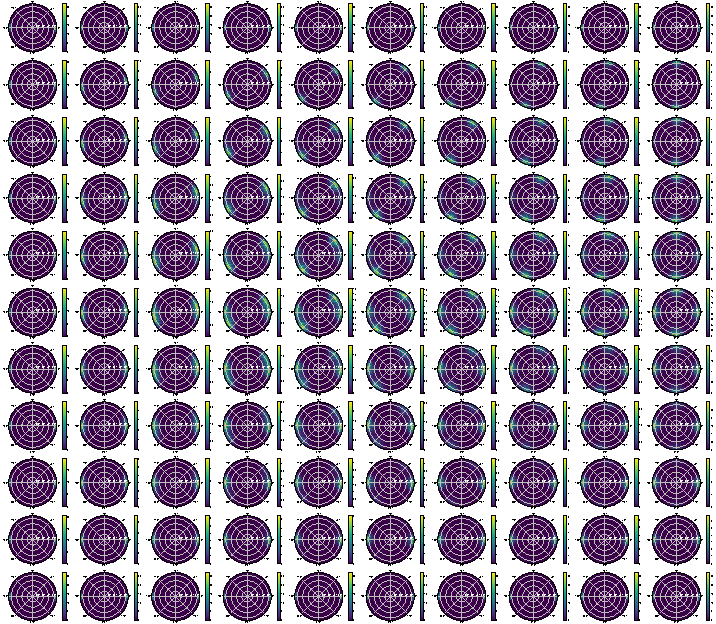
\includegraphics[width=1.0\textwidth]{gfx/model/results/histogram.pdf}};
% \begin{scope}[overlay]
%     \draw[->,thick] ($(image.north west)-(0.25,-0.25)$) -- ++(1,0) node [midway, above] {$\Omega$};
%     \draw[->,thick] ($(image.north west)-(0.25,-0.25)$) -- ++(0,-1) node [midway, above, rotate=90] {$\Psi$};
% \end{scope}
% \path ($(image.north west) + (-.5,.5)$) -- ($(image.north east) + (.5,.5)$);
% \end{tikzpicture}
% }
% \caption{Histogram cube\_2pop\_model}
% \label{app:model_histogram}
% \end{figure}
% %
% %
% \begin{figure}[!tb]
% \centering
% \resizebox{1.0\textwidth}{!}{
% \begin{tikzpicture}[>=latex]
% \node[inner sep=0pt] (image) at (0,0)
%     {\includegraphics[width=1.0\textwidth]{gfx/model/results/voxel_size_simulation_analysis.pdf}};
% \begin{scope}[overlay]
%     \draw[->,thick] ($(image.north west)-(0.25,-0.25)$) -- ++(1,0) node [midway, above] {$voxel_size$};
%     \draw[->,thick] ($(image.north west)-(0.25,-0.25)$) -- ++(0,-1) node [midway, above, rotate=90] {$f0_inc$};
% \end{scope}
% \path ($(image.north west) + (-.5,.5)$) -- ($(image.north east) + (.5,.5)$);
% \end{tikzpicture}
% }
% \vspace{-1ex}
% \begin{center}
% \begin{tikzpicture}
%     \draw[thin] (-3.0,-0.625) rectangle (3.0,0.25);
%     \draw [green!50!black] (-2.5,0) -- (-1.5,0) node [below, midway, black] {truth};
%     \draw [red,dashed] (-0.5,0) -- (0.5,0) node [below, midway, black] {model=r};
%     \draw [blue, dash dot] (1.5,0) -- (2.5,0) node [below, midway, black] {model=p};
% \end{tikzpicture}
% \end{center}
% \caption{voxel\_size\_5\_}
% \label{app:model_histogram}
% \end{figure}
% %
% \begin{figure}[!tb]
% \centering
% \resizebox{1.0\textwidth}{!}{
% \begin{tikzpicture}[>=latex]
% \node[inner sep=0pt] (image) at (0,0)
%     {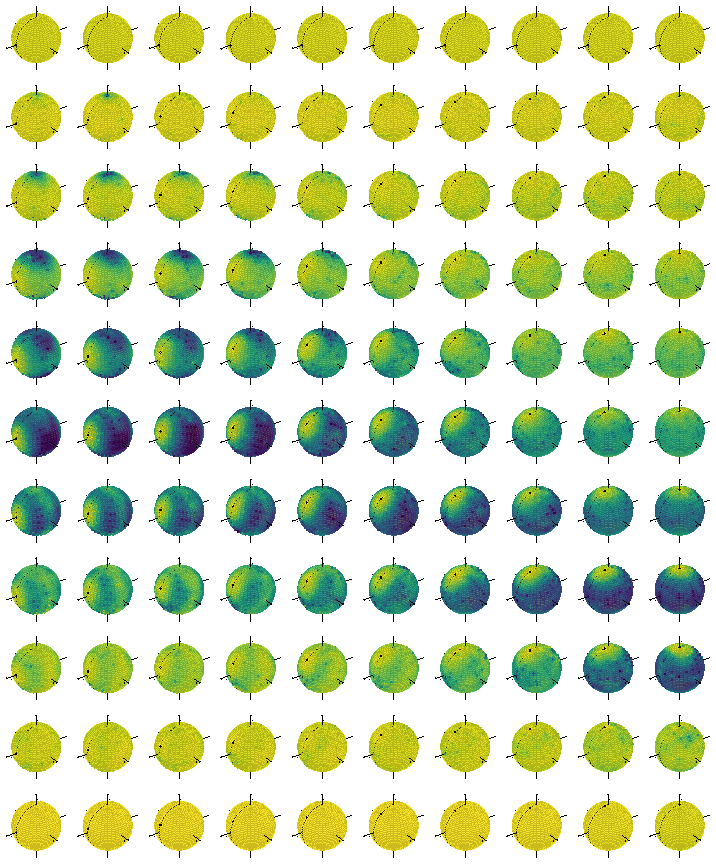
\includegraphics[width=1.0\textwidth]{gfx/simpli/results/simulation_analysis_spheres_LAP_p.pdf}};
% \begin{scope}[overlay]
%     \draw[->,thick] ($(image.north west)-(0.25,-0.25)$) -- ++(1,0) node [midway, above] {$\mathfrak{f}_0^\alpha$};
%     \draw[->,thick] ($(image.north west)-(0.25,-0.25)$) -- ++(0,-1) node [midway, above, rotate=90] {$\mathfrak{f}_0^\Psi$};
% \end{scope}
% \path ($(image.north west) + (-.5,.5)$) -- ($(image.north east) + (.5,.5)$);
% \end{tikzpicture}
% }
% \caption{Sphere LAP p}
% \label{app:model_histogram}
% \end{figure}
% %
% \begin{figure}[!tb]
% \centering
% \resizebox{1.0\textwidth}{!}{
% \begin{tikzpicture}[>=latex]
% \node[inner sep=0pt] (image) at (0,0)
%     {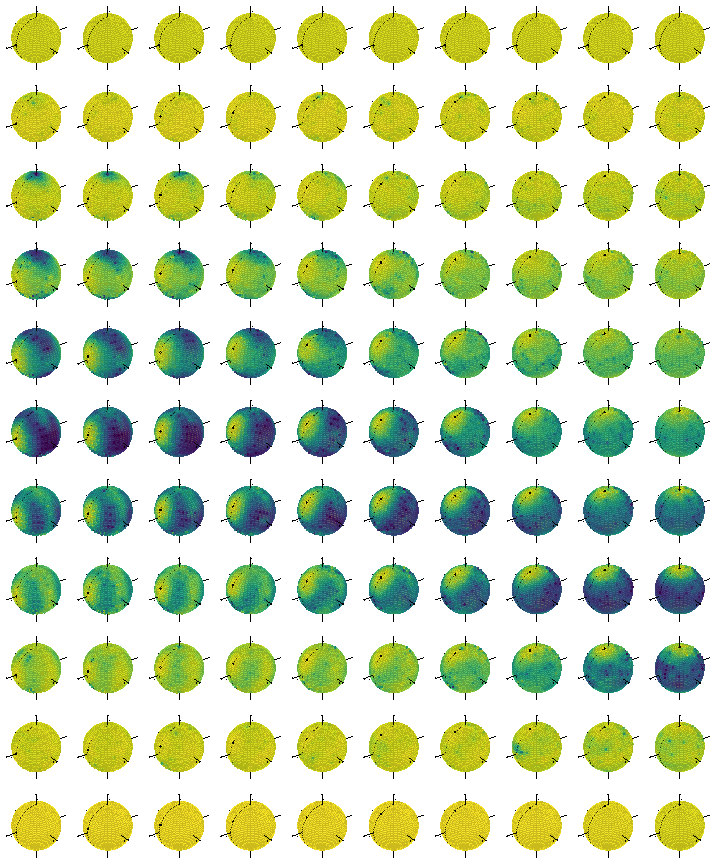
\includegraphics[width=1.0\textwidth]{gfx/simpli/results/simulation_analysis_spheres_LAP_r.pdf}};
% \begin{scope}[overlay]
%     \draw[->,thick] (image.north west) -- ++(1,0) node [midway, above] {$\alpha_0$};
%     \draw[->,thick] (image.north west) -- ++(0,-1) node [midway, above, rotate=90] {$\Psi_0$};
% \end{scope}
% \path ($(image.north west) + (-.5,.5)$) -- ($(image.north east) + (.5,.5)$);
% \end{tikzpicture}
% }
% \caption{Sphere LAP r}
% \label{app:model_histogram}
% \end{figure}
% %
% \begin{figure}[!tb]
% \centering
% \resizebox{1.0\textwidth}{!}{
% \begin{tikzpicture}[>=latex]
% \node[inner sep=0pt] (image) at (0,0)
%     {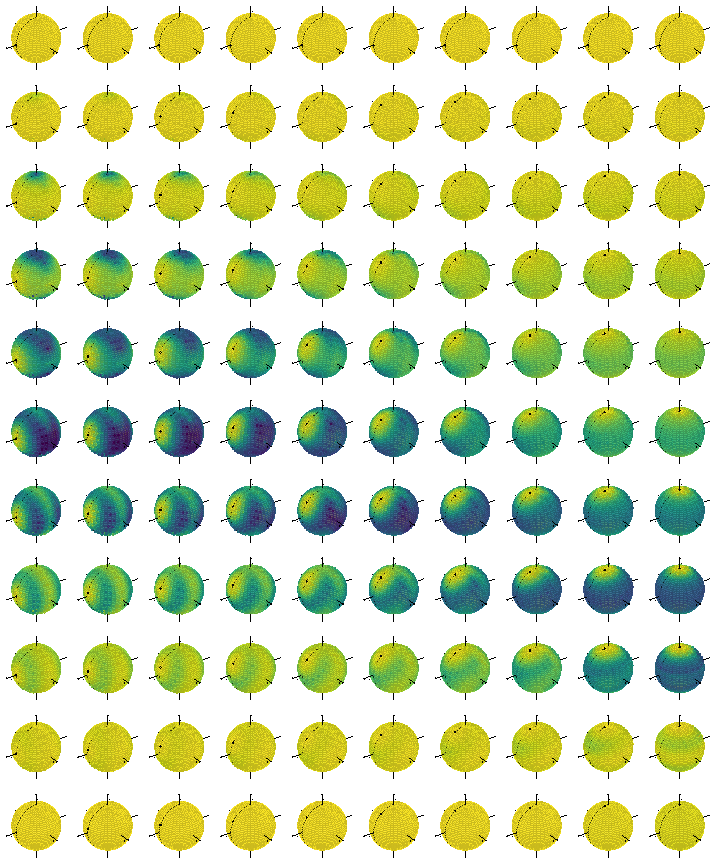
\includegraphics[width=1.0\textwidth]{gfx/simpli/results/simulation_analysis_spheres_PM_p.pdf}};
% \begin{scope}[overlay]
%     \draw[->,thick] ($(image.north west)-(0.25,-0.25)$) -- ++(1,0) node [midway, above] {$f_0$};
%     \draw[->,thick] ($(image.north west)-(0.25,-0.25)$) -- ++(0,-1) node [midway, above, rotate=90] {$\Psi$};
% \end{scope}
% \path ($(image.north west) + (-.5,.5)$) -- ($(image.north east) + (.5,.5)$);
% \end{tikzpicture}
% }
% \caption{Sphere PM p}
% \label{app:model_histogram}
% \end{figure}
% %
% \begin{figure}[!tb]
% \centering
% \resizebox{1.0\textwidth}{!}{
% \begin{tikzpicture}[>=latex]
% \node[inner sep=0pt] (image) at (0,0)
%     {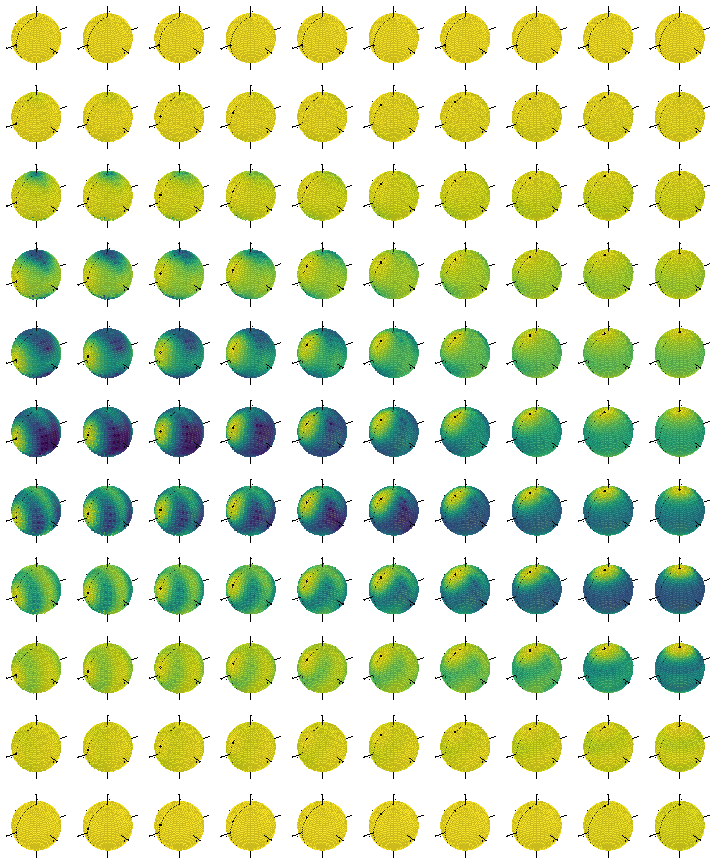
\includegraphics[width=1.0\textwidth]{gfx/simpli/results/simulation_analysis_spheres_PM_r.pdf}};
% \begin{scope}[overlay]
%     \draw[->,thick] ($(image.north west)-(0.25,-0.25)$) -- ++(1,0) node [midway, above] {$f_0$};
%     \draw[->,thick] ($(image.north west)-(0.25,-0.25)$) -- ++(0,-1) node [midway, above, rotate=90] {$\Psi$};
% \end{scope}
% \path ($(image.north west) + (-.5,.5)$) -- ($(image.north east) + (.5,.5)$);
% \end{tikzpicture}
% }
% \caption{Sphere PM r}
% \label{app:model_histogram}
% \end{figure}
% %
% \begin{figure}[!t]
% \centering
% \resizebox{1.0\textwidth}{!}{
% \includegraphics[width=\textwidth, page=2]{dev/rc1/cube_2pop_orientation_hist2d_output_cube_2pop_135_rc1.pdf}
% }
% \caption[Model orientation histograms]{density distribution of fiber segment orientation in initial and resulting models for $\fiberRadius = \SI{1}{\micro\meter}$. \itodo{fit ESAG} \ITODO{these are only resulting models!}}
% \label{app:modelOrientation}
% \end{figure}
% %
% %
%
\chapter{} % Model analysis
\label{app:modelAnalysis}
%
%
\fakesection{Model parameter}
%
\begin{figure}[!h]
    \centering
    \includegraphics[width=1\textwidth]{dev/rc1/mpara/pre_stats_box_plot_volume_output_parameter_statistic_rc1.pdf}
    \caption{Caption}
    \label{app:appModelVolumeBoxPlot}
\end{figure}
%
% % \foreach \n in {1,3,...,10}{
% % \begin{landscape}
% \begin{figure}[!t]
% \centering
% % \resizebox{\textwidth}{!}{
% \includegraphics[width=\textwidth,page=1]{dev/rc1/mpara/pre_stats_time_evolve_all_output_parameter_statistic_rc1.pdf}
% \includegraphics[width=\textwidth,page=2]{dev/rc1/mpara/pre_stats_time_evolve_all_output_parameter_statistic_rc1.pdf}
% \end{figure}
% % \end{landscape}
%
%
\fakesection{Time evolution}
%
\setlength{\tikzwidth}{\textwidth}
\begin{sidewaysfigure}[]
\centering
\includegraphics[height=\tikzwidth,page=1]{dev/rc1/mpara/pre_stats_time_evolve_all_output_parameter_statistic_rc1.pdf}
\includegraphics[height=\tikzwidth,page=2]{dev/rc1/mpara/pre_stats_time_evolve_all_output_parameter_statistic_rc1.pdf}
\label{app:pste1}
\end{sidewaysfigure}
%
\begin{sidewaysfigure}[]
\centering
% \resizebox{\tikzwidth}{!}{
\includegraphics[height=\tikzwidth,page=3]{dev/rc1/mpara/pre_stats_time_evolve_all_output_parameter_statistic_rc1.pdf}
\includegraphics[height=\tikzwidth,page=4]{dev/rc1/mpara/pre_stats_time_evolve_all_output_parameter_statistic_rc1.pdf}
% }
\label{app:pste2}
\end{sidewaysfigure}
%
\begin{sidewaysfigure}[]
\centering
% \resizebox{\textwidth}{!}{
\includegraphics[height=\tikzwidth,page=5]{dev/rc1/mpara/pre_stats_time_evolve_all_output_parameter_statistic_rc1.pdf}
\includegraphics[height=\tikzwidth,page=6]{dev/rc1/mpara/pre_stats_time_evolve_all_output_parameter_statistic_rc1.pdf}
\label{app:pste3}
\end{sidewaysfigure}
%
\begin{sidewaysfigure}[]
\centering
% \resizebox{\textwidth}{!}{
\includegraphics[height=\tikzwidth,page=7]{dev/rc1/mpara/pre_stats_time_evolve_all_output_parameter_statistic_rc1.pdf}
\includegraphics[height=\tikzwidth,page=8]{dev/rc1/mpara/pre_stats_time_evolve_all_output_parameter_statistic_rc1.pdf}
\label{app:pste4}
\end{sidewaysfigure}
%
\begin{sidewaysfigure}[]
\centering
% \resizebox{\textwidth}{!}{
\includegraphics[height=\tikzwidth,page=9]{dev/rc1/mpara/pre_stats_time_evolve_all_output_parameter_statistic_rc1.pdf}
\includegraphics[height=\tikzwidth,page=10]{dev/rc1/mpara/pre_stats_time_evolve_all_output_parameter_statistic_rc1.pdf}
\label{app:pste5}
\end{sidewaysfigure}
%
%
\fakesection{Histogramms}
%
\begin{figure}
    \centering
    \includegraphics[width=\textwidth, page=2]{dev/rc1/cube_2pop_orientation_hist2d_output_cube_2pop_135_rc1.pdf}
    \caption{Caption}
    \label{app:modelHistOrientation}
\end{figure}[]
%
\fakesection{Speedup}
%
\begin{figure}[!t]
\centering
\includegraphics[page=2]{dev/rc1/speed/boxplot_output_r_0.5.pkl_speedup.csv.pdf}
\caption[\code{model.Sovler} speedup]{\code{model.Sovler} speedup. The time measurements are taken after $\Delta_{\mathit{steps}}$ for the next $\SI{25}{\steps}$ for parallel $(||)$ and crossing $(\times)$ fiber configurations.}
\label{app:solverSpeedupAll}
\end{figure}
%
%
%
\fakesection{Simulation Library}
\begin{table}[htb]
\centering
\caption[Opening angle distribution]{Orientation statistic of simulation model library.}
\resizebox{\textwidth}{!}{
\pgfplotstabletypeset[%
    thesisTableStyle,
    columns={omega,psi,pop,incl_mean,incl_std,incl_25,incl_50,incl_75,phi_mean,phi_std,phi_25,phi_50,phi_75,mean,std,25,50,75},
    every head row/.style={
        before row={
            \toprule
        },
        after row={$\si{\degree}$ & & & $\si{\degree}$ & $\si{\degree}$ & $\si{\degree}$ & $\si{\degree}$ & $\si{\degree}$ & $\si{\degree}$ & $\si{\degree}$ & $\si{\degree}$ & $\si{\degree}$ & $\si{\degree}$ & $\si{\degree}$ & $\si{\degree}$ & $\si{\degree}$ & $\si{\degree}$ & $\si{\degree}$ \\ \midrule},
    },
    columns/omega/.style={column name=$\Omega$},
    columns/psi/.style={column name=$\Psi$},
    columns/mean/.style={column name=$<d\Omega>$,zerofill,precision=0},
    columns/std/.style={column name=$\sigma(d\Omega)$,zerofill,precision=0},
    columns/25/.style={column name=$25(d\Omega)$,zerofill,precision=0},
    columns/50/.style={column name=$50(d\Omega)$,zerofill,precision=0},
    columns/75/.style={column name=$75(d\Omega)$,zerofill,precision=0},
    columns/incl_mean/.style={column name=$<\alpha>$,fixed,fixed zerofill,precision=0},
    columns/incl_std/.style={column name=$\sigma(\alpha)$,fixed,fixed zerofill,precision=0},
    columns/incl_25/.style={column name=$25(\alpha)$,fixed,fixed zerofill,precision=0},
    columns/incl_50/.style={column name=$50(\alpha)$,fixed,fixed zerofill,precision=0},
    columns/incl_75/.style={column name=$75(\alpha)$,fixed,fixed zerofill,precision=0},
    columns/phi_mean/.style={column name=$<\varphi>$,fixed,fixed zerofill,precision=0},
    columns/phi_std/.style={column name=$\sigma(\varphi)$,fixed,fixed zerofill,precision=0},
    columns/phi_25/.style={column name=$25(\varphi)$,fixed,fixed zerofill,precision=0},
    columns/phi_50/.style={column name=$50(\varphi)$,fixed,fixed zerofill,precision=0},
    columns/phi_75/.style={column name=$75(\varphi)$,fixed,fixed zerofill,precision=0},
    col sep=comma,
    %
]
{dev/rc1/domega/omegas_ms_2pop.csv}
}
\label{app:modelDistribution}
\end{table}
%
% 
%
\chapter{}
\label{app:Simulation}
%
\fakesection{Tissue}
%
\begin{sidewaysfigure}[!p]
\resizebox{\textheight}{!}{
\begin{tabular}{cc}
\includegraphics[]{dev/rc1/tissue/bf_rc1_retardation_PM_Roden.pdf}&
\includegraphics[]{dev/rc1/tissue/bf_rc1_retardation_PM_Human.pdf}\\
\includegraphics[]{dev/rc1/tissue/bf_rc1_transmittance_PM_Roden.pdf}&
\includegraphics[]{dev/rc1/tissue/bf_rc1_transmittance_PM_Human.pdf}
\end{tabular}}
\end{sidewaysfigure}
%
\fakesection{Voxelsize}
%
\begin{figure}[!p]
% 2_simulation/0_parameter/fiber_radii.py
\centering
\includegraphics[width=\textwidth, page=1]{dev/rc1/voxel_size/voxel_size_plots_data_output_vs_135_0.01_6_25_vervet_r_rc1.pdf}
\caption[voxel size model with noise]{The mean difference is constant for smaller voxel sizes and does not start to grow significantly before $\voxels=\SI{0.125}{\micro\meter}$.}
\label{app:voxelsizeNoise}
\end{figure}
%
%
%
\fakesection{domega}
%
\begin{figure}[!t]
    \centering
    \includegraphics[]{dev/rc1/domega/cube_2pop_domega_analysis_all_output.pdf}
    \caption{Direction and inclination distribution of simulation model library.}
    % \label{fig:my_label}
\end{figure}
%
%
%
% %%%%%%%%%%%%%%%%%%%%%%%%%%%%%%%%%%%%%%%%%%%%%%%%%%%%%%%%%%%
% SINGLE
% %%%%%%%%%%%%%%%%%%%%%%%%%%%%%%%%%%%%%%%%%%%%%%%%%%%%%%%%%%%
%
\fakesection{Single fiber population}
%
\begin{figure}[!p]
\centering
% \begin{minipage}{0.45\textwidth}
\resizebox{\textwidth}{!}{
\rotatebox{90}{
\begin{tabular}{c|c}
\begin{tabular}{c|c}
    \includegraphics[]{dev/rc1/single/cube_2pop_135_rc1_single_plots_single_pop_hist_0.0.pdf} &
    \includegraphics[]{dev/rc1/single/cube_2pop_135_rc1_single_plots_single_pop_hist_25.0.pdf} \\
    \includegraphics[]{dev/rc1/single/cube_2pop_135_rc1_single_plots_single_pop_hist_5.0.pdf} &
    \includegraphics[]{dev/rc1/single/cube_2pop_135_rc1_single_plots_single_pop_hist_30.0.pdf} \\
    \includegraphics[]{dev/rc1/single/cube_2pop_135_rc1_single_plots_single_pop_hist_10.0.pdf} &
    \includegraphics[]{dev/rc1/single/cube_2pop_135_rc1_single_plots_single_pop_hist_35.0.pdf} \\
    \includegraphics[]{dev/rc1/single/cube_2pop_135_rc1_single_plots_single_pop_hist_15.0.pdf} &
    \includegraphics[]{dev/rc1/single/cube_2pop_135_rc1_single_plots_single_pop_hist_40.0.pdf} \\
    \includegraphics[]{dev/rc1/single/cube_2pop_135_rc1_single_plots_single_pop_hist_20.0.pdf} &
    \includegraphics[]{dev/rc1/single/cube_2pop_135_rc1_single_plots_single_pop_hist_45.0.pdf}
\end{tabular}
&
\begin{tabular}{c|c}
    \includegraphics[]{dev/rc1/single/cube_2pop_135_rc1_single_plots_single_pop_hist_50.0.pdf} &
    \includegraphics[]{dev/rc1/single/cube_2pop_135_rc1_single_plots_single_pop_hist_75.0.pdf} \\
    \includegraphics[]{dev/rc1/single/cube_2pop_135_rc1_single_plots_single_pop_hist_55.0.pdf} &
    \includegraphics[]{dev/rc1/single/cube_2pop_135_rc1_single_plots_single_pop_hist_80.0.pdf} \\
    \includegraphics[]{dev/rc1/single/cube_2pop_135_rc1_single_plots_single_pop_hist_60.0.pdf} &
    \includegraphics[]{dev/rc1/single/cube_2pop_135_rc1_single_plots_single_pop_hist_85.0.pdf} \\
    \includegraphics[]{dev/rc1/single/cube_2pop_135_rc1_single_plots_single_pop_hist_65.0.pdf} &
    \includegraphics[]{dev/rc1/single/cube_2pop_135_rc1_single_plots_single_pop_hist_90.0.pdf} \\
    \includegraphics[]{dev/rc1/single/cube_2pop_135_rc1_single_plots_single_pop_hist_70.0.pdf} &
\end{tabular}
\end{tabular}
}}
%
\caption[sim]{left: 2d log histogramm orientation from rofl analysis of simulation, right: 2d log histogramm of orientation of model segemnts. \itodo{rfc plots}}
\label{app:single_fiber_pop_hist_app}
\end{figure}
%
%
% %%%%%%%%%%%%%%%%%%%%%%%%%%%%%%%%%%%%%%%%%%%%%%%%%%%%%%%%%%%
% FLAT
% %%%%%%%%%%%%%%%%%%%%%%%%%%%%%%%%%%%%%%%%%%%%%%%%%%%%%%%%%%%
%
\fakesection{Crossing fiber population}
%
\begin{figure}[!p]
\centering
\setlength{\tikzwidth}{0.45\textwidth}
\begin{tabular}{c|c}
    \includegraphics[width=\tikzwidth]{dev/rc1/flat/cube_2pop_135_rc1_flat_plots_flat_pop_hist_omega_0.0_psi_0.3.pdf} &
    \includegraphics[width=\tikzwidth]{dev/rc1/flat/cube_2pop_135_rc1_flat_plots_flat_pop_hist_omega_50.0_psi_0.3.pdf} \\
    \includegraphics[width=\tikzwidth]{dev/rc1/flat/cube_2pop_135_rc1_flat_plots_flat_pop_hist_omega_10.0_psi_0.3.pdf} &
    \includegraphics[width=\tikzwidth]{dev/rc1/flat/cube_2pop_135_rc1_flat_plots_flat_pop_hist_omega_60.0_psi_0.3.pdf} \\
    \includegraphics[width=\tikzwidth]{dev/rc1/flat/cube_2pop_135_rc1_flat_plots_flat_pop_hist_omega_20.0_psi_0.3.pdf} &
    \includegraphics[width=\tikzwidth]{dev/rc1/flat/cube_2pop_135_rc1_flat_plots_flat_pop_hist_omega_70.0_psi_0.3.pdf} \\
    \includegraphics[width=\tikzwidth]{dev/rc1/flat/cube_2pop_135_rc1_flat_plots_flat_pop_hist_omega_30.0_psi_0.3.pdf} &
    \includegraphics[width=\tikzwidth]{dev/rc1/flat/cube_2pop_135_rc1_flat_plots_flat_pop_hist_omega_80.0_psi_0.3.pdf} \\
    \includegraphics[width=\tikzwidth]{dev/rc1/flat/cube_2pop_135_rc1_flat_plots_flat_pop_hist_omega_40.0_psi_0.3.pdf} &
    \includegraphics[width=\tikzwidth]{dev/rc1/flat/cube_2pop_135_rc1_flat_plots_flat_pop_hist_omega_90.0_psi_0.3.pdf}
\end{tabular}
%
\caption[sim]{psi=0.3; left: 2d log histogramm orientation from rofl analysis of simulation, right: 2d log histogram of orientation of model segemnts. \itodo{legende}}
\label{app:flat_03_fiber_pop_hist}
\end{figure}
%
%
%
%
\begin{figure}[!p]
\centering
\setlength{\tikzwidth}{0.45\textwidth}
\begin{tabular}{c|c}
    \includegraphics[width=\tikzwidth]{dev/rc1/flat/cube_2pop_135_rc1_flat_plots_flat_pop_hist_omega_0.0_psi_0.5.pdf} &
    \includegraphics[width=\tikzwidth]{dev/rc1/flat/cube_2pop_135_rc1_flat_plots_flat_pop_hist_omega_50.0_psi_0.5.pdf} \\
    \includegraphics[width=\tikzwidth]{dev/rc1/flat/cube_2pop_135_rc1_flat_plots_flat_pop_hist_omega_10.0_psi_0.5.pdf} &
    \includegraphics[width=\tikzwidth]{dev/rc1/flat/cube_2pop_135_rc1_flat_plots_flat_pop_hist_omega_60.0_psi_0.5.pdf} \\
    \includegraphics[width=\tikzwidth]{dev/rc1/flat/cube_2pop_135_rc1_flat_plots_flat_pop_hist_omega_20.0_psi_0.5.pdf} &
    \includegraphics[width=\tikzwidth]{dev/rc1/flat/cube_2pop_135_rc1_flat_plots_flat_pop_hist_omega_70.0_psi_0.5.pdf} \\
    \includegraphics[width=\tikzwidth]{dev/rc1/flat/cube_2pop_135_rc1_flat_plots_flat_pop_hist_omega_30.0_psi_0.5.pdf} &
    \includegraphics[width=\tikzwidth]{dev/rc1/flat/cube_2pop_135_rc1_flat_plots_flat_pop_hist_omega_80.0_psi_0.5.pdf} \\
    \includegraphics[width=\tikzwidth]{dev/rc1/flat/cube_2pop_135_rc1_flat_plots_flat_pop_hist_omega_40.0_psi_0.5.pdf} &
    \includegraphics[width=\tikzwidth]{dev/rc1/flat/cube_2pop_135_rc1_flat_plots_flat_pop_hist_omega_90.0_psi_0.5.pdf}
\end{tabular}
%
\caption[sim]{psi=0.5; left: 2d log histogramm orientation from rofl analysis of simulation, right: 2d log histogramm of orientation of model segemnts. \itodo{legende}}
\label{app:flat_05_fiber_pop_hist}
\end{figure}
%
%
%
\begin{figure}[!p]
\centering
\resizebox{\textwidth}{!}{
\begin{tabular}{cc}
\includegraphics[page=1]{dev/rc1/analysis/plots_flat_pop_output_cube_2pop_135_rc1_flat.pdf} &
\includegraphics[page=2]{dev/rc1/analysis/plots_flat_pop_output_cube_2pop_135_rc1_flat.pdf}\\
\includegraphics[page=3]{dev/rc1/analysis/plots_flat_pop_output_cube_2pop_135_rc1_flat.pdf} &
\includegraphics[page=4]{dev/rc1/analysis/plots_flat_pop_output_cube_2pop_135_rc1_flat.pdf}
\end{tabular}
}
\end{figure}
%
\begin{figure}[!p]
\centering
\resizebox{\textwidth}{!}{
\begin{tabular}{cc}
\includegraphics[page=5]{dev/rc1/analysis/plots_flat_pop_output_cube_2pop_135_rc1_flat.pdf} &
\includegraphics[page=6]{dev/rc1/analysis/plots_flat_pop_output_cube_2pop_135_rc1_flat.pdf}\\
\includegraphics[page=7]{dev/rc1/analysis/plots_flat_pop_output_cube_2pop_135_rc1_flat.pdf} &
\includegraphics[page=8]{dev/rc1/analysis/plots_flat_pop_output_cube_2pop_135_rc1_flat.pdf}
\end{tabular}
}
\end{figure}
%
\begin{figure}[]
\centering
\resizebox{\textwidth}{!}{
\begin{tabular}{cc}
\includegraphics[page=9]{dev/rc1/analysis/plots_flat_pop_output_cube_2pop_135_rc1_flat.pdf} &
\includegraphics[page=10]{dev/rc1/analysis/plots_flat_pop_output_cube_2pop_135_rc1_flat.pdf}
\end{tabular}
}
\end{figure}
%
%
% %%%%%%%%%%%%%%%%%%%%%%%%%%%%%%%%%%%%%%%%%%%%%%%%%%%%%%%%%%%
% INCLINED
% %%%%%%%%%%%%%%%%%%%%%%%%%%%%%%%%%%%%%%%%%%%%%%%%%%%%%%%%%%%
%
\fakesection{Inclined fiber population}
%
\begin{figure}[!p]
\centering
\setlength{\tikzwidth}{0.45\textwidth}
\begin{tabular}{c|c}
    \includegraphics[width=\tikzwidth]{dev/rc1/inclined/cube_2pop_135_rc1_inclined_plots_inclined_pop_hist_omega_0.0_psi_0.3.pdf} &
    \includegraphics[width=\tikzwidth]{dev/rc1/inclined/cube_2pop_135_rc1_inclined_plots_inclined_pop_hist_omega_50.0_psi_0.3.pdf} \\ \includegraphics[width=\tikzwidth]{dev/rc1/inclined/cube_2pop_135_rc1_inclined_plots_inclined_pop_hist_omega_10.0_psi_0.3.pdf} & \includegraphics[width=\tikzwidth]{dev/rc1/inclined/cube_2pop_135_rc1_inclined_plots_inclined_pop_hist_omega_60.0_psi_0.3.pdf} \\
    \includegraphics[width=\tikzwidth]{dev/rc1/inclined/cube_2pop_135_rc1_inclined_plots_inclined_pop_hist_omega_20.0_psi_0.3.pdf} &
    \includegraphics[width=\tikzwidth]{dev/rc1/inclined/cube_2pop_135_rc1_inclined_plots_inclined_pop_hist_omega_70.0_psi_0.3.pdf} \\ \includegraphics[width=\tikzwidth]{dev/rc1/inclined/cube_2pop_135_rc1_inclined_plots_inclined_pop_hist_omega_30.0_psi_0.3.pdf} & \includegraphics[width=\tikzwidth]{dev/rc1/inclined/cube_2pop_135_rc1_inclined_plots_inclined_pop_hist_omega_80.0_psi_0.3.pdf} \\
    \includegraphics[width=\tikzwidth]{dev/rc1/inclined/cube_2pop_135_rc1_inclined_plots_inclined_pop_hist_omega_40.0_psi_0.3.pdf} &
    \includegraphics[width=\tikzwidth]{dev/rc1/inclined/cube_2pop_135_rc1_inclined_plots_inclined_pop_hist_omega_90.0_psi_0.3.pdf}
\end{tabular}
%
\caption[sim]{psi=0.3; left: 2d log histogramm orientation from rofl analysis of simulation, right: 2d log histogram of orientation of model segemnts. \itodo{legende}}
\label{app:incl_03_fiber_pop_hist}
\end{figure}
%
%
%
%
\begin{figure}[!p]
\centering
\setlength{\tikzwidth}{0.45\textwidth}
\begin{tabular}{c|c}
    \includegraphics[width=\tikzwidth]{dev/rc1/inclined/cube_2pop_135_rc1_inclined_plots_inclined_pop_hist_omega_0.0_psi_0.5.pdf} &
    \includegraphics[width=\tikzwidth]{dev/rc1/inclined/cube_2pop_135_rc1_inclined_plots_inclined_pop_hist_omega_50.0_psi_0.5.pdf} \\
    \includegraphics[width=\tikzwidth]{dev/rc1/inclined/cube_2pop_135_rc1_inclined_plots_inclined_pop_hist_omega_10.0_psi_0.5.pdf} &
    \includegraphics[width=\tikzwidth]{dev/rc1/inclined/cube_2pop_135_rc1_inclined_plots_inclined_pop_hist_omega_60.0_psi_0.5.pdf} \\
    \includegraphics[width=\tikzwidth]{dev/rc1/inclined/cube_2pop_135_rc1_inclined_plots_inclined_pop_hist_omega_20.0_psi_0.5.pdf} &
    \includegraphics[width=\tikzwidth]{dev/rc1/inclined/cube_2pop_135_rc1_inclined_plots_inclined_pop_hist_omega_70.0_psi_0.5.pdf} \\
    \includegraphics[width=\tikzwidth]{dev/rc1/inclined/cube_2pop_135_rc1_inclined_plots_inclined_pop_hist_omega_30.0_psi_0.5.pdf} &
    \includegraphics[width=\tikzwidth]{dev/rc1/inclined/cube_2pop_135_rc1_inclined_plots_inclined_pop_hist_omega_80.0_psi_0.5.pdf} \\
    \includegraphics[width=\tikzwidth]{dev/rc1/inclined/cube_2pop_135_rc1_inclined_plots_inclined_pop_hist_omega_40.0_psi_0.5.pdf} &
    \includegraphics[width=\tikzwidth]{dev/rc1/inclined/cube_2pop_135_rc1_inclined_plots_inclined_pop_hist_omega_90.0_psi_0.5.pdf}
\end{tabular}
%
\caption[sim]{psi=0.5; left: 2d log histogramm orientation from rofl analysis of simulation, right: 2d log histogramm of orientation of model segemnts. \itodo{legende}}
\label{app:incl_05_fiber_pop_hist}
\end{figure}
%
%
%
\begin{figure}[!p]
\centering
\resizebox{\textwidth}{!}{
\begin{tabular}{cc}
\includegraphics[page=1]{dev/rc1/analysis/plots_inclined_pop_output_cube_2pop_135_rc1_inclined.pdf} &
\includegraphics[page=2]{dev/rc1/analysis/plots_inclined_pop_output_cube_2pop_135_rc1_inclined.pdf}\\
\includegraphics[page=3]{dev/rc1/analysis/plots_inclined_pop_output_cube_2pop_135_rc1_inclined.pdf} &
\includegraphics[page=4]{dev/rc1/analysis/plots_inclined_pop_output_cube_2pop_135_rc1_inclined.pdf}
\end{tabular}
}
\end{figure}
%
\begin{figure}[!p]
\centering
\resizebox{\textwidth}{!}{
\begin{tabular}{cc}
\includegraphics[page=5]{dev/rc1/analysis/plots_inclined_pop_output_cube_2pop_135_rc1_inclined.pdf} &
\includegraphics[page=6]{dev/rc1/analysis/plots_inclined_pop_output_cube_2pop_135_rc1_inclined.pdf}\\
\includegraphics[page=7]{dev/rc1/analysis/plots_inclined_pop_output_cube_2pop_135_rc1_inclined.pdf} &
\includegraphics[page=8]{dev/rc1/analysis/plots_inclined_pop_output_cube_2pop_135_rc1_inclined.pdf}
\end{tabular}
}
\end{figure}
%
\begin{figure}[!p]
\centering
\resizebox{\textwidth}{!}{
\begin{tabular}{cc}
\includegraphics[page=9]{dev/rc1/analysis/plots_inclined_pop_output_cube_2pop_135_rc1_inclined.pdf} &
\includegraphics[page=10]{dev/rc1/analysis/plots_inclined_pop_output_cube_2pop_135_rc1_inclined.pdf}
\end{tabular}
}
\end{figure}
%
% %
% %
%
% \newpage
% \mbox{}
%
% **************************************************
% End of Document CONTENT
% **************************************************
\end{document}
